% Chapter 5b: Multivariate GARCH Models
% Harvard-quality academic presentation
% Bachelor program, Bucharest University of Economic Studies

\documentclass[9pt, aspectratio=169, t]{beamer}
\input{preamble}
\subtitle{Chapter 5b: Multivariate GARCH Models}

\begin{document}

% Title page (no header/footer)
{
\setbeamertemplate{headline}{}
\setbeamertemplate{footline}{}
\begin{frame}
    \titlepage
\end{frame}
}

%=============================================================================
% LEARNING OBJECTIVES
%=============================================================================
\section{Motivation}

\begin{frame}{Learning Objectives}
    \begin{cminipage}{0.95\textwidth}
    {\footnotesize
    \begin{block}{By the end of this chapter, you will be able to:}
        \begin{enumerate}\setlength{\itemsep}{2pt}
            \item Explain why \textbf{multivariate volatility modeling} is necessary
            \item Formulate and estimate \textbf{VEC}, \textbf{BEKK}, \textbf{CCC}, and \textbf{DCC} models
            \item Interpret \textbf{dynamic correlations} and covariance decompositions
            \item Apply multivariate GARCH for \textbf{portfolio optimization}, \textbf{hedging}, and \textbf{risk management}
        \end{enumerate}
    \end{block}
    \vspace{0.1cm}
    \begin{alertblock}{Practical Skills}
        \begin{itemize}\setlength{\itemsep}{0pt}
            \item Python implementation with \texttt{rmgarch} / \texttt{mgarch} packages
            \item Interpreting time-varying covariance matrices
            \item Dynamic hedge ratios and portfolio weights
        \end{itemize}
    \end{alertblock}
    \vspace{0.2cm}
    \textit{\textbf{Key takeaway:} You are not learning models --- you are learning how to measure real portfolio risk.}
    }
    \end{cminipage}
\end{frame}

%=============================================================================
% TABLE OF CONTENTS
%=============================================================================
\begin{frame}{Outline}
    \vspace{-0.3cm}
    {\small
    \begin{columns}[T]
        \begin{column}{0.48\textwidth}
            \begin{block}{Foundations}
                \begin{itemize}\setlength{\itemsep}{3pt}
                    \item Motivation: From Univariate to Multivariate
                    \item The Multivariate GARCH Framework
                    \item VEC and Diagonal VEC Models
                    \item The BEKK Model
                    \item Constant Conditional Correlation (CCC)
                    \item Dynamic Conditional Correlation (DCC)
                \end{itemize}
            \end{block}
        \end{column}
        \begin{column}{0.48\textwidth}
            \begin{exampleblock}{Applications}
                \begin{itemize}\setlength{\itemsep}{3pt}
                    \item Other Multivariate GARCH Models
                    \item Estimation and the Curse of Dimensionality
                    \item Model Selection and Diagnostics
                    \item Portfolio Optimization
                    \item Dynamic Hedging
                    \item Summary and Quiz
                \end{itemize}
            \end{exampleblock}
        \end{column}
    \end{columns}
    }
\end{frame}

%=============================================================================
% STORY OF THE CHAPTER
%=============================================================================

\begin{frame}{The Story of This Chapter}
    \begin{cminipage}{0.95\textwidth}
    {\footnotesize
    \begin{block}{The Problem}
        \begin{itemize}\setlength{\itemsep}{0pt}
            \item Correlations between assets \textbf{change over time} --- and they spike during crises
            \item Ignoring this leads to wrong portfolios, bad hedges, and underestimated risk
        \end{itemize}
    \end{block}
    \begin{block}{The Difficulty}
        \begin{itemize}\setlength{\itemsep}{0pt}
            \item Modeling $N$ assets requires $N(N+1)/2$ time-varying covariance elements
            \item The \textbf{curse of dimensionality} makes most approaches infeasible
        \end{itemize}
    \end{block}
    \begin{alertblock}{The Solutions (from general to practical)}
        \begin{itemize}\setlength{\itemsep}{2pt}
            \item \textbf{VEC}: the most general model --- but unusable in practice
            \item \textbf{BEKK}: guarantees positive definiteness --- but does not scale
            \item \textbf{CCC}: simple and fast --- but correlations are \textit{constant} (wrong!)
            \item \textcolor{Crimson}{\textbf{DCC}}: the optimal compromise --- dynamic correlations with \textbf{only 2 extra parameters}
        \end{itemize}
    \end{alertblock}
    }
    \end{cminipage}
\end{frame}

%=============================================================================
% SECTION 1: MOTIVATION
%=============================================================================
\section{From Univariate to Multivariate}

\begin{frame}{Why Go Multivariate?}
    \begin{cminipage}{0.95\textwidth}
    {\footnotesize
    \begin{block}{The Problem}
        \begin{itemize}\setlength{\itemsep}{2pt}
            \item Univariate GARCH models each asset's volatility \textbf{in isolation}
            \item They ignore \textbf{co-movements} between assets:
                \begin{itemize}\setlength{\itemsep}{0pt}
                    \item How does the volatility of asset $A$ spill over to asset $B$?
                    \item How do correlations between assets change over time?
                \end{itemize}
        \end{itemize}
    \end{block}
    \vspace{0.1cm}
    \begin{alertblock}{But in reality\ldots}
        \begin{itemize}\setlength{\itemsep}{0pt}
            \item Markets are interconnected --- shocks propagate across assets
            \item Financial decisions require the \textbf{full covariance matrix} $\mathbf{H}_t$, not just individual variances
        \end{itemize}
    \end{alertblock}
    \vspace{0.2cm}
    \textit{\textbf{Key insight:} Risk is not the sum of individual risks.}
    }
    \end{cminipage}
\end{frame}

\begin{frame}{The Central Question: Modeling $\mathbf{H}_t$}
    \begin{cminipage}{0.95\textwidth}
    {\footnotesize
    \begin{block}{Setup}
        \begin{itemize}\setlength{\itemsep}{0pt}
            \item Given $N$ assets with return vector $\mathbf{r}_t = (r_{1t}, \ldots, r_{Nt})'$, we need to model:
        \end{itemize}
        \[
            \mathbf{H}_t = \text{Var}(\mathbf{r}_t \mid \mathcal{F}_{t-1})
        \]
        \begin{itemize}\setlength{\itemsep}{0pt}
            \item the \textbf{time-varying conditional covariance matrix}
        \end{itemize}
    \end{block}
    \vspace{0.1cm}
    \begin{alertblock}{Why is this hard?}
        \begin{itemize}\setlength{\itemsep}{0pt}
            \item $\mathbf{H}_t$ has $N(N+1)/2$ unique elements --- for $N = 50$: \textbf{1,275 parameters} at each $t$
            \item Must be \textbf{positive definite} at every time step
            \item Must capture \textbf{dynamic} correlations, not just volatilities
        \end{itemize}
    \end{alertblock}
    \vspace{0.2cm}
    \textit{\textbf{Intuition:} $\mathbf{H}_t$ is the ``weather forecast'' for risk --- it updates daily as new information arrives.}
    }
    \end{cminipage}
\end{frame}

\begin{frame}{Application 1: Portfolio Allocation}
    \begin{cminipage}{0.95\textwidth}
    {\footnotesize
    \begin{block}{Markowitz with Time-Varying Inputs}
        \begin{itemize}\setlength{\itemsep}{2pt}
            \item Optimal weights: $\mathbf{w}_t^{*} = \frac{\mathbf{H}_t^{-1} \boldsymbol{\mu}_t}{\mathbf{1}' \mathbf{H}_t^{-1} \boldsymbol{\mu}_t}$
            \item Weights shift \textbf{daily} as $\mathbf{H}_t$ updates
            \item Static covariance matrices lead to \textbf{suboptimal allocations} in turbulent periods
        \end{itemize}
    \end{block}
    \vspace{0.1cm}
    \begin{alertblock}{The Problem}
        \begin{itemize}\setlength{\itemsep}{0pt}
            \item If $\mathbf{H}_t$ is treated as constant $\Rightarrow$ portfolio weights are wrong during crises
            \item Rebalancing too slowly $\Rightarrow$ excess risk; too fast $\Rightarrow$ excess cost
        \end{itemize}
    \end{alertblock}
    \vspace{0.2cm}
    \textit{\textbf{Key takeaway:} Optimal portfolios are dynamic, not static.}
    }
    \end{cminipage}
\end{frame}

\begin{frame}{Application 2: Dynamic Hedging}
    \begin{cminipage}{0.95\textwidth}
    {\footnotesize
    \begin{block}{Minimum-Variance Hedge Ratio}
        \begin{itemize}\setlength{\itemsep}{2pt}
            \item Optimal hedge: $h_t^{*} = \frac{\sigma_{12,t}}{\sigma_{22,t}}$
            \item Hedge more when spot--futures \textbf{covariance rises}
            \item Requires \textbf{time-varying covariances}, not just variances
        \end{itemize}
    \end{block}
    \vspace{0.1cm}
    \begin{alertblock}{Why Constant Hedging Fails}
        \begin{itemize}\setlength{\itemsep}{0pt}
            \item In crisis: covariance structure shifts rapidly
            \item A fixed hedge ratio \textbf{under-hedges} or \textbf{over-hedges} depending on regime
        \end{itemize}
    \end{alertblock}
    \vspace{0.2cm}
    \textit{\textbf{Key insight:} Protection depends on the relationship between assets, not on individual volatilities.}
    }
    \end{cminipage}
\end{frame}

\begin{frame}{Application 3: Risk Management (VaR)}
    \begin{cminipage}{0.95\textwidth}
    {\footnotesize
    \begin{block}{Portfolio Value-at-Risk}
        \begin{itemize}\setlength{\itemsep}{2pt}
            \item $\text{VaR}_t^p = -\mathbf{w}'\boldsymbol{\mu}_t + z_\alpha \sqrt{\mathbf{w}'\mathbf{H}_t\mathbf{w}}$
            \item Risk depends on the \textbf{full covariance matrix}, not just individual volatilities
        \end{itemize}
    \end{block}
    \vspace{0.1cm}
    \begin{alertblock}{The Critical Problem}
        \begin{itemize}\setlength{\itemsep}{0pt}
            \item Ignoring time-varying correlations $\Rightarrow$ \textbf{underestimates risk} during crises
            \item Correlations increase \textbf{precisely when diversification is needed most}
        \end{itemize}
    \end{alertblock}
    \vspace{0.2cm}
    \textit{\textbf{Key takeaway:} Correlations rise exactly when you need diversification the most.}
    }
    \end{cminipage}
\end{frame}

\begin{frame}{Stylized Fact: Correlations Are Not Constant}
    \begin{cminipage}{0.95\textwidth}
    {\footnotesize
    \begin{block}{Empirical Evidence}
        \begin{itemize}\setlength{\itemsep}{2pt}
            \item Correlations between assets are \textbf{not constant} --- they increase during market turmoil
            \item This phenomenon is known as \textbf{correlation breakdown} or \textbf{contagion}
            \item Example: S\&P 500 -- DAX correlation jumped from 0.5 to 0.9 during the 2008 crisis
            \item \textbf{Diversification fails precisely when it is needed most}
        \end{itemize}
    \end{block}
    \vspace{0.2cm}
    \textit{\textbf{Key insight:} Correlations are regime-dependent --- they spike during crises and compress during calm periods.}
    }
    \end{cminipage}
\end{frame}

\begin{frame}{Numerical Example: The Impact of Correlations on Risk}
    \begin{cminipage}{0.95\textwidth}
    {\footnotesize
    \begin{exampleblock}{Balanced Portfolio: 50\% Stocks, 50\% Bonds}
        \begin{itemize}\setlength{\itemsep}{0pt}
            \item $\sigma_1 = 20\%$ (stocks), $\sigma_2 = 5\%$ (bonds)
            \item Portfolio variance: $\sigma_p^2 = w_1^2\sigma_1^2 + w_2^2\sigma_2^2 + 2w_1w_2\rho\sigma_1\sigma_2$
        \end{itemize}
        \vspace{0.1cm}
        \begin{center}
        \begin{tabular}{lccc}
            \hline
            \textbf{Regime} & \textbf{$\rho$} & \textbf{$\sigma_p$} & \textbf{VaR 99\% (1 day)} \\
            \hline
            Calm market & $-0.20$ & 9.22\% & $-2.14\%$ \\
            Normal market & $+0.10$ & 10.25\% & $-2.38\%$ \\
            \textcolor{Crimson}{Crisis (2008)} & \textcolor{Crimson}{$+0.60$} & \textcolor{Crimson}{11.73\%} & \textcolor{Crimson}{$-2.73\%$} \\
            \hline
        \end{tabular}
        \end{center}
    \end{exampleblock}
    \vspace{0.1cm}
    \textit{\textbf{Interpretation:} Portfolio risk increases by \textbf{27\%} solely from the correlation change --- it is the synchronization of movements, not individual volatility, that drives risk.}
    }
    \end{cminipage}
\end{frame}

\begin{frame}{Why It Matters: Practical Implications}
    \begin{cminipage}{0.95\textwidth}
    {\footnotesize
    \begin{block}{Constant-Correlation Models Are Dangerous}
        \begin{itemize}\setlength{\itemsep}{2pt}
            \item \textbf{Portfolios}: weights based on stale correlations are suboptimal
            \item \textbf{Hedging}: fixed hedge ratios under-perform in regime shifts
            \item \textbf{VaR}: constant-$\rho$ models underestimate tail risk during crises
        \end{itemize}
    \end{block}
    \vspace{0.1cm}
    \begin{alertblock}{Regulatory Implication}
        \begin{itemize}\setlength{\itemsep}{0pt}
            \item Constant-correlation models are \textbf{inadequate} for:
                \begin{itemize}\setlength{\itemsep}{0pt}
                    \item Stress testing and scenario analysis
                    \item Real-time portfolio rebalancing
                    \item Regulatory capital calculations under Basel III/IV
                \end{itemize}
        \end{itemize}
    \end{alertblock}
    \vspace{0.2cm}
    \textit{\textbf{Key takeaway:} Models with constant correlations are dangerous in practice.}
    }
    \end{cminipage}
\end{frame}

\begin{frame}{Empirical Evidence: Rolling Correlations S\&P 500, DAX, FTSE 100}
    \begin{cminipage}{0.95\textwidth}
        \begin{center}
            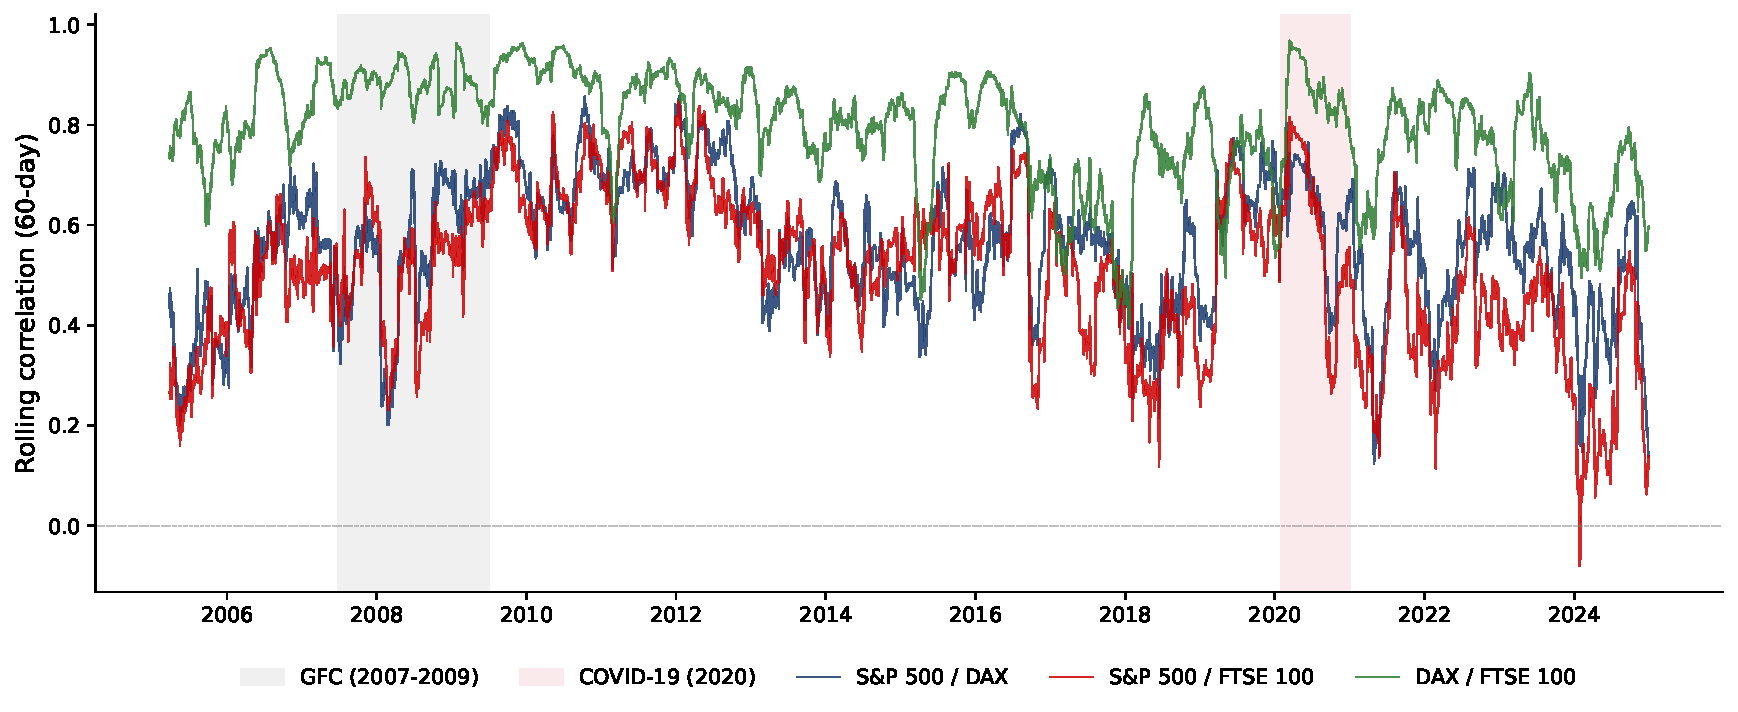
\includegraphics[width=0.95\textwidth, height=0.72\textheight, keepaspectratio]{../../charts/ch5b_rolling_correlations.pdf}
        \end{center}
    \end{cminipage}
    \hfill\quantlet{TSA\_ch5b\_rolling\_corr}{https://github.com/QuantLet/TSA/tree/main/TSA\_ch5b/TSA\_ch5b\_rolling\_corr}
\end{frame}

\begin{frame}{Correlation Distribution: Crisis vs.\ Calm Regimes}
    \begin{cminipage}{0.95\textwidth}
    \vspace{-2mm}
        \begin{center}
            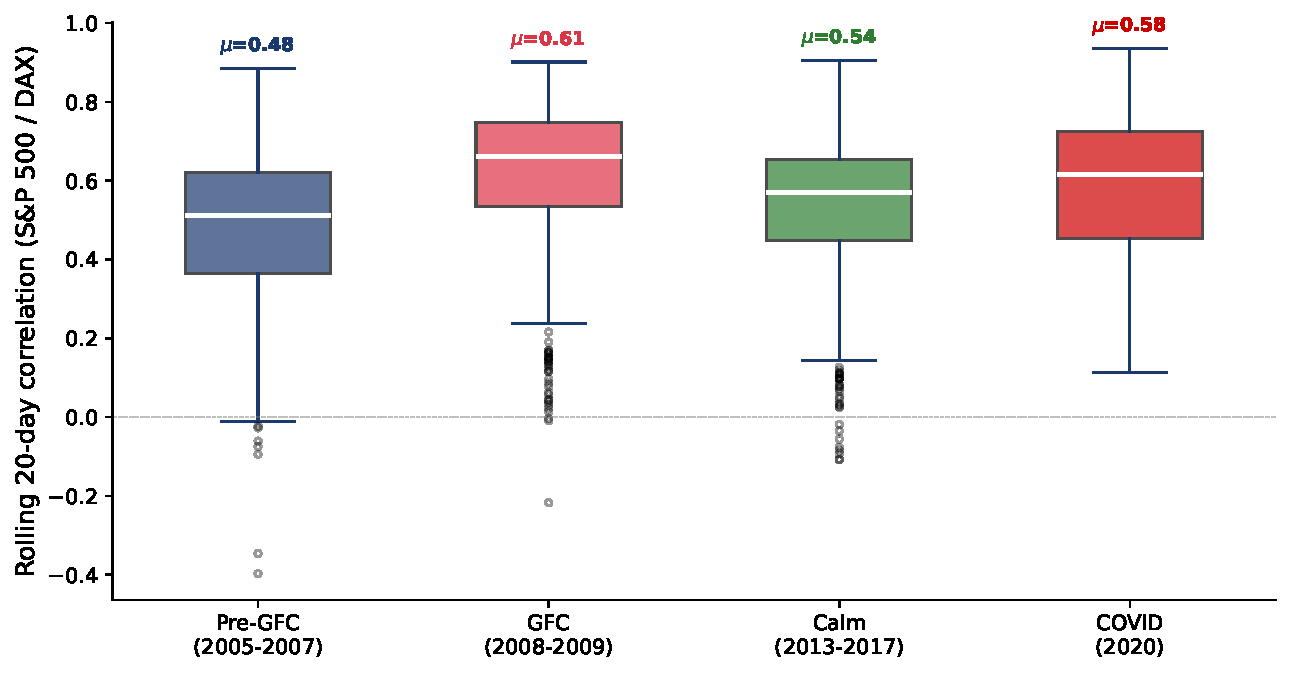
\includegraphics[width=0.85\textwidth, height=0.58\textheight, keepaspectratio]{../../charts/ch5b_crisis_boxplot.pdf}
        \end{center}
    \vspace{-3mm}
    {\footnotesize
    \begin{alertblock}{Key Observations}
        \begin{itemize}\setlength{\itemsep}{0pt}
            \item Median correlation increases significantly during crisis periods (GFC (\textit{Global Financial Crisis}), COVID)
            \item Correlation dispersion rises --- more uncertainty in cross-market relationships
        \end{itemize}
    \end{alertblock}
    }
    \end{cminipage}
    \hfill\quantlet{TSA\_ch5b\_crisis\_boxplot}{https://github.com/QuantLet/TSA/tree/main/TSA\_ch5b/TSA\_ch5b\_crisis\_boxplot}
\end{frame}

%=============================================================================
% SECTION 2: THE MULTIVARIATE GARCH FRAMEWORK
%=============================================================================
\section{The Multivariate GARCH Framework}

\begin{frame}{Half-Vectorization --- the $\text{vech}(\cdot)$ Operator}
    \begin{cminipage}{0.95\textwidth}
    \vspace{-3mm}
    {\footnotesize
    \begin{block}{Definition}
        \begin{itemize}\setlength{\itemsep}{0pt}
            \item The operator $\text{vech}: \mathbb{R}^{N \times N} \to \mathbb{R}^{N^*}$ stacks \textbf{column by column} the elements on and below the main diagonal of a symmetric matrix
            \item Output dimension: $N^* = N(N+1)/2$
            \item $\mathbf{H}_t$ is \textbf{symmetric}: $h_{ij,t} = h_{ji,t}$ --- $\text{vech}$ removes the $N(N-1)/2$ redundant elements
        \end{itemize}
        \[
            \mathbf{H}_t = \begin{pmatrix} h_{11,t} & \textcolor{MediumGray}{h_{12,t}} & \textcolor{MediumGray}{h_{13,t}} \\ h_{12,t} & h_{22,t} & \textcolor{MediumGray}{h_{23,t}} \\ h_{13,t} & h_{23,t} & h_{33,t} \end{pmatrix} \xrightarrow{\text{vech}} \begin{pmatrix} h_{11,t} \\ h_{12,t} \\ h_{13,t} \\ h_{22,t} \\ h_{23,t} \\ h_{33,t} \end{pmatrix}
        \]
        \vspace{-2mm}
        \begin{itemize}\setlength{\itemsep}{0pt}
            \item {\small Elements in \textcolor{MediumGray}{gray} are duplicates --- $\text{vech}$ removes them.}
        \end{itemize}
    \end{block}
    \begin{alertblock}{Central Role in Multivariate GARCH}
        \begin{itemize}\setlength{\itemsep}{0pt}
            \item Allows writing the model as a vector equation: $\text{vech}(\mathbf{H}_t) = \mathbf{c} + \mathbf{A}\,\text{vech}(\boldsymbol{\varepsilon}_{t-1}\boldsymbol{\varepsilon}_{t-1}') + \mathbf{B}\,\text{vech}(\mathbf{H}_{t-1})$
            \item Dimension: $N^*\!=\!N(N\!+\!1)/2$ --- for $N\!=\!2$: 3 elements; $N\!=\!10$: 55; $N\!=\!100$: 5,050
        \end{itemize}
    \end{alertblock}
    }
    \end{cminipage}
\end{frame}

\begin{frame}{General Setup}
    \begin{cminipage}{0.95\textwidth}
    {\footnotesize
    \begin{block}{Multivariate Return Process}
        \begin{itemize}\setlength{\itemsep}{0pt}
            \item $\mathbf{r}_t = (r_{1t}, \ldots, r_{Nt})'$: $N$-dimensional return vector
        \end{itemize}
        \vspace{-2mm}
        \begin{align}
            \mathbf{r}_t &= \boldsymbol{\mu}_t + \boldsymbol{\varepsilon}_t \\
            \boldsymbol{\varepsilon}_t &= \mathbf{H}_t^{1/2} \mathbf{z}_t, \qquad \mathbf{z}_t \overset{iid}{\sim} \mathcal{N}(\mathbf{0}, \mathbf{I}_N)
        \end{align}
        \vspace{-2mm}
        \begin{itemize}\setlength{\itemsep}{0pt}
            \item $\boldsymbol{\mu}_t$ = conditional mean vector (often a VAR or constant)
            \item $\mathbf{H}_t = \text{Var}(\boldsymbol{\varepsilon}_t \mid \mathcal{F}_{t-1})$ = $N \times N$ conditional covariance matrix
            \item $\mathbf{H}_t^{1/2}$ = any matrix square root such that $\mathbf{H}_t^{1/2}(\mathbf{H}_t^{1/2})' = \mathbf{H}_t$
        \end{itemize}
        \textit{Intuition: $\mathbf{H}_t^{1/2}\mathbf{z}_t$ transforms independent shocks into correlated returns --- the ``square root'' imprints the dependence structure.}
    \end{block}
    \begin{alertblock}{The Challenge}
        \begin{itemize}\setlength{\itemsep}{0pt}
            \item $\mathbf{H}_t$ has $N(N+1)/2$ unique elements. For $N=50$: \textbf{1,275 time-varying parameters} at each $t$!
        \end{itemize}
    \end{alertblock}
    }
    \end{cminipage}
\end{frame}

\begin{frame}{Positive Definiteness Requirement}
    \begin{cminipage}{0.95\textwidth}
    {\footnotesize
    \begin{block}{Why Positive Definiteness Matters}
        \begin{itemize}\setlength{\itemsep}{0pt}
            \item The conditional covariance matrix $\mathbf{H}_t$ must be \textbf{positive definite} (p.d.) for all $t$:
            \item Portfolio variance: $\sigma_p^2 = \mathbf{w}'\mathbf{H}_t\mathbf{w} > 0$ for all $\mathbf{w} \neq \mathbf{0}$
            \item The log-likelihood involves $\log|\mathbf{H}_t|$ and $\mathbf{H}_t^{-1}$ --- both require p.d.
            \item Cholesky decomposition for simulation requires p.d.
        \end{itemize}
    \end{block}
    \vspace{0.1cm}
    \begin{block}{Strategies to Ensure Positive Definiteness}
        \begin{enumerate}\setlength{\itemsep}{0pt}
            \item \textbf{Restrict parameters} so that $\mathbf{H}_t$ is p.d.\ by construction (BEKK)
            \item \textbf{Decompose} $\mathbf{H}_t = \mathbf{D}_t \mathbf{R}_t \mathbf{D}_t$ and model $\mathbf{D}_t$, $\mathbf{R}_t$ separately (DCC)
            \item \textbf{Work in factor space} to reduce dimensionality (Factor GARCH, GO-GARCH)
        \end{enumerate}
    \end{block}
    }
    \end{cminipage}
\end{frame}

\begin{frame}{The Cholesky Decomposition}
    \begin{cminipage}{0.95\textwidth}
    \vspace{-2mm}
    {\scriptsize
    \begin{block}{Definition}
        \begin{itemize}\setlength{\itemsep}{0pt}
            \item Any \textbf{symmetric positive definite} matrix $\mathbf{H}$ ($N \times N$) admits a \textbf{unique factorization}: $\mathbf{H} = \mathbf{L}\mathbf{L}'$
            \item $\mathbf{L}$ is a \textbf{lower triangular} matrix with \textbf{strictly positive} diagonal elements
            \item Complexity: $O(N^3/3)$ --- \textbf{twice as fast} as direct inversion
        \end{itemize}
    \end{block}
    \vspace{-1mm}
    \begin{block}{Example: the $2 \times 2$ case}
        \begin{itemize}\setlength{\itemsep}{0pt}
            \item Let $\mathbf{H} = \begin{pmatrix} h_{11} & h_{12} \\ h_{12} & h_{22} \end{pmatrix}$. Then $\mathbf{L} = \begin{pmatrix} \sqrt{h_{11}} & 0 \\ h_{12}/\sqrt{h_{11}} & \sqrt{h_{22} - h_{12}^2/h_{11}} \end{pmatrix}$
        \end{itemize}
    \end{block}
    \vspace{-1mm}
    \begin{alertblock}{Role in Multivariate GARCH}
        \begin{itemize}\setlength{\itemsep}{0pt}
            \item \textbf{Simulation}: $\boldsymbol{\varepsilon}_t = \mathbf{L}_t \mathbf{z}_t$, where $\mathbf{z}_t \sim N(\mathbf{0}, \mathbf{I})$ --- generates correlated shocks
            \item \textbf{Log-likelihood}: $\log|\mathbf{H}_t| = 2\sum_i \log L_{ii}$ --- avoids direct determinant computation
            \item \textbf{Inversion}: solve $\mathbf{L}_t \mathbf{x} = \boldsymbol{\varepsilon}_t$ by forward substitution ($O(N^2)$ vs.\ $O(N^3)$)
        \end{itemize}
    \end{alertblock}
    }
    \end{cminipage}
\end{frame}

\begin{frame}{Parameter Proliferation: The Curse of Dimensionality}
    \begin{cminipage}{0.95\textwidth}
    {\footnotesize
    \begin{block}{Number of Parameters by Model}
        \vspace{0.1cm}
        \begin{center}
        \begin{tabular}{lcc}
            \hline
            \textbf{Model} & \textbf{Parameters} & \textbf{$N=5$} \\
            \hline
            VEC(1,1) & $N(N+1)/2 + 2[N(N+1)/2]^2$ & 465 \\
            Diagonal VEC(1,1) & $3 \times N(N+1)/2$ & 45 \\
            BEKK(1,1) & $N(N+1)/2 + 2N^2$ & 65 \\
            Diagonal BEKK(1,1) & $N(N+1)/2 + 2N$ & 25 \\
            CCC(1,1) & $3N + N(N-1)/2$ & 25 \\
            DCC(1,1) & $3N + N(N-1)/2 + 2$ & 27 \\
            \hline
        \end{tabular}
        \end{center}
    \end{block}
    \vspace{0.1cm}
    \begin{alertblock}{Practical Implication}
        \begin{itemize}\setlength{\itemsep}{0pt}
            \item For large $N$, only \textbf{heavily parameterized models} (CCC, DCC, scalar BEKK, factor models) are feasible. Full VEC/BEKK become computationally intractable for $N > 5$.
        \end{itemize}
    \end{alertblock}
    }
    \end{cminipage}
\end{frame}

\begin{frame}{Curse of Dimensionality: Visualization}
    \begin{cminipage}{0.95\textwidth}
        \begin{center}
            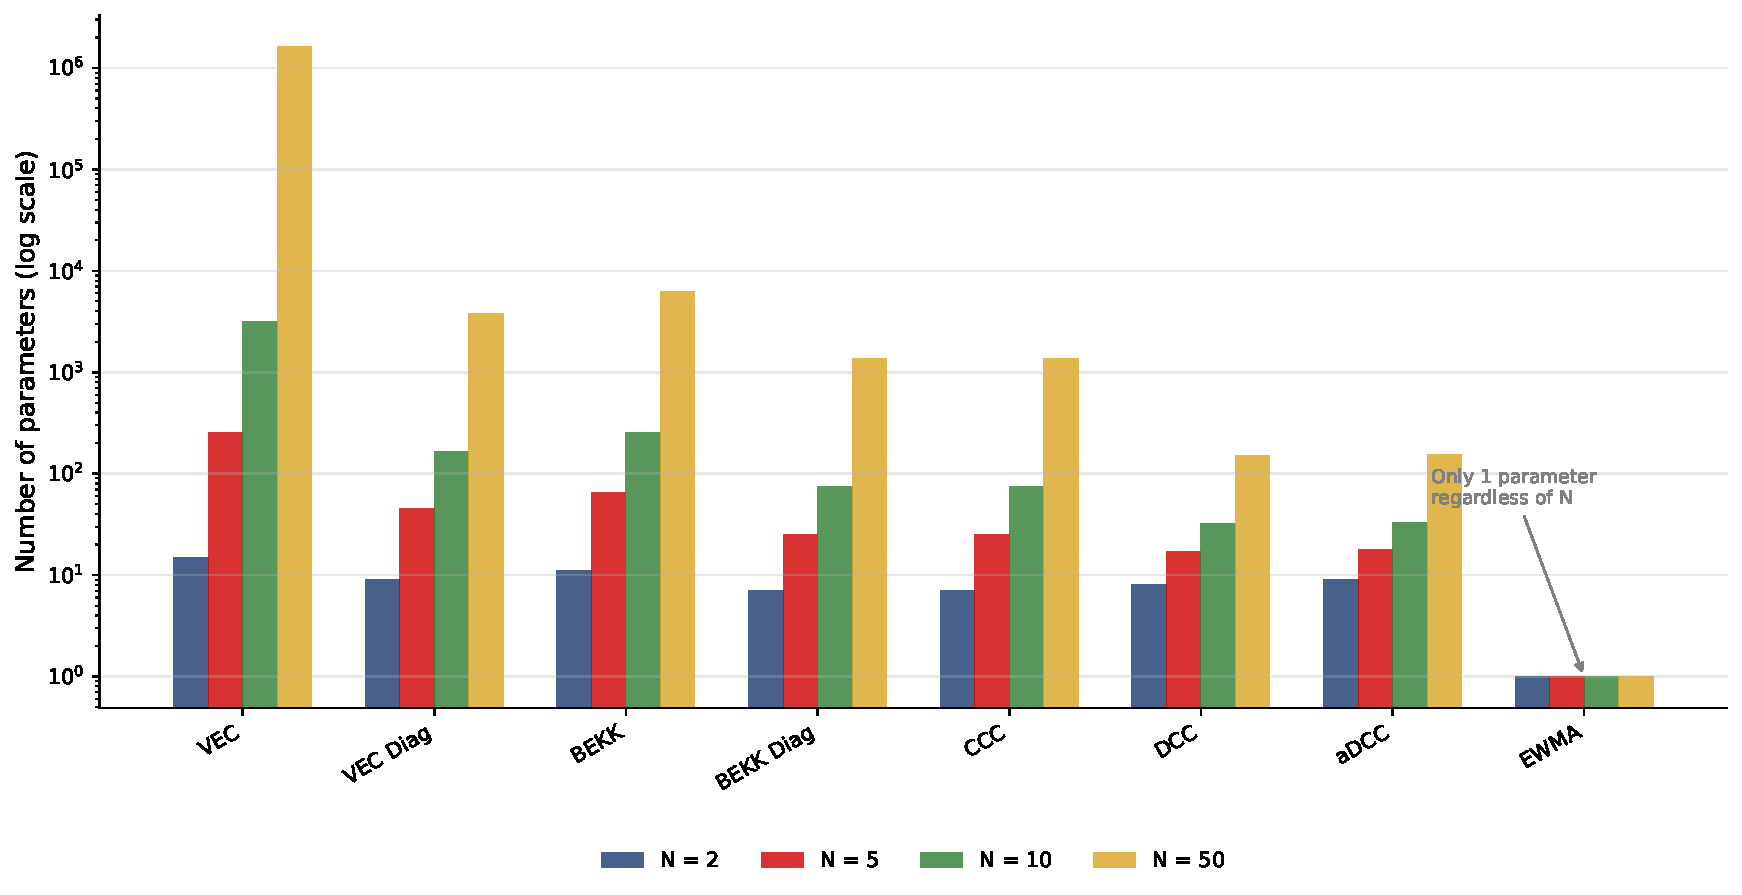
\includegraphics[width=0.92\textwidth, height=0.72\textheight, keepaspectratio]{../../charts/ch5b_param_comparison.pdf}
        \end{center}
    \end{cminipage}
    \hfill\quantlet{TSA\_ch5b\_param\_comparison}{https://github.com/QuantLet/TSA/tree/main/TSA\_ch5b/TSA\_ch5b\_param\_comparison}
\end{frame}

\begin{frame}{The Multivariate Normal Log-Likelihood}
    \begin{cminipage}{0.95\textwidth}
    {\footnotesize
    \begin{block}{General Log-Likelihood}
        \begin{itemize}\setlength{\itemsep}{0pt}
            \item For $T$ observations of $N$-dimensional returns:
        \end{itemize}
        \[
            \mathcal{L}(\boldsymbol{\theta}) = -\frac{TN}{2}\log(2\pi) - \frac{1}{2}\sum_{t=1}^T \left[ \underbrace{\log|\mathbf{H}_t|}_{\text{volume penalty}} + \underbrace{\boldsymbol{\varepsilon}_t'\mathbf{H}_t^{-1}\boldsymbol{\varepsilon}_t}_{\text{Mahalanobis distance}} \right]
        \]
        \textit{Intuition: the likelihood penalizes both large covariance (``diffuse forecast'') and large standardized residuals (``bad forecast'').}
    \end{block}
    \begin{block}{Computational Challenges}
        \begin{itemize}\setlength{\itemsep}{0pt}
            \item At each $t$: compute $\mathbf{H}_t$ ($O(N^2)$ or more), its inverse ($O(N^3)$), and determinant ($O(N^3)$)
            \item \textbf{Cholesky trick}: if $\mathbf{H}_t = \mathbf{L}_t\mathbf{L}_t'$, then $\log|\mathbf{H}_t| = 2\sum_{i}\log L_{ii}$ and solve $\mathbf{L}_t\mathbf{x} = \boldsymbol{\varepsilon}_t$ by forward substitution
            \item For DCC: two-step estimation dramatically reduces cost
        \end{itemize}
    \end{block}
    }
    \end{cminipage}
\end{frame}

%=============================================================================
% SECTION 3: VEC AND DIAGONAL VEC
%=============================================================================
\section{VEC and Diagonal VEC Models}

\begin{frame}{The VEC Model --- ``Mother'' of All MGARCH Models}
    \begin{cminipage}{0.95\textwidth}
    {\footnotesize
    \begin{block}{\textcolor{MainBlue}{Core Idea}: the most general linear MGARCH}
        \begin{itemize}\setlength{\itemsep}{0pt}
            \item Every model you will learn (BEKK, CCC, DCC) is a \textbf{restricted version} of VEC
            \item The VEC(1,1) equation:
        \end{itemize}
        \vspace{-2mm}
        \[
            \text{vech}(\mathbf{H}_t) = \underbrace{\mathbf{c}}_{\text{intercept}} + \underbrace{\mathbf{A}\,\text{vech}(\boldsymbol{\varepsilon}_{t-1}\boldsymbol{\varepsilon}_{t-1}')}_{\text{shock impact}} + \underbrace{\mathbf{B}\,\text{vech}(\mathbf{H}_{t-1})}_{\text{persistence}}
        \]
        \vspace{-2mm}
        \begin{itemize}\setlength{\itemsep}{0pt}
            \item $\mathbf{c}$: $N^* \times 1$; $\mathbf{A}, \mathbf{B}$: $N^* \times N^*$; $N^* = N(N+1)/2$
            \item Full $\mathbf{A}$ allows every shock to affect every covariance element
        \end{itemize}
        \textit{Intuition: today's covariance = baseline + yesterday's shocks + yesterday's covariance.}
    \end{block}
    \vspace{0.1cm}
    \begin{block}{Diagonal VEC: a Tractable Restriction}
        \begin{itemize}\setlength{\itemsep}{0pt}
            \item $\text{vech}(\mathbf{H}_t) = \mathbf{c} + \mathbf{a} \odot \text{vech}(\boldsymbol{\varepsilon}_{t-1}\boldsymbol{\varepsilon}_{t-1}') + \mathbf{b} \odot \text{vech}(\mathbf{H}_{t-1})$ \quad ($\odot$ = element-wise)
            \item Each variance/covariance follows its own GARCH --- \textbf{no cross-effects}
            \item Reduces parameters from $O(N^4)$ to $3N^*$
        \end{itemize}
    \end{block}
    }
    \end{cminipage}
\end{frame}

\begin{frame}{VEC: Limitations and Why We Move On}
    \begin{cminipage}{0.95\textwidth}
    {\footnotesize
    \textcolor{Crimson}{$\blacktriangleright$ \textbf{Limitation}: VEC is practically unusable for $N > 2$}
        \begin{itemize}\setlength{\itemsep}{0pt}
            \item For $N=3$: $\mathbf{A}$ is $6 \times 6$ $\Rightarrow$ \textbf{78 parameters}; for $N=5$: \textbf{465 parameters}
            \item \textbf{No guarantee} that $\mathbf{H}_t$ is positive definite
            \item Diagonal VEC reduces parameters but \textbf{kills all volatility spillovers}
        \end{itemize}
    \vspace{1mm}
    \textcolor{Forest}{$\blacktriangleright$ \textbf{When NOT to use VEC}}
        \begin{itemize}\setlength{\itemsep}{0pt}
            \item \textbf{Never} use full VEC for $N > 2$ --- estimation diverges
            \item \textbf{Avoid} Diagonal VEC for contagion studies --- it cannot capture spillovers
            \item \textbf{Skip} VEC entirely if you need guaranteed positive definiteness
        \end{itemize}
    \vspace{1mm}
    \textcolor{MainBlue}{\textbf{Model Positioning}}
        \begin{itemize}\setlength{\itemsep}{0pt}
            \item \textbf{Use when}: $N = 2$ and maximum flexibility is needed
            \item \textbf{vs.\ BEKK}: BEKK guarantees p.d.\ with same expressiveness --- prefer BEKK
        \end{itemize}
    \vspace{2mm}
    \textit{\textbf{Key takeaway:} VEC is the theoretical foundation --- but in practice, we need something better.}
    }
    \end{cminipage}
\end{frame}

%=============================================================================
% TRANSITION: VEC → BEKK
%=============================================================================

\begin{frame}{From VEC to BEKK: Why We Need Guaranteed Positive Definiteness}
    \begin{cminipage}{0.95\textwidth}
    \vspace{-2mm}
    {\scriptsize
    \begin{block}{What went wrong with VEC?}
        \begin{itemize}\setlength{\itemsep}{0pt}
            \item VEC is the most \textbf{general} multivariate GARCH --- every element of $\mathbf{H}_t$ has its own dynamics
            \item But: (1) \textbf{no guarantee} that $\mathbf{H}_t$ is positive definite, (2) parameter count \textbf{explodes} ($O(N^4)$)
            \item Diagonal VEC solves (2) but still fails at (1) --- and loses spillover effects
        \end{itemize}
    \end{block}
    \vspace{-2mm}
    \begin{alertblock}{The Core Problem}
        \begin{itemize}\setlength{\itemsep}{0pt}
            \item VEC writes $\text{vech}(\mathbf{H}_t) = \mathbf{c} + \mathbf{A}\,\text{vech}(\boldsymbol{\varepsilon}_{t-1}\boldsymbol{\varepsilon}_{t-1}') + \mathbf{B}\,\text{vech}(\mathbf{H}_{t-1})$
            \item Nothing in this equation \textbf{forces} $\mathbf{H}_t$ to be p.d.\ at every $t$
            \item Sufficient conditions exist (Engle \& Kroner, 1995) but are \textbf{hard to impose} during numerical optimization
        \end{itemize}
    \end{alertblock}
    \vspace{-2mm}
    \begin{exampleblock}{BEKK's Insight: Build PD Into the Structure}
        \begin{itemize}\setlength{\itemsep}{0pt}
            \item Write $\mathbf{H}_t = \mathbf{C}\mathbf{C}' + \mathbf{A}'\boldsymbol{\varepsilon}_{t-1}\boldsymbol{\varepsilon}_{t-1}'\mathbf{A} + \mathbf{B}'\mathbf{H}_{t-1}\mathbf{B}$
            \item Each term is p.s.d.\ \textbf{by construction} ($\mathbf{X}'\mathbf{M}\mathbf{X} \succeq 0$ for any $\mathbf{M} \succeq 0$)
            \item Sum of p.s.d.\ matrices + a p.d.\ matrix = p.d.\ always
        \end{itemize}
    \end{exampleblock}
    }
    \end{cminipage}
\end{frame}

%=============================================================================
% SECTION 4: THE BEKK MODEL
%=============================================================================
\section{The BEKK Model}

\begin{frame}{The BEKK Model (Engle \& Kroner, 1995)}
    \begin{cminipage}{0.95\textwidth}
    \vspace{-2mm}
    {\scriptsize
    \begin{block}{Definition: BEKK(1,1)}
        \[
            \mathbf{H}_t = \underbrace{\mathbf{C}\mathbf{C}'}_{\text{intercept (p.d.)}} + \underbrace{\mathbf{A}'\boldsymbol{\varepsilon}_{t-1}\boldsymbol{\varepsilon}_{t-1}'\mathbf{A}}_{\text{shock impact (p.s.d.)}} + \underbrace{\mathbf{B}'\mathbf{H}_{t-1}\mathbf{B}}_{\text{persistence (p.s.d.)}}
        \]
        \vspace{-2mm}
        \begin{itemize}\setlength{\itemsep}{0pt}
            \item $\mathbf{C}$: $N \times N$ lower triangular; $\mathbf{A}, \mathbf{B}$: $N \times N$ matrices
        \end{itemize}
        \textit{Intuition: the quadratic form $\mathbf{A}'\mathbf{M}\mathbf{A}$ is always p.s.d. --- positive definiteness comes ``for free.''}
    \end{block}
    \vspace{-1mm}
    \begin{block}{Key Properties}
        \begin{itemize}\setlength{\itemsep}{0pt}
            \item $\mathbf{H}_t$ is \textbf{positive definite by construction} (if $\mathbf{C}\mathbf{C}'$ is p.d.)
            \item Captures both \textbf{own-volatility persistence} and \textbf{cross-volatility spillovers}
            \item Parameters: $N(N+1)/2 + 2N^2$ --- for $N=3$: $6 + 18 = 24$
        \end{itemize}
    \end{block}
    \vspace{-1mm}
    \begin{alertblock}{\textcolor{Crimson}{$\blacktriangleright$ Practical Warning}: BEKK does not scale}
        \begin{itemize}\setlength{\itemsep}{0pt}
            \item Conceptually important, but \textbf{infeasible for $N > 5$} (parameter explosion: $2N^2$)
            \item BEKK = \textbf{B}aba, \textbf{E}ngle, \textbf{K}raft, \textbf{K}roner (1990)
        \end{itemize}
    \end{alertblock}
    }
    \end{cminipage}
\end{frame}

\begin{frame}{BEKK: Bivariate Case}
    \begin{cminipage}{0.95\textwidth}
    {\scriptsize
    \begin{block}{Expanding the BEKK(1,1) for $N=2$}
        \begin{itemize}\setlength{\itemsep}{0pt}
            \item Let $\mathbf{A} = \begin{pmatrix} a_{11} & a_{12} \\ a_{21} & a_{22} \end{pmatrix}$, $\mathbf{B} = \begin{pmatrix} b_{11} & b_{12} \\ b_{21} & b_{22} \end{pmatrix}$, $\mathbf{C} = \begin{pmatrix} c_{11} & 0 \\ c_{21} & c_{22} \end{pmatrix}$. Then:
        \end{itemize}
        \begin{align}
            h_{11,t} &= c_{11}^2 + a_{11}^2\varepsilon_{1,t-1}^2 + 2a_{11}a_{21}\varepsilon_{1,t-1}\varepsilon_{2,t-1} + a_{21}^2\varepsilon_{2,t-1}^2 \\
            &\quad + b_{11}^2 h_{11,t-1} + 2b_{11}b_{21}h_{12,t-1} + b_{21}^2 h_{22,t-1} \nonumber \\[3pt]
            h_{12,t} &= c_{11}c_{21} + a_{11}a_{12}\varepsilon_{1,t-1}^2 + (a_{11}a_{22}+a_{12}a_{21})\varepsilon_{1,t-1}\varepsilon_{2,t-1} + a_{21}a_{22}\varepsilon_{2,t-1}^2 \\
            &\quad + b_{11}b_{12}h_{11,t-1} + (b_{11}b_{22}+b_{12}b_{21})h_{12,t-1} + b_{21}b_{22}h_{22,t-1} \nonumber \\[3pt]
            h_{22,t} &= c_{21}^2 + c_{22}^2 + a_{12}^2\varepsilon_{1,t-1}^2 + 2a_{12}a_{22}\varepsilon_{1,t-1}\varepsilon_{2,t-1} + a_{22}^2\varepsilon_{2,t-1}^2 \\
            &\quad + b_{12}^2 h_{11,t-1} + 2b_{12}b_{22}h_{12,t-1} + b_{22}^2 h_{22,t-1} \nonumber
        \end{align}
    \end{block}
    \begin{alertblock}{Interpretation}
        \begin{itemize}\setlength{\itemsep}{0pt}
            \item Cross terms like $a_{21}^2\varepsilon_{2,t-1}^2$ in $h_{11,t}$: shock in asset 2 affects asset 1's variance = \textbf{volatility spillover}.
        \end{itemize}
    \end{alertblock}
    }
    \end{cminipage}
\end{frame}

\begin{frame}{Diagonal and Scalar BEKK}
    \begin{cminipage}{0.95\textwidth}
    \vspace{-2mm}
    {\scriptsize
    \begin{block}{Diagonal BEKK}
        \begin{itemize}\setlength{\itemsep}{0pt}
            \item Restrict $\mathbf{A}$ and $\mathbf{B}$ to be \textbf{diagonal}:
        \end{itemize}
        \[
            \mathbf{H}_t = \mathbf{C}\mathbf{C}' + \text{diag}(\mathbf{a})'\boldsymbol{\varepsilon}_{t-1}\boldsymbol{\varepsilon}_{t-1}'\text{diag}(\mathbf{a}) + \text{diag}(\mathbf{b})'\mathbf{H}_{t-1}\text{diag}(\mathbf{b})
        \]
        \begin{itemize}\setlength{\itemsep}{0pt}
            \item Parameters: $N(N+1)/2 + 2N$. Element-wise: $h_{ij,t} = c_{ij}^* + a_i a_j \varepsilon_{i,t-1}\varepsilon_{j,t-1} + b_i b_j h_{ij,t-1}$
        \end{itemize}
    \end{block}
    \vspace{-1mm}
    \begin{block}{Scalar BEKK}
        \begin{itemize}\setlength{\itemsep}{0pt}
            \item Further restrict: $\mathbf{A} = a\mathbf{I}_N$, $\mathbf{B} = b\mathbf{I}_N$:
        \end{itemize}
        \vspace{-2mm}
        \[
            \mathbf{H}_t = \mathbf{C}\mathbf{C}' + a^2\boldsymbol{\varepsilon}_{t-1}\boldsymbol{\varepsilon}_{t-1}' + b^2\mathbf{H}_{t-1}
        \]
        \vspace{-2mm}
        \begin{itemize}\setlength{\itemsep}{0pt}
            \item Parameters: $N(N+1)/2 + 2$. All pairs share the \textbf{same dynamics}.
        \end{itemize}
        \textit{Intuition: ``one knob for shock sensitivity, one for memory'' --- identical across all pairs.}
    \end{block}
    \vspace{-2mm}
    \begin{alertblock}{Trade-off}
        \begin{itemize}\setlength{\itemsep}{0pt}
            \item Diagonal/Scalar BEKK: feasible for large $N$, but \textbf{no cross-asset spillovers}.
        \end{itemize}
    \end{alertblock}
    }
    \end{cminipage}
\end{frame}

\begin{frame}{The Kronecker Product}
    \begin{cminipage}{0.95\textwidth}
    \vspace{-3mm}
    {\scriptsize
    \begin{block}{Definition}
        \begin{itemize}\setlength{\itemsep}{0pt}
            \item Let $\mathbf{A} \in \mathbb{R}^{m \times n}$ and $\mathbf{B} \in \mathbb{R}^{p \times q}$. The \textbf{Kronecker product} $\mathbf{A} \otimes \mathbf{B}$ is the $mp \times nq$ block matrix:
            \vspace{-1mm}
            \[
                \mathbf{A} \otimes \mathbf{B} = \begin{pmatrix} a_{11}\mathbf{B} & \cdots & a_{1n}\mathbf{B} \\ \vdots & \ddots & \vdots \\ a_{m1}\mathbf{B} & \cdots & a_{mn}\mathbf{B} \end{pmatrix}
            \]
            \vspace{-3mm}
            \item Dimensions do \textbf{not} need to match (unlike Hadamard)
        \end{itemize}
    \end{block}
    \vspace{-2mm}
    \begin{block}{Example: $2 \times 2$}
        \vspace{-2mm}
        \[
            \begin{pmatrix} a & b \\ c & d \end{pmatrix} \otimes \begin{pmatrix} e & f \\ g & h \end{pmatrix} = \begin{pmatrix} ae & af & be & bf \\ ag & ah & bg & bh \\ ce & cf & de & df \\ cg & ch & dg & dh \end{pmatrix} \quad \text{(result is } 4 \times 4\text{)}
        \]
        \vspace{-3mm}
    \end{block}
    \vspace{-2mm}
    \begin{alertblock}{Role in Multivariate GARCH}
        \begin{itemize}\setlength{\itemsep}{0pt}
            \item BEKK stationarity condition: $\rho(\mathbf{A} \otimes \mathbf{A} + \mathbf{B} \otimes \mathbf{B}) < 1$
            \item Unconditional covariance: $\text{vech}(\bar{\mathbf{H}}) = (\mathbf{I} - \mathbf{A} \otimes \mathbf{A} - \mathbf{B} \otimes \mathbf{B})^{-1}\text{vech}(\mathbf{C}\mathbf{C}')$
        \end{itemize}
    \end{alertblock}
    }
    \end{cminipage}
\end{frame}

\begin{frame}{BEKK: Stationarity and Unconditional Covariance}
    \begin{cminipage}{0.95\textwidth}
    {\footnotesize
    \begin{block}{Stationarity Condition}
        \begin{itemize}\setlength{\itemsep}{0pt}
            \item The BEKK(1,1) process is covariance stationary if and only if:
        \end{itemize}
        \[
            \rho(\mathbf{A} \otimes \mathbf{A} + \mathbf{B} \otimes \mathbf{B}) < 1
        \]
        \begin{itemize}\setlength{\itemsep}{0pt}
            \item where $\rho(\cdot)$ denotes the spectral radius and $\otimes$ is the Kronecker product
        \end{itemize}
        \textit{Intuition: the multivariate analogue of $\alpha + \beta < 1$ --- shocks must decay, not explode.}
    \end{block}
    \vspace{0.1cm}
    \begin{block}{Unconditional Covariance Matrix}
        \begin{itemize}\setlength{\itemsep}{0pt}
            \item If the stationarity condition holds:
        \end{itemize}
        \[
            \text{vech}(\bar{\mathbf{H}}) = (\mathbf{I}_{N^*} - \mathbf{A} \otimes \mathbf{A} - \mathbf{B} \otimes \mathbf{B})^{-1} \text{vech}(\mathbf{C}\mathbf{C}')
        \]
        \textit{Intuition: the long-run covariance matrix that $\mathbf{H}_t$ gravitates toward --- like $\bar{\sigma}^2 = \omega/(1-\alpha-\beta)$ in univariate GARCH.}
    \end{block}
    }
    \end{cminipage}
\end{frame}

\begin{frame}{BEKK: Strengths, Weaknesses, and Variant Selection}
    \begin{cminipage}{0.95\textwidth}
    \vspace{-3mm}
    {\scriptsize
    \begin{block}{Strengths}
        \begin{itemize}\setlength{\itemsep}{0pt}
            \item \textbf{Positive definiteness by construction} --- no additional restrictions needed
            \item Captures \textbf{volatility spillovers} --- the only class that directly models them
            \item Direct interpretation of $\mathbf{A}$ and $\mathbf{B}$: shock transmission and persistence
        \end{itemize}
    \end{block}
    \begin{alertblock}{Weaknesses}
        \begin{itemize}\setlength{\itemsep}{0pt}
            \item \textbf{Parameter explosion}: full BEKK for $N=10$ $\Rightarrow$ 255 parameters
            \item Numerically \textbf{unstable} optimization --- multiple local optima, slow convergence
            \item Results can be \textbf{sensitive to starting values}
            \item Cannot be decomposed into stages --- joint estimation required
        \end{itemize}
    \end{alertblock}
    \begin{block}{Practical Rule}
        \begin{itemize}\setlength{\itemsep}{0pt}
            \item $N \leq 3$: full BEKK (if spillovers matter)
            \item $3 < N \leq 10$: diagonal BEKK
            \item $N > 10$: switch to DCC or factor models
        \end{itemize}
    \end{block}
    }
    \end{cminipage}
\end{frame}

%=============================================================================
% BEKK: KEY INSIGHT + PITFALL
%=============================================================================

\begin{frame}{BEKK: Key Insight and Common Pitfalls}
    \begin{cminipage}{0.95\textwidth}
    \vspace{-4mm}
    {\scriptsize
    \begin{block}{\textcolor{MainBlue}{$\blacktriangleright$ Key Insight}: BEKK is a ``smart reparametrization'' of VEC}
        \begin{itemize}\setlength{\itemsep}{0pt}
            \item BEKK does not add new economics --- it writes the \textit{same} dynamics in a p.d.-guaranteed form
            \item $\mathbf{A}'\mathbf{M}\mathbf{A}$ is p.s.d.\ by linear algebra, not economic theory; trades flexibility for convenience
        \end{itemize}
    \end{block}
    \vspace{-2mm}
    \begin{alertblock}{\textcolor{Crimson}{$\blacktriangleright$ Common Pitfall}: using full BEKK for $N > 5$}
        \begin{itemize}\setlength{\itemsep}{0pt}
            \item Full BEKK for $N = 10$: \textbf{255 parameters} --- optimizer finds local optima, results are fragile
            \item Caporin \& McAleer (2012): ``full BEKK is essentially uninterpretable for $N > 3$''
            \item Diagonal BEKK is often the practical choice, but then spillovers vanish --- defeating BEKK's purpose
        \end{itemize}
    \end{alertblock}
    \vspace{-2mm}
    \begin{exampleblock}{\textcolor{Forest}{$\blacktriangleright$ When NOT to use BEKK}}
        \begin{itemize}\setlength{\itemsep}{0pt}
            \item $N > 5$: use DCC or factor models instead
            \item When you don't care about \textit{direction} of spillovers (DCC captures co-movement without spillover channels)
            \item When you need fast re-estimation (BEKK: hours vs.\ DCC: seconds for $N = 50$)
        \end{itemize}
    \end{exampleblock}
    }
    \end{cminipage}
\end{frame}

\begin{frame}{BEKK Section Summary}
    \begin{cminipage}{0.95\textwidth}
    {\footnotesize
    \begin{block}{3 Things to Remember}
        \begin{enumerate}\setlength{\itemsep}{2pt}
            \item BEKK guarantees p.d.\ via the quadratic form $\mathbf{A}'\mathbf{M}\mathbf{A}$ --- the \textbf{only} model that directly captures spillovers
            \item Full BEKK: rich but infeasible for $N > 5$; diagonal BEKK: scalable but no spillovers
            \item Estimation requires joint optimization --- no two-step shortcut
        \end{enumerate}
    \end{block}
    \begin{alertblock}{Model Positioning}
        \begin{itemize}\setlength{\itemsep}{0pt}
            \item \textbf{Use when}: $N \leq 5$ and volatility spillover \textit{direction} matters
            \item \textbf{vs.\ VEC}: same flexibility, guaranteed p.d. \quad \textbf{vs.\ DCC}: DCC scales better but cannot identify spillover direction
        \end{itemize}
    \end{alertblock}
    }
    \end{cminipage}
\end{frame}

%=============================================================================
% TRANSITION: BEKK → CCC
%=============================================================================

\begin{frame}{From BEKK to CCC: The Decomposition That Changed Everything}
    \begin{cminipage}{0.95\textwidth}
    \vspace{-2mm}
    {\scriptsize
    \begin{block}{What BEKK taught us --- and where it breaks down}
        \begin{itemize}\setlength{\itemsep}{0pt}
            \item BEKK \textbf{solved} the PD problem and models volatility spillovers directly
            \item But: $N(N+1)/2 + 2N^2$ parameters $\Rightarrow$ estimation collapses for $N > 5$
            \item Joint estimation of all parameters --- no decomposition into simpler sub-problems
            \item \textcolor{Crimson}{Practitioners abandoned BEKK for large portfolios by the late 1990s}
        \end{itemize}
    \end{block}
    \vspace{-2mm}
    \begin{alertblock}{Bollerslev's Insight (1990): Separate What Changes from What Doesn't}
        \begin{itemize}\setlength{\itemsep}{0pt}
            \item \textbf{Observation}: variances change every day, but \textit{correlations} move slowly
            \item \textbf{Idea}: decompose $\mathbf{H}_t = \mathbf{D}_t \mathbf{R} \mathbf{D}_t$ where $\mathbf{D}_t$ varies but $\mathbf{R}$ is fixed
            \item This separates a \textbf{hard} joint problem into $N$ \textbf{easy} univariate problems + one correlation estimate
        \end{itemize}
    \end{alertblock}
    \vspace{-2mm}
    \begin{exampleblock}{The Trade-off}
        \begin{itemize}\setlength{\itemsep}{0pt}
            \item \textcolor{Forest}{Gained}: scalability ($3N + N(N-1)/2$ params), two-step estimation, handles $N > 100$
            \item \textcolor{Crimson}{Lost}: volatility spillovers, time-varying correlations (constant $\mathbf{R}$!)
            \item This trade-off motivated CCC --- and later DCC to restore dynamic correlations
        \end{itemize}
    \end{exampleblock}
    }
    \end{cminipage}
\end{frame}

%=============================================================================
% SECTION 5: CCC MODEL
%=============================================================================
\section{Constant Conditional Correlation (CCC)}

\begin{frame}{The CCC Model (Bollerslev, 1990)}
    \begin{cminipage}{0.95\textwidth}
    {\footnotesize
    \begin{block}{Key Idea: Separate Variances from Correlations}
        \begin{itemize}\setlength{\itemsep}{0pt}
            \item Decompose the conditional covariance matrix:
        \end{itemize}
        \[
            \mathbf{H}_t = \underbrace{\mathbf{D}_t}_{\text{volatilities}} \underbrace{\mathbf{R}}_{\text{correlations}} \underbrace{\mathbf{D}_t}_{\text{volatilities}}
        \]
        \begin{itemize}\setlength{\itemsep}{0pt}
            \item $\mathbf{D}_t = \text{diag}(\sqrt{h_{11,t}}, \ldots, \sqrt{h_{NN,t}})$ --- conditional standard deviations (time-varying)
            \item $\mathbf{R}$ --- \textbf{constant} correlation matrix (time-invariant)
            \item Each $h_{ii,t}$ follows a \textbf{univariate GARCH(1,1)}:
                $h_{ii,t} = \omega_i + \alpha_i \varepsilon_{i,t-1}^2 + \beta_i h_{ii,t-1}$
        \end{itemize}
        \textit{Intuition: covariances change only because volatilities change --- the ``wiring'' between assets stays fixed.}
    \end{block}
    \vspace{0.1cm}
    \begin{alertblock}{Properties}
        \begin{itemize}\setlength{\itemsep}{0pt}
            \item $\mathbf{H}_t$ is p.d.\ if and only if $\mathbf{R}$ is p.d.\ and all $h_{ii,t} > 0$
            \item Parameters: $3N + N(N-1)/2$ --- very parsimonious
            \item Covariances: $h_{ij,t} = \rho_{ij}\sqrt{h_{ii,t}}\sqrt{h_{jj,t}}$
        \end{itemize}
    \end{alertblock}
    }
    \end{cminipage}
\end{frame}

\begin{frame}{CCC: Two-Step Estimation}
    \begin{cminipage}{0.95\textwidth}
    \vspace{-3mm}
    {\scriptsize
    \begin{block}{Step 1: Estimate Univariate GARCH Models}
        \begin{itemize}\setlength{\itemsep}{0pt}
            \item For each asset $i = 1, \ldots, N$:
        \end{itemize}
        \begin{enumerate}\setlength{\itemsep}{0pt}
            \item Estimate a GARCH(1,1) model for $r_{it}$
            \item Obtain the standardized residuals: $z_{it} = \varepsilon_{it} / \sqrt{h_{ii,t}}$
        \end{enumerate}
    \end{block}
    \begin{block}{Step 2: Estimate the Correlation Matrix}
        \vspace{-1mm}
        \[
            \hat{\mathbf{R}} = \frac{1}{T}\sum_{t=1}^T \mathbf{z}_t\mathbf{z}_t'
        \]
        \vspace{-2mm}
        \begin{itemize}\setlength{\itemsep}{0pt}
            \item where $\mathbf{z}_t = (z_{1t}, \ldots, z_{Nt})'$ are the standardized residuals from Step 1
        \end{itemize}
    \end{block}
    \begin{alertblock}{Advantage}
        \begin{itemize}\setlength{\itemsep}{0pt}
            \item Each step involves \textbf{low-dimensional optimization}
            \item Step 1: $N$ univariate optimizations (3 params each); Step 2: sample correlation --- no optimization
        \end{itemize}
    \end{alertblock}
    }
    \end{cminipage}
\end{frame}

\begin{frame}{CCC: Strengths and Limitations}
    \begin{cminipage}{0.95\textwidth}
    {\footnotesize
    \begin{block}{Strengths}
        \begin{itemize}\setlength{\itemsep}{0pt}
            \item \textbf{Parsimony}: few parameters, easy to estimate even for large $N$
            \item \textbf{Positive definiteness}: guaranteed by construction
            \item \textbf{Interpretability}: time-varying covariances driven solely by changing variances
            \item Good \textbf{baseline model} for comparison
        \end{itemize}
    \end{block}
    \vspace{0.2cm}
    \begin{alertblock}{Limitations}
        \begin{itemize}\setlength{\itemsep}{0pt}
            \item \textbf{Constant correlations} are empirically rejected in most financial data
            \item Cannot capture \textbf{contagion} or \textbf{flight-to-quality} effects
            \item Covariances change only because variances change, not because the \textbf{relationship} between assets changes
            \item Tse (2000) and Engle (2002) proposed tests for constant correlation
        \end{itemize}
    \end{alertblock}
    }
    \end{cminipage}
\end{frame}

%=============================================================================
% CCC: KEY INSIGHT + PITFALL
%=============================================================================

\begin{frame}{CCC: Key Insight and Common Pitfalls}
    \begin{cminipage}{0.95\textwidth}
    \vspace{-4mm}
    {\scriptsize
    \begin{block}{\textcolor{MainBlue}{$\blacktriangleright$ Key Insight}: CCC made MGARCH practical --- not accurate}
        \begin{itemize}\setlength{\itemsep}{0pt}
            \item CCC's genius is \textbf{computational}: fixing $\mathbf{R}$ decomposes the problem into $N$ univariate GARCHs
            \item CCC is rarely the ``right'' model, but always the right \textbf{benchmark}
            \item If DCC cannot beat CCC out-of-sample, the extra complexity is wasted
        \end{itemize}
    \end{block}
    \vspace{-2mm}
    \begin{alertblock}{\textcolor{Crimson}{$\blacktriangleright$ Common Pitfall}: using CCC for risk management during crises}
        \begin{itemize}\setlength{\itemsep}{0pt}
            \item CCC \textbf{underestimates} portfolio VaR during stress: true correlations spike, but CCC uses the sample average
            \item Empirically: CCC underestimates crisis VaR by 20--30\% vs.\ DCC (see Case Study 1)
            \item Regulators (Basel III/IV) expect models to capture \textbf{time-varying} dependence
        \end{itemize}
    \end{alertblock}
    \vspace{-2mm}
    \begin{exampleblock}{\textcolor{Forest}{$\blacktriangleright$ When CCC is actually fine}}
        \begin{itemize}\setlength{\itemsep}{0pt}
            \item Short horizons (< 1 year) where correlations haven't changed much
            \item Asset pairs with genuinely stable correlations (e.g., same-sector stocks)
            \item As a \textbf{diagnostic tool}: if CCC and DCC give similar results, correlations are stable
        \end{itemize}
    \end{exampleblock}
    }
    \end{cminipage}
\end{frame}

\begin{frame}{CCC Section Summary}
    \begin{cminipage}{0.95\textwidth}
    {\footnotesize
    \begin{block}{3 Things to Remember}
        \begin{enumerate}\setlength{\itemsep}{2pt}
            \item CCC decomposes $\mathbf{H}_t = \mathbf{D}_t\mathbf{R}\mathbf{D}_t$ --- \textbf{variances move, correlations don't}
            \item Two-step estimation: $N$ univariate GARCHs + sample correlation --- fast, scalable, guaranteed p.d.
            \item Constant correlations are empirically \textbf{rejected} in most financial data
        \end{enumerate}
    \end{block}
    \begin{alertblock}{Model Positioning}
        \begin{itemize}\setlength{\itemsep}{0pt}
            \item \textbf{Use as}: the default \textbf{benchmark} --- if DCC can't beat it, complexity is wasted
            \item \textbf{vs.\ BEKK}: much simpler, no spillovers \quad \textbf{vs.\ DCC}: same structure, but $\mathbf{R}$ is fixed
        \end{itemize}
    \end{alertblock}
    }
    \end{cminipage}
\end{frame}

%=============================================================================
% TRANSITION: CCC → DCC
%=============================================================================

\begin{frame}{From CCC to DCC: When Correlations Must Move}
    \begin{cminipage}{0.95\textwidth}
    \vspace{-3mm}
    {\scriptsize
    \begin{block}{The empirical evidence against constant correlations}
        \begin{itemize}\setlength{\itemsep}{0pt}
            \item CCC assumes $\rho_{ij}$ is \textbf{fixed} --- but crises repeatedly violate this
            \item S\&P~500--DAX correlation: $\approx 0.40$ in calm markets, $> 0.85$ during GFC (2008)
            \item Stock--bond correlation \textbf{flipped sign}: $+0.30$ pre-2000 $\to$ $-0.30$ post-2000 (flight to quality)
            \item \textcolor{Crimson}{Tse (2000) and Engle--Sheppard (2001): constant correlation rejected at 1\% in most pairs}
        \end{itemize}
    \end{block}
    \vspace{-2mm}
    \begin{alertblock}{Engle's Solution (2002): Keep the $\mathbf{D}_t\mathbf{R}_t\mathbf{D}_t$ Structure, Make $\mathbf{R}_t$ Dynamic}
        \begin{itemize}\setlength{\itemsep}{0pt}
            \item Replace $\mathbf{R}$ with $\mathbf{R}_t$ --- correlations now respond to joint shocks
            \item Key trick: model a proxy $\mathbf{Q}_t$ (which is \textit{not} a correlation matrix), then rescale
            \item \textbf{Only 2 extra parameters} $(a, b)$ regardless of portfolio size $N$
        \end{itemize}
    \end{alertblock}
    \vspace{-2mm}
    \begin{exampleblock}{What DCC preserves from CCC}
        \begin{itemize}\setlength{\itemsep}{0pt}
            \item Same two-step estimation: Step~1 is identical (univariate GARCHs)
            \item Same scalability: $3N + N(N-1)/2 + 2$ parameters --- just 2 more than CCC
            \item If $a = b = 0$, DCC \textbf{reduces exactly to CCC} --- CCC is nested
        \end{itemize}
    \end{exampleblock}
    }
    \end{cminipage}
\end{frame}

%=============================================================================
% SECTION 6: DCC MODEL
%=============================================================================
\section{Dynamic Conditional Correlation (DCC)}

\begin{frame}{The DCC Model (Engle, 2002)}
    \begin{cminipage}{0.95\textwidth}
    {\footnotesize
    \begin{alertblock}{\textcolor{Crimson}{$\star$ Core Model}: DCC = CCC + dynamic correlations + only 2 extra parameters}
        \begin{itemize}\setlength{\itemsep}{0pt}
            \item Same decomposition: $\mathbf{H}_t = \mathbf{D}_t \mathbf{R}_t \mathbf{D}_t$
            \item Same $\mathbf{D}_t$ (univariate GARCH), but $\mathbf{R}_t$ is now \textbf{time-varying}
        \end{itemize}
    \end{alertblock}
    \vspace{0.1cm}
    \begin{block}{Correlation Dynamics (the only new equation)}
        \begin{itemize}\setlength{\itemsep}{0pt}
            \item $\mathbf{R}_t$ is derived from a pseudo-correlation matrix $\mathbf{Q}_t$:
        \end{itemize}
        \vspace{-2mm}
        \begin{align}
            \mathbf{Q}_t &= (1-a-b)\bar{\mathbf{Q}} + a\,\mathbf{z}_{t-1}\mathbf{z}_{t-1}' + b\,\mathbf{Q}_{t-1} \\
            \mathbf{R}_t &= \text{diag}(\mathbf{Q}_t)^{-1/2}\,\mathbf{Q}_t\,\text{diag}(\mathbf{Q}_t)^{-1/2}
        \end{align}
        \vspace{-2mm}
        \begin{itemize}\setlength{\itemsep}{0pt}
            \item $\bar{\mathbf{Q}}$: unconditional correlation; $a$: news impact; $b$: persistence; $a + b < 1$
        \end{itemize}
        \textit{Intuition: correlations spike when assets move together and mean-revert to $\bar{\mathbf{Q}}$ otherwise.}
    \end{block}
    }
    \end{cminipage}
\end{frame}

\begin{frame}{DCC: Intuition and Interpretation}
    \begin{cminipage}{0.95\textwidth}
    {\footnotesize
    \begin{block}{The $\mathbf{Q}_t$ Process}
        \[
            \mathbf{Q}_t = \underbrace{(1-a-b)\bar{\mathbf{Q}}}_{\text{mean reversion}} + \underbrace{a\,\mathbf{z}_{t-1}\mathbf{z}_{t-1}'}_{\text{news impact}} + \underbrace{b\,\mathbf{Q}_{t-1}}_{\text{persistence}}
        \]
        \begin{itemize}\setlength{\itemsep}{0pt}
            \item $a$ measures how \textbf{quickly correlations react} to new shocks
            \item $b$ measures the \textbf{persistence} of correlations
            \item $a + b$ close to 1: correlations are highly persistent (close to IGARCH-like behavior)
            \item If $a = b = 0$: DCC reduces to CCC
        \end{itemize}
    \end{block}
    \vspace{0.1cm}
    \begin{block}{The Rescaling Step}
        \begin{itemize}\setlength{\itemsep}{0pt}
            \item $\mathbf{Q}_t$ is \textbf{not} a proper correlation matrix (diagonal $\neq 1$)
            \item The rescaling $\mathbf{R}_t = \text{diag}(\mathbf{Q}_t)^{-1/2}\mathbf{Q}_t\,\text{diag}(\mathbf{Q}_t)^{-1/2}$ ensures $R_{ii,t} = 1$
            \item This guarantees $-1 \leq R_{ij,t} \leq 1$ and $\mathbf{R}_t$ is p.d.\ (if $\mathbf{Q}_t$ is p.d.)
        \end{itemize}
    \end{block}
    }
    \end{cminipage}
\end{frame}

\begin{frame}{DCC: Two-Step Estimation}
    \begin{cminipage}{0.95\textwidth}
    \vspace{-2mm}
    {\scriptsize
    \begin{block}{Step 1: Univariate GARCH (Same as CCC)}
        \begin{enumerate}\setlength{\itemsep}{0pt}
            \item Estimate GARCH(1,1) for each asset $i$ separately
            \item Compute standardized residuals $z_{it} = \varepsilon_{it}/\sqrt{h_{ii,t}}$
            \item Compute $\bar{\mathbf{Q}} = T^{-1}\sum_t \mathbf{z}_t\mathbf{z}_t'$
        \end{enumerate}
    \end{block}
    \vspace{-1mm}
    \begin{block}{Step 2: Estimate DCC Parameters $(a, b)$}
        \begin{itemize}\setlength{\itemsep}{0pt}
            \item Maximize the \textbf{correlation component} of the log-likelihood:
        \end{itemize}
        \vspace{-2mm}
        \[
            \mathcal{L}_2(a,b) = -\frac{1}{2}\sum_{t=1}^T \left[ \log|\mathbf{R}_t| + \mathbf{z}_t'\mathbf{R}_t^{-1}\mathbf{z}_t - \mathbf{z}_t'\mathbf{z}_t \right]
        \]
        \vspace{-3mm}
        \begin{itemize}\setlength{\itemsep}{0pt}
            \item A \textbf{2-parameter} optimization regardless of $N$!
        \end{itemize}
        \textit{Intuition: only the ``correlation part'' of the likelihood --- volatility was handled in Step 1.}
    \end{block}
    \vspace{-1mm}
    \begin{alertblock}{Composite Likelihood}
        \begin{itemize}\setlength{\itemsep}{0pt}
            \item Consistent but not fully efficient. SEs require Bollerslev--Wooldridge sandwich estimator.
        \end{itemize}
    \end{alertblock}
    }
    \end{cminipage}
\end{frame}

\begin{frame}{DCC: Bivariate Example}
    \begin{cminipage}{0.95\textwidth}
    {\footnotesize
    \begin{exampleblock}{Example: Two Assets ($N=2$)}
        \begin{itemize}\setlength{\itemsep}{0pt}
            \item With $\mathbf{z}_t = (z_{1t}, z_{2t})'$, the DCC dynamics simplify to:
        \end{itemize}
        \begin{align}
            q_{12,t} &= (1-a-b)\bar{q}_{12} + a\,z_{1,t-1}z_{2,t-1} + b\,q_{12,t-1} \\
            \rho_{12,t} &= \frac{q_{12,t}}{\sqrt{q_{11,t}\,q_{22,t}}}
        \end{align}
        \begin{itemize}\setlength{\itemsep}{0pt}
            \item where $q_{11,t} = (1-a-b) + a\,z_{1,t-1}^2 + b\,q_{11,t-1}$ (and similarly for $q_{22,t}$)
        \end{itemize}
    \end{exampleblock}
    \vspace{0.1cm}
    \begin{block}{Interpretation}
        \begin{itemize}\setlength{\itemsep}{0pt}
            \item If both $z_{1,t-1}$ and $z_{2,t-1}$ are large and have the \textbf{same sign}: $q_{12,t}$ increases $\Rightarrow$ correlation increases
            \item Joint negative shocks (crises) \textbf{push correlations upward} --- captures contagion
            \item Correlations \textbf{mean-revert} to $\bar{q}_{12}$ at rate $(1-a-b)$
        \end{itemize}
    \end{block}
    }
    \end{cminipage}
\end{frame}

\begin{frame}{Case Study: DCC vs.\ Rolling Correlation (S\&P 500 -- DAX)}
    \begin{cminipage}{0.95\textwidth}
        \begin{center}
            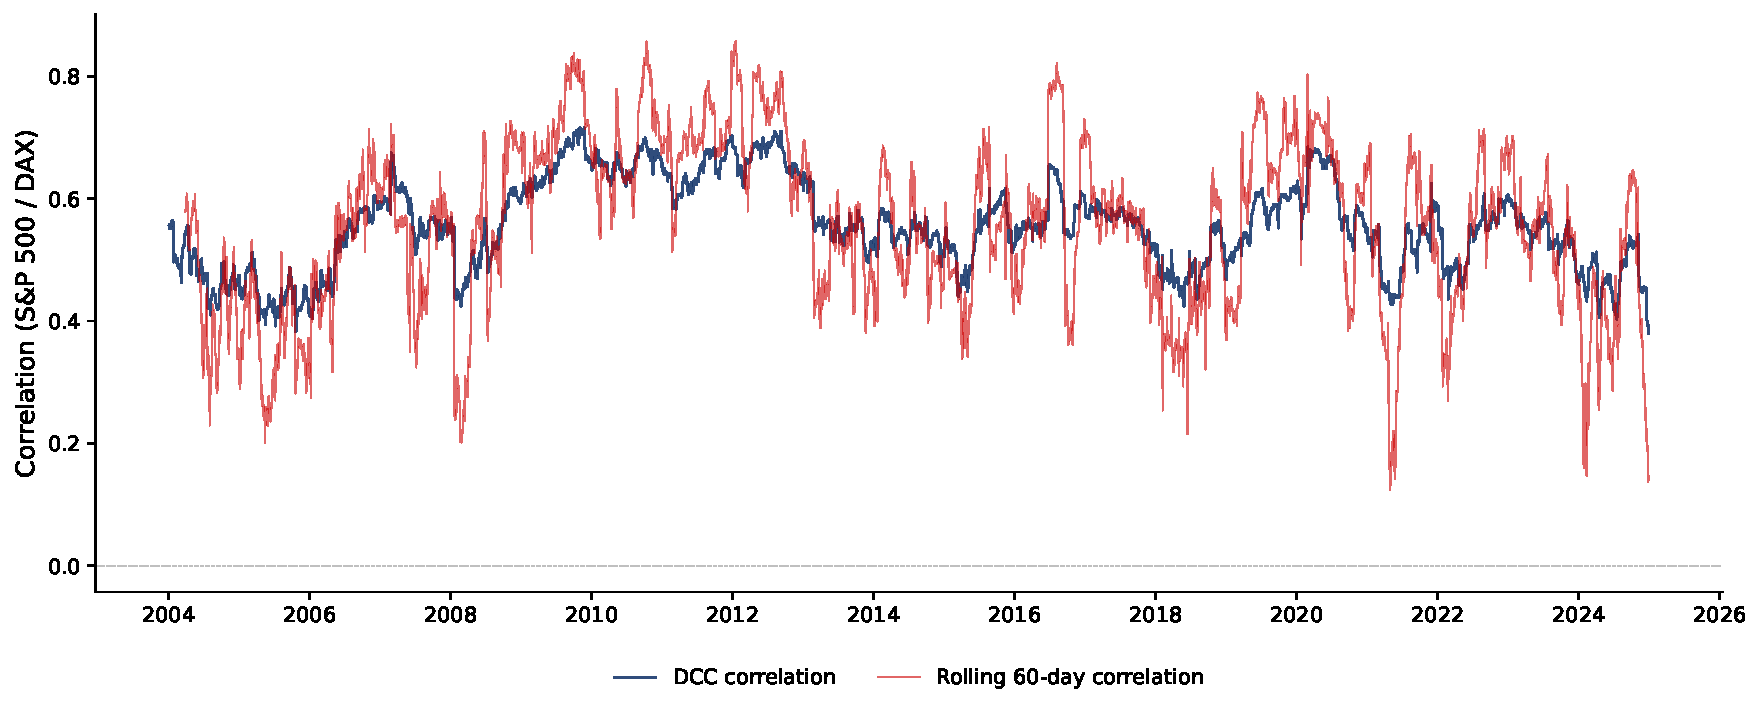
\includegraphics[width=0.95\textwidth, height=0.72\textheight, keepaspectratio]{../../charts/ch5b_dcc_vs_rolling.pdf}
        \end{center}
    \end{cminipage}
    \hfill\quantlet{TSA\_ch5b\_dcc\_estimation}{https://github.com/QuantLet/TSA/tree/main/TSA\_ch5b/TSA\_ch5b\_dcc\_estimation}
\end{frame}

\begin{frame}{News Impact on DCC Correlation}
    \begin{cminipage}{0.95\textwidth}
    \vspace{-2mm}
        \begin{center}
            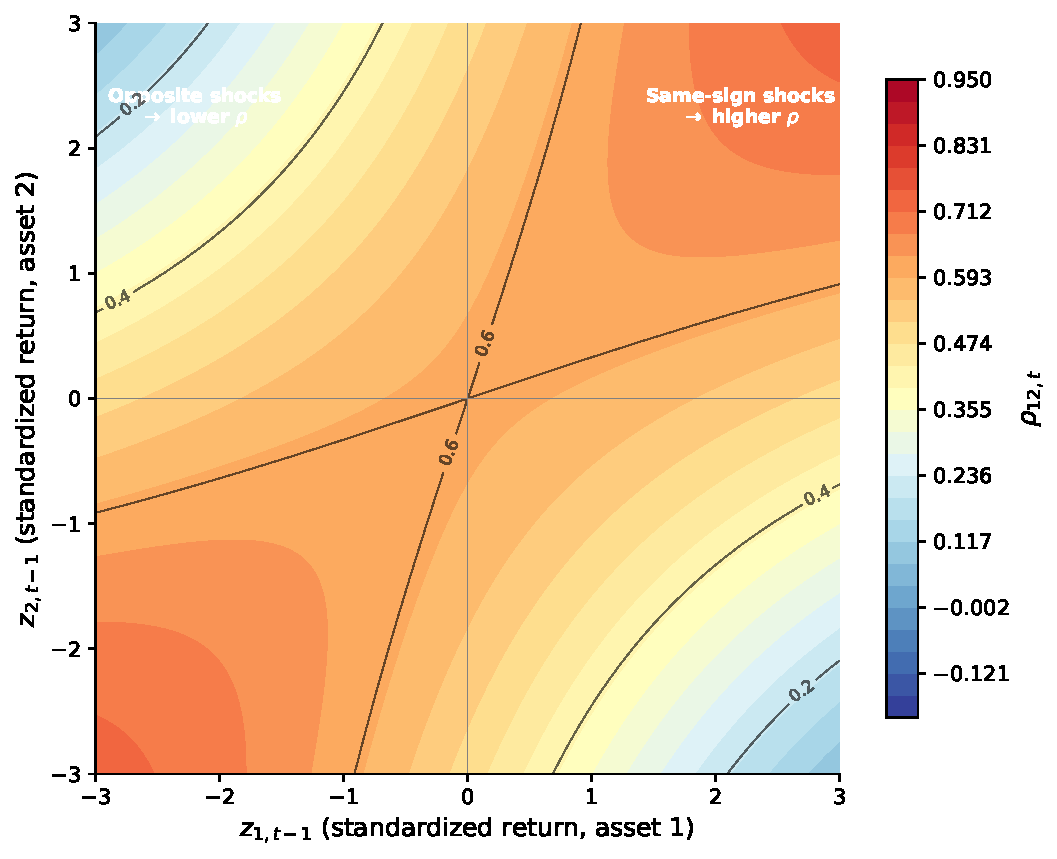
\includegraphics[width=0.85\textwidth, height=0.62\textheight, keepaspectratio]{../../charts/ch5b_news_impact_correlation.pdf}
        \end{center}
    \vspace{-2mm}
    {\footnotesize
    \begin{alertblock}{Interpretation}
        \begin{itemize}\setlength{\itemsep}{0pt}
            \item When both assets experience shocks of the \textbf{same sign}, correlation \textbf{increases}
            \item \textbf{Opposite-sign} shocks reduce correlation --- decoupling effect
        \end{itemize}
    \end{alertblock}
    }
    \end{cminipage}
    \hfill\quantlet{TSA\_ch5b\_news\_impact\_corr}{https://github.com/QuantLet/TSA/tree/main/TSA\_ch5b/TSA\_ch5b\_news\_impact\_corr}
\end{frame}

\begin{frame}{Covariance Decomposition: $\mathbf{H}_t = \mathbf{D}_t \mathbf{R}_t \mathbf{D}_t$}
    \begin{cminipage}{0.95\textwidth}
        \begin{center}
            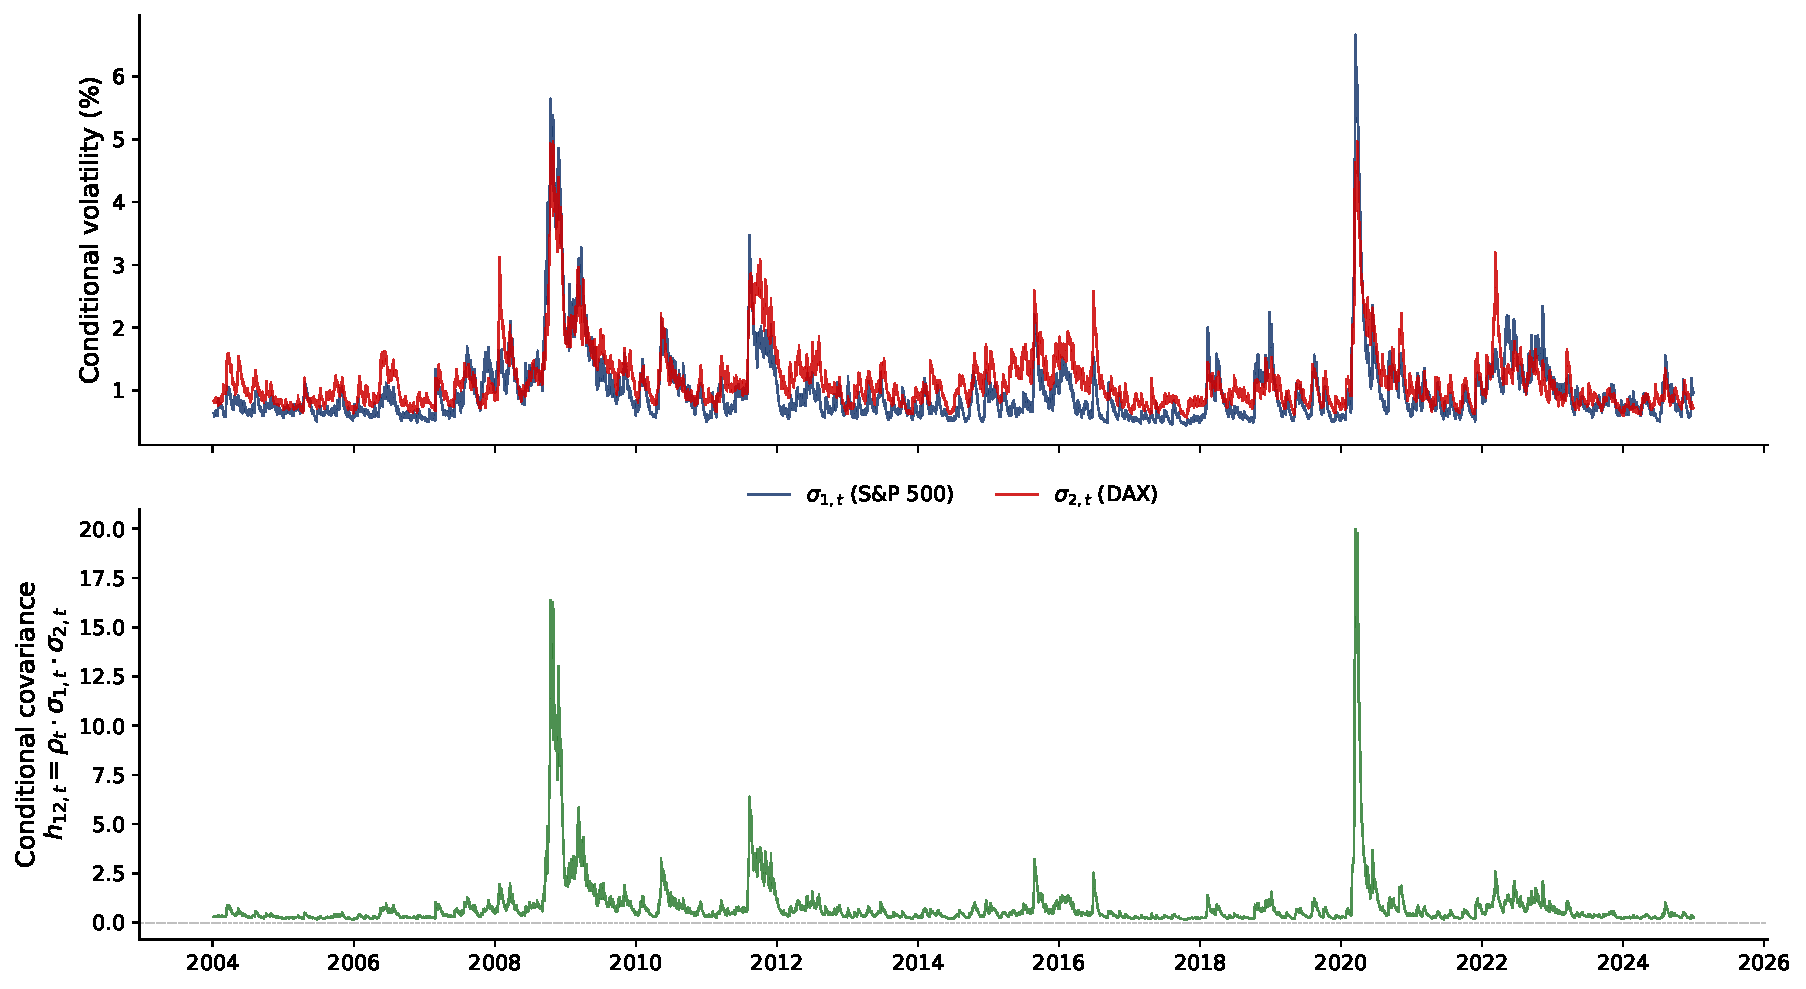
\includegraphics[width=0.95\textwidth, height=0.72\textheight, keepaspectratio]{../../charts/ch5b_covariance_decomp.pdf}
        \end{center}
    \end{cminipage}
    \hfill\quantlet{TSA\_ch5b\_cov\_decomp}{https://github.com/QuantLet/TSA/tree/main/TSA\_ch5b/TSA\_ch5b\_cov\_decomp}
\end{frame}

\begin{frame}{Numerical Example: DCC Step by Step}
    \begin{cminipage}{0.95\textwidth}
    \vspace{-4mm}
    {\scriptsize
    \begin{exampleblock}{Data: S\&P 500 and DAX, day $t-1$}
        \begin{itemize}\setlength{\itemsep}{0pt}
            \item Standardized residuals: $z_{1,t-1} = -2.1$ (S\&P 500), $z_{2,t-1} = -1.8$ (DAX)
            \item Parameters: $a = 0.05$, $b = 0.93$, $\bar{q}_{12} = 0.65$
            \item Previous state: $q_{11,t-1} = 1.02$, $q_{22,t-1} = 0.98$, $q_{12,t-1} = 0.68$
        \end{itemize}
    \end{exampleblock}
    \begin{block}{Step 1: Update $\mathbf{Q}_t$}
        \begin{align*}
            q_{11,t} &= (1 - 0.05 - 0.93) \cdot 1 + 0.05 \cdot (-2.1)^2 + 0.93 \cdot 1.02 = 0.02 + 0.2205 + 0.9486 = \textcolor{MainBlue}{1.189} \\
            q_{22,t} &= 0.02 + 0.05 \cdot (-1.8)^2 + 0.93 \cdot 0.98 = 0.02 + 0.162 + 0.9114 = \textcolor{MainBlue}{1.093} \\
            q_{12,t} &= 0.02 \cdot 0.65 + 0.05 \cdot (-2.1)(-1.8) + 0.93 \cdot 0.68 = 0.013 + 0.189 + 0.6324 = \textcolor{MainBlue}{0.834}
        \end{align*}
    \end{block}
    \begin{block}{Step 2: Rescale $\rightarrow$ correlation $\rho_{12,t}$}
        \vspace{-2mm}
        \[
            \rho_{12,t} = \frac{q_{12,t}}{\sqrt{q_{11,t} \cdot q_{22,t}}} = \frac{0.834}{\sqrt{1.189 \cdot 1.093}} = \frac{0.834}{1.140} = \textcolor{Crimson}{\mathbf{0.732}}
        \]
        \vspace{-3mm}
        \textit{Correlation rose from $\approx 0.67$ to $\textcolor{Crimson}{0.73}$ due to joint negative shocks!}
    \end{block}
    }
    \end{cminipage}
\end{frame}

\begin{frame}{DCC vs CCC: When Does It Matter?}
    \begin{cminipage}{0.95\textwidth}
    {\footnotesize
    \begin{block}{Testing for Constant Correlation}
        \begin{itemize}\setlength{\itemsep}{0pt}
            \item \textbf{Engle--Sheppard (2001) test}: $H_0$: correlations are constant
                \begin{itemize}\setlength{\itemsep}{0pt}
                    \item Regress $\text{vech}(\mathbf{z}_t\mathbf{z}_t' - \hat{\mathbf{R}})$ on lagged values
                    \item $T \cdot R^2 \sim \chi^2$ under $H_0$
                \end{itemize}
        \end{itemize}
    \end{block}
    \vspace{0.1cm}
    \begin{block}{Empirical Evidence}
        \begin{itemize}\setlength{\itemsep}{0pt}
            \item CCC is almost \textbf{always rejected} in financial data
            \item DCC provides better out-of-sample portfolio performance
            \item The improvement is largest during \textbf{crisis periods}
        \end{itemize}
    \end{block}
    \vspace{0.1cm}
    \begin{alertblock}{Practical Rule}
        \begin{itemize}\setlength{\itemsep}{0pt}
            \item Use CCC as a \textbf{benchmark} and DCC as the \textbf{workhorse} model. If the Engle--Sheppard test rejects CCC, use DCC.
        \end{itemize}
    \end{alertblock}
    }
    \end{cminipage}
\end{frame}

\begin{frame}{The Tse (2000) LM Test for Constant Correlation}
    \begin{cminipage}{0.95\textwidth}
    \vspace{-3mm}
    {\scriptsize
    \begin{block}{Hypotheses}
        \begin{itemize}\setlength{\itemsep}{0pt}
            \item $H_0$: $\rho_{ij,t} = \rho_{ij}$ $\forall t$ (correlations are \textbf{constant} --- CCC model is correct)
            \item $H_1$: $\rho_{ij,t}$ varies over time (a DCC model is needed)
        \end{itemize}
    \end{block}
    \vspace{-2mm}
    \begin{block}{Test Construction}
        \begin{itemize}\setlength{\itemsep}{0pt}
            \item Estimate CCC and obtain standardized residuals $\hat{z}_{it} = \hat{\varepsilon}_{it}/\hat{\sigma}_{it}$
            \item Compute pairwise products: $\hat{u}_{ij,t} = \hat{z}_{it}\hat{z}_{jt} - \hat{\rho}_{ij}$ for each pair $(i,j)$
            \item Regress $\hat{u}_{ij,t}$ on $p$ lagged values $\hat{u}_{ij,t-1}, \ldots, \hat{u}_{ij,t-p}$
            \item Test statistic: $LM = T \sum_{i<j} R^2_{ij} \xrightarrow{d} \chi^2\big(\frac{N(N-1)}{2} \cdot p\big)$ under $H_0$
        \end{itemize}
    \end{block}
    \vspace{-2mm}
    \begin{alertblock}{Difference from Engle--Sheppard (2001)}
        \begin{itemize}\setlength{\itemsep}{0pt}
            \item \textbf{Engle--Sheppard}: regresses the vector $\text{vech}(\mathbf{z}_t\mathbf{z}_t' - \hat{\mathbf{R}})$ \textbf{jointly} on lagged values --- tests all pairs in a single regression
            \item \textbf{Tse}: tests each pair $(i,j)$ \textbf{separately}, then combines the statistics --- easier to interpret but less powerful for complex dependencies
        \end{itemize}
    \end{alertblock}
    }
    \end{cminipage}
\end{frame}

%=============================================================================
% DCC: KEY INSIGHT + PITFALL
%=============================================================================

\begin{frame}{DCC: Key Insight and Common Pitfalls}
    \begin{cminipage}{0.95\textwidth}
    \vspace{-4mm}
    {\scriptsize
    \begin{block}{\textcolor{MainBlue}{$\blacktriangleright$ Key Insight}: DCC captures correlation dynamics with just 2 parameters}
        \begin{itemize}\setlength{\itemsep}{0pt}
            \item $a$ and $b$ are \textbf{shared across all pairs} --- for 100 assets, 4,950 correlations share 2 parameters
            \item This is simultaneously its greatest strength (scalability) and limitation (homogeneity)
        \end{itemize}
    \end{block}
    \vspace{-2mm}
    \begin{alertblock}{\textcolor{Crimson}{$\blacktriangleright$ Common Pitfalls}}
        \begin{itemize}\setlength{\itemsep}{0pt}
            \item \textbf{Ignoring Aielli (2013)}: original DCC is inconsistent ($E[\mathbf{Q}_t] \neq \bar{\mathbf{Q}}$). Use cDCC.
            \item \textbf{Same-speed assumption}: stock--bond fast, stock--stock slow --- single $(a,b)$ compromises
            \item \textbf{Forgetting sandwich}: naive SEs from two-step are \textbf{wrong} --- use Bollerslev--Wooldridge
        \end{itemize}
    \end{alertblock}
    \vspace{-2mm}
    \begin{exampleblock}{\textcolor{Forest}{$\blacktriangleright$ When NOT to use DCC}}
        \begin{itemize}\setlength{\itemsep}{0pt}
            \item Need \textbf{spillover direction}: use BEKK or Diebold--Yilmaz instead
            \item Correlations \textbf{genuinely constant}: DCC adds noise; CCC is more efficient
            \item Assets have very \textbf{different correlation dynamics}: consider block-DCC or copula
        \end{itemize}
    \end{exampleblock}
    }
    \end{cminipage}
\end{frame}

\begin{frame}{DCC Section Summary}
    \begin{cminipage}{0.95\textwidth}
    {\footnotesize
    \begin{block}{3 Things to Remember}
        \begin{enumerate}\setlength{\itemsep}{2pt}
            \item DCC = CCC with dynamic $\mathbf{R}_t$: only \textbf{2 extra parameters} ($a, b$) for all $N(N-1)/2$ correlations
            \item $\mathbf{Q}_t$ equation is a GARCH(1,1) for correlations: $a$ = shock reactivity, $b$ = persistence
            \item Two-step estimation is consistent but needs \textbf{sandwich standard errors}
        \end{enumerate}
    \end{block}
    \begin{alertblock}{Model Positioning}
        \begin{itemize}\setlength{\itemsep}{0pt}
            \item \textbf{Use as}: the \textbf{industry workhorse} --- best balance of flexibility and scalability
            \item \textbf{vs.\ CCC}: captures crisis correlation spikes \quad \textbf{vs.\ BEKK}: no spillover direction, but scales to $N > 100$
        \end{itemize}
    \end{alertblock}
    }
    \end{cminipage}
\end{frame}

%=============================================================================
% SECTION 7: OTHER MULTIVARIATE GARCH MODELS
%=============================================================================
\section{Other Multivariate GARCH Models}

\begin{frame}{Asymmetric DCC (aDCC) -- Cappiello, Engle \& Sheppard (2006)}
    \begin{cminipage}{0.95\textwidth}
    {\footnotesize
    \begin{block}{Motivation: Leverage in Correlations}
        \begin{itemize}\setlength{\itemsep}{0pt}
            \item Correlations may respond asymmetrically to negative vs.\ positive shocks (``correlation leverage''). The aDCC extends DCC:
        \end{itemize}
        \[
            \mathbf{Q}_t = (\bar{\mathbf{Q}} - a\bar{\mathbf{Q}} - b\bar{\mathbf{Q}} - g\bar{\mathbf{N}}) + a\,\mathbf{z}_{t-1}\mathbf{z}_{t-1}' + b\,\mathbf{Q}_{t-1} + g\,\underbrace{\mathbf{n}_{t-1}\mathbf{n}_{t-1}'}_{\text{asymmetric term}}
        \]
        \begin{itemize}\setlength{\itemsep}{0pt}
            \item where $\mathbf{n}_t = \mathbf{z}_t \odot \mathbf{1}(\mathbf{z}_t < 0)$ and $\bar{\mathbf{N}} = T^{-1}\sum_t \mathbf{n}_t\mathbf{n}_t'$
        \end{itemize}
        \textit{Intuition: joint losses ($g$ term) can increase correlations more than joint gains --- the ``bad news'' amplifier.}
    \end{block}
    \vspace{0.1cm}
    \begin{block}{Properties}
        \begin{itemize}\setlength{\itemsep}{0pt}
            \item Adds only \textbf{one parameter} ($g$) to the DCC model
            \item Captures the empirical finding that correlations increase more after \textbf{joint negative shocks}
            \item Nests DCC ($g=0$) and CCC ($a=b=g=0$) as special cases
        \end{itemize}
    \end{block}
    }
    \end{cminipage}
\end{frame}

\begin{frame}{GO-GARCH (van der Weide, 2002)}
    \begin{cminipage}{0.95\textwidth}
    {\footnotesize
    \begin{block}{Idea: Generalized Orthogonal GARCH}
        \begin{itemize}\setlength{\itemsep}{0pt}
            \item Map the $N$-dimensional return vector to $N$ \textbf{uncorrelated factors}:
        \end{itemize}
        \[
            \boldsymbol{\varepsilon}_t = \mathbf{Z}\mathbf{f}_t, \qquad \mathbf{f}_t = (f_{1t}, \ldots, f_{Nt})'
        \]
        \begin{itemize}\setlength{\itemsep}{0pt}
            \item where $\mathbf{Z}$ is a mixing matrix and the factors $f_{it}$ are \textbf{uncorrelated} with individual GARCH dynamics:
        \end{itemize}
        \[
            \sigma_{f_i,t}^2 = \omega_i + \alpha_i f_{i,t-1}^2 + \beta_i \sigma_{f_i,t-1}^2
        \]
    \end{block}
    \vspace{0.1cm}
    \begin{block}{Reconstruction}
        \[
            \mathbf{H}_t = \mathbf{Z}\,\text{diag}(\sigma_{f_1,t}^2, \ldots, \sigma_{f_N,t}^2)\,\mathbf{Z}'
        \]
        \textit{Intuition: model volatility in ``factor space'' (simple), then rotate back to ``asset space'' (complex).}
        \begin{itemize}\setlength{\itemsep}{0pt}
            \item Positive definite \textbf{by construction}
            \item Parameters: $N(N-1)/2 + 3N$ --- scales well with $N$
            \item Related to Independent Component Analysis (ICA)
        \end{itemize}
    \end{block}
    }
    \end{cminipage}
\end{frame}

\begin{frame}{Factor GARCH Models}
    \begin{cminipage}{0.95\textwidth}
    \vspace{-2mm}
    {\scriptsize
    \begin{block}{Idea: Reduce Dimensionality with Factors ($K \ll N$)}
        \vspace{-2mm}
        \[
            \boldsymbol{\varepsilon}_t = \mathbf{\Lambda}\mathbf{f}_t + \mathbf{u}_t
        \]
        \vspace{-3mm}
        \begin{itemize}\setlength{\itemsep}{0pt}
            \item $\mathbf{\Lambda}$: $N \times K$ loadings; $\mathbf{f}_t$: $K \times 1$ factors; $\mathbf{u}_t$: idiosyncratic
        \end{itemize}
        \vspace{-2mm}
        \[
            \mathbf{H}_t = \underbrace{\mathbf{\Lambda}\mathbf{H}_t^f\mathbf{\Lambda}'}_{\text{systematic risk}} + \underbrace{\boldsymbol{\Sigma}_t^u}_{\text{idiosyncratic risk}}
        \]
        \vspace{-2mm}
        \textit{Intuition: model a few common factors, treat the rest as noise.}
    \end{block}
    \begin{block}{Variants}
        \begin{itemize}\setlength{\itemsep}{0pt}
            \item \textbf{O-GARCH} (Alexander, 2001): PCA + diagonal GARCH on principal components
            \item \textbf{Factor GARCH} (Engle, Ng \& Rothschild, 1990): parametric factor structure
            \item \textbf{DCC-MIDAS} (Colacito, Engle \& Ghysels, 2011): mixed-frequency correlations
        \end{itemize}
    \end{block}
    \begin{alertblock}{When to Use}
        \begin{itemize}\setlength{\itemsep}{0pt}
            \item The \textbf{go-to approach} for large $N$ (50--500 assets): parsimony + economic interpretability.
        \end{itemize}
    \end{alertblock}
    }
    \end{cminipage}
\end{frame}

\begin{frame}{Tse--Tsui DCC (2002)}
    \begin{cminipage}{0.95\textwidth}
    {\footnotesize
    \begin{block}{An Alternative to Engle's DCC}
        \begin{itemize}\setlength{\itemsep}{0pt}
            \item Tse \& Tsui (2002) propose a different dynamics for $\mathbf{R}_t$:
            \[
                \mathbf{R}_t = (1 - \theta_1 - \theta_2)\underbrace{\mathbf{R}}_{\text{long-run}} + \theta_1 \underbrace{\boldsymbol{\Psi}_{t-1}}_{\text{local window}} + \theta_2 \underbrace{\mathbf{R}_{t-1}}_{\text{persistence}}
            \]
            \item \textit{Intuition: blend long-run, recent-window, and yesterday's correlation --- the result is automatically a valid correlation matrix.}
            \item $\boldsymbol{\Psi}_{t-1}$ = sample correlation over the last $M$ observations
        \end{itemize}
    \end{block}
    \begin{block}{Comparison with Engle's DCC}
        \begin{itemize}\setlength{\itemsep}{0pt}
            \item \textbf{Advantage}: $\mathbf{R}_t$ is a proper correlation matrix \textbf{by construction} (no rescaling needed)
            \item \textbf{Disadvantage}: requires choosing window $M$; less used in practice
            \item Both models yield similar empirical results
        \end{itemize}
    \end{block}
    }
    \end{cminipage}
\end{frame}

\begin{frame}{Copula-GARCH: A Flexible Approach}
    \begin{cminipage}{0.95\textwidth}
    \vspace{-3mm}
    {\scriptsize
    \begin{block}{Idea: Separate Margins from Dependence Structure}
        \begin{itemize}\setlength{\itemsep}{0pt}
            \item \textbf{Sklar's Theorem}: $F(x_1, \ldots, x_N) = C\big(F_1(x_1), \ldots, F_N(x_N)\big)$
            \item \textit{Intuition: model each asset's risk profile separately, then ``glue'' them together with a copula.}
            \item $F_i$ = marginal distributions (GARCH + flexible dist.); $C$ = copula (dependence structure)
        \end{itemize}
    \end{block}
    \vspace{-1mm}
    \begin{block}{Advantages over DCC}
        \begin{itemize}\setlength{\itemsep}{0pt}
            \item Allows \textbf{asymmetric tail dependence}; margins can have \textbf{different} distributions (Student-$t$, skewed-$t$, GED)
            \item $t$-Student copula: DCC-like $\rho_t$ + tail dependence parameterized by $\nu$
        \end{itemize}
    \end{block}
    \vspace{-1mm}
    \begin{alertblock}{Implementation}
        \begin{itemize}\setlength{\itemsep}{0pt}
            \item R: \texttt{copula} + \texttt{rugarch}; Python: \texttt{copulae}
        \end{itemize}
    \end{alertblock}
    }
    \end{cminipage}
\end{frame}

\begin{frame}{EWMA and RiskMetrics}
    \begin{cminipage}{0.95\textwidth}
    {\footnotesize
    \begin{block}{Exponentially Weighted Moving Average (EWMA)}
        \begin{itemize}\setlength{\itemsep}{0pt}
            \item The simplest multivariate volatility model --- no estimation needed:
        \end{itemize}
        \vspace{-2mm}
        \[
            \mathbf{H}_t = (1-\lambda)\boldsymbol{\varepsilon}_{t-1}\boldsymbol{\varepsilon}_{t-1}' + \lambda\mathbf{H}_{t-1}, \qquad \lambda = 0.94 \text{ (daily)}
        \]
        \vspace{-2mm}
        \textit{Intuition: weighted average of yesterday's forecast and realized shocks --- no estimation required.}
    \end{block}
    \begin{block}{Connection to MGARCH}
        \begin{itemize}\setlength{\itemsep}{0pt}
            \item EWMA $\equiv$ Scalar BEKK with $\omega = 0$, $a^2 = 1-\lambda$, $b^2 = \lambda$
            \item Also equivalent to IGARCH ($\alpha + \beta = 1$) without intercept
            \item RiskMetrics (J.P.\ Morgan, 1996) used this as the \textbf{industry standard}
        \end{itemize}
    \end{block}
    \vspace{0.1cm}
    \begin{alertblock}{Limitations}
        \begin{itemize}\setlength{\itemsep}{0pt}
            \item No estimation $\Rightarrow$ cannot adapt to different market conditions
            \item $\lambda = 0.94$ may not be optimal for all asset classes
            \item No asymmetric effects, no mean reversion in variance
        \end{itemize}
    \end{alertblock}
    }
    \end{cminipage}
\end{frame}

\begin{frame}{Model Taxonomy: A Summary}
    \begin{cminipage}{0.95\textwidth}
    {\scriptsize
    \begin{center}
    \begin{tabular}{lcccc}
        \hline
        \textbf{Model} & \textbf{P.D.} & \textbf{Spillovers} & \textbf{Dynamic $\rho$} & \textbf{Max $N$} \\
        \hline
        VEC & No$^*$ & Yes & Yes & $\sim 3$ \\
        Diagonal VEC & Yes$^*$ & No & Yes & $\sim 10$ \\
        BEKK (full) & Yes & Yes & Yes & $\sim 5$ \\
        Diagonal BEKK & Yes & No & Yes & $\sim 20$ \\
        Scalar BEKK / EWMA & Yes & No & Yes & $\sim 100$ \\
        CCC & Yes & No & No & $\sim 100$ \\
        DCC & Yes & No & Yes & $\sim 500$ \\
        aDCC & Yes & No & Yes & $\sim 500$ \\
        GO-GARCH & Yes & No & Yes & $\sim 50$ \\
        Factor GARCH & Yes & No & Yes & $\sim 500$ \\
        \hline
    \end{tabular}
    \end{center}
    \vspace{0.1cm}
    $^*$ Requires additional parameter restrictions.
    }
    \vspace{0.1cm}
    \begin{alertblock}{}
        {\footnotesize
        \begin{itemize}\setlength{\itemsep}{0pt}
            \item The choice of model depends on: (1) number of assets, (2) need for spillover effects, (3) need for dynamic correlations, (4) computational budget.
        \end{itemize}
        }
    \end{alertblock}
    \end{cminipage}
\end{frame}

\begin{frame}{Multivariate GARCH Model Hierarchy}
    \begin{cminipage}{0.95\textwidth}
    {\footnotesize
    \begin{block}{Nesting Relationships}
        \begin{itemize}\setlength{\itemsep}{0pt}
            \item EWMA $\subset$ Scalar BEKK $\subset$ Diagonal BEKK $\subset$ Full BEKK $\subset$ Full VEC
            \item CCC $\subset$ DCC $\subset$ aDCC
            \item DCC and Diagonal BEKK: \textbf{not} nested in each other
        \end{itemize}
    \end{block}
    \begin{block}{Choosing by Objective}
        \vspace{0.1cm}
        \begin{center}
        {\scriptsize
        \begin{tabular}{lll}
            \hline
            \textbf{Objective} & \textbf{Recommended Model} & \textbf{Why} \\
            \hline
            Portfolio VaR & DCC / aDCC & Dynamic correlations, scalable \\
            Optimal hedging & DCC / Diagonal BEKK & Time-varying covariance \\
            Shock transmission & Full BEKK & Captures spillovers \\
            $N > 100$ assets & Factor GARCH / DCC & Parsimony, feasibility \\
            Correlation asymmetry & aDCC & Leverage term $g$ \\
            Tail dependence & Copula-GARCH & Distributional flexibility \\
            \hline
        \end{tabular}
        }
        \end{center}
    \end{block}
    }
    \end{cminipage}
\end{frame}

%=============================================================================
% SECTION 8: LIMITATIONS OF MGARCH
%=============================================================================
\section{Limitations of MGARCH Models}

\begin{frame}{When MGARCH Models Fail}
    \begin{cminipage}{0.95\textwidth}
    \vspace{-4mm}
    {\scriptsize
    \begin{block}{Model Misspecification}
        \begin{itemize}\setlength{\itemsep}{0pt}
            \item All MGARCH assume a \textbf{parametric structure} for $\mathbf{H}_t$ --- the true DGP may not belong to this class
            \item DCC: \textbf{one correlation dynamic for all pairs} ($a$, $b$ scalars), yet equity-bond and equity-equity behave differently
            \item BEKK: \textbf{quadratic} dynamics --- cannot capture regime switches or structural breaks
            \item Gaussian QML: \textbf{consistent but inefficient} under fat tails --- losses grow with $N$
        \end{itemize}
    \end{block}
    \vspace{-3mm}
    \begin{block}{Tail Risk Failures}
        \begin{itemize}\setlength{\itemsep}{0pt}
            \item Normal innovations \textbf{underestimate joint tail risk}: $\Pr(\text{all assets crash})$ too low
            \item Student-$t$ copula: \textbf{symmetric} tail dependence --- assets crash together but don't boom together
            \item VaR violations in crises are \textbf{clustered} --- even DCC with correct coverage has concentrated violations
        \end{itemize}
    \end{block}
    \vspace{-3mm}
    \begin{alertblock}{Key Insight}
        \begin{itemize}\setlength{\itemsep}{0pt}
            \item MGARCH: \textbf{local approximations} --- work well in stable regimes, underperform during regime transitions
        \end{itemize}
    \end{alertblock}
    }
    \end{cminipage}
\end{frame}

\begin{frame}{Crisis Instability and the DCC Paradox}
    \begin{cminipage}{0.95\textwidth}
    \vspace{-3mm}
    {\scriptsize
    \begin{block}{The DCC Paradox}
        \begin{itemize}\setlength{\itemsep}{0pt}
            \item DCC is \textbf{most needed} during crises --- but crises are precisely when it is \textbf{least reliable}
            \item Parameter estimates from tranquil periods may \textbf{not apply} to crisis dynamics
            \item Aielli (2013): standard DCC estimator has \textbf{bias} in two-step procedure --- cDCC corrects this
        \end{itemize}
    \end{block}
    \vspace{-2mm}
    \begin{block}{Structural Breaks in Correlations}
        \begin{itemize}\setlength{\itemsep}{0pt}
            \item \textbf{Euro (1999)}: European equity correlations shifted permanently upward
            \item \textbf{GFC (2008)}: cross-asset correlations jumped and did not fully revert for years
            \item \textbf{COVID (2020)}: unprecedented correlation spike followed by rapid decorrelation
            \item DCC mean-reversion ($a + b < 1$) forces correlations to $\bar{Q}$ --- can be \textbf{wrong} after structural breaks
        \end{itemize}
    \end{block}
    \vspace{-2mm}
    \begin{alertblock}{Remedies}
        \begin{itemize}\setlength{\itemsep}{0pt}
            \item \textbf{DCC-MIDAS} (Colacito, Engle \& Ghysels, 2011): separates short-run and long-run correlation
            \item \textbf{Markov-Switching DCC}: discrete regime changes in correlation dynamics
            \item \textbf{Rolling windows}: re-estimate every 1--2 years to capture structural shifts
        \end{itemize}
    \end{alertblock}
    }
    \end{cminipage}
\end{frame}

\begin{frame}{Overfitting vs.\ Parsimony: The Bias-Variance Trade-off}
    \begin{cminipage}{0.95\textwidth}
    \vspace{-2mm}
    {\scriptsize
    \begin{block}{The Overfitting Trap}
        \begin{itemize}\setlength{\itemsep}{0pt}
            \item Full BEKK for $N = 5$: \textbf{55 parameters} --- fits in-sample perfectly, poor out-of-sample
            \item aDCC asymmetry ($+1$ parameter) helps for equities but may overfit bond-commodity pairs
            \item Student-$t$ d.f.\ $\nu$ can \textbf{compensate} for correlation misspecification, masking the real problem
        \end{itemize}
    \end{block}
    \vspace{-1mm}
    \begin{block}{Empirical Evidence (Caporin \& McAleer, 2012; Laurent et al., 2012)}
        \begin{itemize}\setlength{\itemsep}{0pt}
            \item \textbf{Scalar BEKK $\approx$ DCC} in out-of-sample forecasting for most portfolios
            \item Adding complexity beyond DCC(1,1) rarely improves portfolio VaR or hedging effectiveness
            \item The \textbf{simple EWMA ($\lambda = 0.94$)} remains a competitive benchmark --- hard to beat consistently
            \item Information criteria (AIC/BIC) favor DCC over BEKK for $N > 3$
        \end{itemize}
    \end{block}
    \begin{alertblock}{Practical Rule}
        \begin{itemize}\setlength{\itemsep}{0pt}
            \item Start simple (EWMA or CCC), add complexity \textbf{only if out-of-sample tests justify it}
            \item Use \textbf{Model Confidence Sets} (Hansen, Lunde \& Nason, 2011) rather than single-model selection
        \end{itemize}
    \end{alertblock}
    }
    \end{cminipage}
\end{frame}

\begin{frame}{Empirical Model Comparison: What the Literature Shows}
    \begin{cminipage}{0.95\textwidth}
    \vspace{-3mm}
    {\scriptsize
    \begin{block}{Out-of-Sample Forecasting Performance (Based on Laurent et al., 2012; Caporin \& McAleer, 2014)}
        \vspace{-1mm}
        \begin{center}
        \begin{tabular}{lccccc}
            \hline
            \textbf{Model} & \textbf{Portfolio VaR} & \textbf{Hedge} & \textbf{GMVP} & \textbf{Speed} & \textbf{Max $N$} \\
            \hline
            EWMA ($\lambda\!=\!0.94$) & Good & Fair & Fair & $\star\star\star\star\star$ & 1000+ \\
            CCC-GARCH & Fair & Fair & Poor & $\star\star\star\star$ & 500 \\
            DCC-GARCH & \textbf{Good} & \textbf{Good} & Good & $\star\star\star\star$ & 500 \\
            aDCC-GARCH & \textbf{Good} & \textbf{Good} & \textbf{Good} & $\star\star\star$ & 300 \\
            Diagonal BEKK & Good & Good & Good & $\star\star\star$ & 20 \\
            Full BEKK & Fair$^*$ & Good & Fair$^*$ & $\star$ & 5 \\
            GO-GARCH & Good & Fair & Good & $\star\star$ & 50 \\
            Copula-DCC & \textbf{Best} & Good & Good & $\star\star$ & 100 \\
            \hline
        \end{tabular}
        \end{center}
        \vspace{-2mm}
        \begin{itemize}\setlength{\itemsep}{0pt}
            \item $^*$Full BEKK overfits in-sample, degrades out-of-sample for $N > 3$. GMVP = Global Minimum Variance Portfolio.
        \end{itemize}
    \end{block}
    \vspace{-2mm}
    \begin{alertblock}{Key Findings}
        \begin{itemize}\setlength{\itemsep}{0pt}
            \item DCC is the \textbf{best risk-adjusted choice} across most applications
            \item Copula-DCC dominates for \textbf{tail risk} (ES, extreme VaR) but at higher computational cost
            \item Complexity beyond aDCC yields \textbf{diminishing returns} for most portfolios
        \end{itemize}
    \end{alertblock}
    }
    \end{cminipage}
\end{frame}

%=============================================================================
% SECTION 9: ESTIMATION AND DIAGNOSTICS
%=============================================================================
\section{Estimation and Diagnostics}

\begin{frame}{Estimation Methods}
    \begin{cminipage}{0.95\textwidth}
    \vspace{-3mm}
    {\footnotesize
    \begin{block}{Maximum Likelihood Estimation (MLE)}
        \begin{itemize}\setlength{\itemsep}{0pt}
            \item \textbf{Full MLE}: jointly estimate all parameters --- optimal but computationally expensive
            \item \textbf{Two-step (Composite) MLE}: estimate univariate models first, then correlation parameters
                \begin{itemize}\setlength{\itemsep}{0pt}
                    \item Used by CCC, DCC, aDCC
                    \item Consistent but less efficient than full MLE
                \end{itemize}
        \end{itemize}
    \end{block}
    \begin{block}{Quasi-Maximum Likelihood (QML)}
        \begin{itemize}\setlength{\itemsep}{0pt}
            \item Use the Gaussian likelihood even if the true distribution is non-Gaussian
            \item QML estimator is \textbf{consistent} under mild regularity conditions
            \item Use \textbf{robust (sandwich) standard errors}: $\hat{V} = \hat{J}^{-1}\hat{I}\hat{J}^{-1}$
        \end{itemize}
    \end{block}
    \begin{block}{Alternative: Multivariate Student-$t$}
        \begin{itemize}\setlength{\itemsep}{0pt}
            \item Better captures fat tails: $\mathbf{z}_t \sim t_\nu(\mathbf{0}, \mathbf{I}_N)$
            \item Adds one parameter ($\nu$) for degrees of freedom
        \end{itemize}
    \end{block}
    }
    \end{cminipage}
\end{frame}

\begin{frame}{The Sandwich Estimator}
    \begin{cminipage}{0.95\textwidth}
    \vspace{-3mm}
    {\scriptsize
    \begin{block}{Why Is It Needed?}
        \begin{itemize}\setlength{\itemsep}{0pt}
            \item QML assumes Gaussian distribution, but financial data exhibit \textbf{fat tails} and \textbf{asymmetry}
            \item Parameters are \textbf{consistent}, but classical standard errors are \textbf{incorrect}
            \item Solution: the \textbf{sandwich} estimator of Bollerslev--Wooldridge (1992) corrects the standard errors
        \end{itemize}
    \end{block}
    \vspace{-2mm}
    \begin{block}{The ``Sandwich'' Structure --- Where the Name Comes From}
        \begin{itemize}\setlength{\itemsep}{0pt}
            \item Variance-covariance matrix of the estimator: $\hat{V}(\hat{\boldsymbol{\theta}}) = \underbrace{\hat{\mathbf{J}}^{-1}}_{\text{``bread''}} \underbrace{\hat{\mathbf{I}}}_{\text{``filling''}} \underbrace{\hat{\mathbf{J}}^{-1}}_{\text{``bread''}}$
            \item $\hat{\mathbf{J}} = -\frac{1}{T}\sum_t \frac{\partial^2 \ell_t}{\partial \boldsymbol{\theta}\partial \boldsymbol{\theta}'}$ \quad (the Hessian --- assumes the model is correct)
            \item $\hat{\mathbf{I}} = \frac{1}{T}\sum_t \frac{\partial \ell_t}{\partial \boldsymbol{\theta}} \frac{\partial \ell_t}{\partial \boldsymbol{\theta}'}$ \quad (outer product of gradients --- \textit{empirical}, no assumptions)
            \item \textit{Intuition: $\hat{\mathbf{J}}$ trusts the model; $\hat{\mathbf{I}}$ trusts the data. If correctly specified, $\mathbf{I} = \mathbf{J}$ and $\hat{V} = \mathbf{J}^{-1}$.}
        \end{itemize}
    \end{block}
    \vspace{-2mm}
    \begin{alertblock}{When to Use}
        \begin{itemize}\setlength{\itemsep}{0pt}
            \item \textbf{Always} under QML estimation (GARCH with Gaussian likelihood on non-Gaussian data)
            \item In two-step DCC estimation: stage 2 standard errors must be corrected for stage 1 uncertainty
        \end{itemize}
    \end{alertblock}
    }
    \end{cminipage}
\end{frame}

\begin{frame}{Diagnostic Checks}
    \begin{cminipage}{0.95\textwidth}
    {\footnotesize
    \begin{block}{Residual Diagnostics}
        \begin{itemize}\setlength{\itemsep}{0pt}
            \item After estimation, compute standardized residuals $\hat{\mathbf{z}}_t = \hat{\mathbf{D}}_t^{-1}\hat{\boldsymbol{\varepsilon}}_t$ and check:
        \end{itemize}
        \begin{enumerate}\setlength{\itemsep}{0pt}
            \item \textbf{No serial correlation} in $\hat{z}_{it}$ and $\hat{z}_{it}^2$ (Ljung--Box test for each series)
            \item \textbf{No cross-correlation} in $\hat{z}_{it}\hat{z}_{jt}$ (Hosking, 1980; Li \& McLeod, 1981)
            \item \textbf{Normality} of $\hat{\mathbf{z}}_t$ (if Gaussian likelihood assumed)
        \end{enumerate}
    \end{block}
    \vspace{0.1cm}
    \begin{block}{Model Comparison}
        \begin{itemize}\setlength{\itemsep}{0pt}
            \item \textbf{Information criteria}: AIC, BIC (\textit{Akaike/Bayesian Information Criterion}) (penalize over-parameterization)
            \item \textbf{Likelihood ratio tests}: nested models (CCC vs DCC)
            \item \textbf{Out-of-sample evaluation}: portfolio performance, VaR backtesting
            \item \textbf{Mincer--Zarnowitz regression}: forecast $\hat{h}_{ij,t}$ vs realized covariance
        \end{itemize}
    \end{block}
    }
    \end{cminipage}
\end{frame}

\begin{frame}{Practical Estimation: Tips and Pitfalls}
    \begin{cminipage}{0.95\textwidth}
    {\footnotesize
    \begin{block}{Practical Tips}
        \begin{itemize}\setlength{\itemsep}{0pt}
            \item \textbf{Starting values}: initialize from OLS (\textit{Ordinary Least Squares}) estimates or EWMA ($\lambda = 0.94$)
            \item \textbf{Returns}: use log-returns $\times 100$ (in percent) --- stabilizes optimization
            \item \textbf{Missing data}: align series on common dates; do not interpolate
            \item \textbf{Convergence}: run optimization from multiple starting points
        \end{itemize}
    \end{block}
    \begin{alertblock}{Common Pitfalls}
        \begin{itemize}\setlength{\itemsep}{0pt}
            \item \textbf{Nonsynchronous trading}: DAX closes at 17:30 CET, NYSE at 16:00 EST --- intraday correlations are underestimated
                \begin{itemize}\setlength{\itemsep}{0pt}
                    \item Solution: Scholes--Williams (1977) correction or open-to-open returns
                \end{itemize}
            \item \textbf{Structural breaks}: crises permanently alter correlation regimes --- DCC assumes a single regime
            \item \textbf{Student-$t$ overfitting}: degrees of freedom $\nu$ may compensate for other specification issues
        \end{itemize}
    \end{alertblock}
    }
    \end{cminipage}
\end{frame}

\begin{frame}{Model Selection: Practical Guidelines}
    \begin{cminipage}{0.95\textwidth}
    {\footnotesize
    \begin{block}{Decision Flowchart}
        \begin{enumerate}\setlength{\itemsep}{2pt}
            \item \textbf{How many assets?}
                \begin{itemize}\setlength{\itemsep}{0pt}
                    \item $N \leq 5$: BEKK, DCC, or aDCC
                    \item $5 < N \leq 50$: DCC, aDCC, GO-GARCH
                    \item $N > 50$: Factor GARCH, DCC-MIDAS, EWMA
                \end{itemize}
            \item \textbf{Do you need volatility spillovers?}
                \begin{itemize}\setlength{\itemsep}{0pt}
                    \item Yes: Full BEKK (small $N$) or Factor models
                    \item No: DCC family
                \end{itemize}
            \item \textbf{Is there asymmetry in correlations?}
                \begin{itemize}\setlength{\itemsep}{0pt}
                    \item Test for it $\Rightarrow$ if yes, use aDCC
                \end{itemize}
            \item \textbf{Validate}: check residual diagnostics, out-of-sample performance
        \end{enumerate}
    \end{block}
    }
    \end{cminipage}
\end{frame}

%=============================================================================
% SECTION 9: CASE STUDIES
%=============================================================================
\section{Case Studies}

%--- Case Study 1: Volatility Spillovers ---
\begin{frame}{Case Study 1: Volatility Spillovers Across Markets}
    \vspace{-2mm}
    {\scriptsize\textit{Learning goal: how BEKK off-diagonals reveal the direction of shock transmission between markets.}}\vspace{1mm}
    \begin{cminipage}{0.95\textwidth}
    {\scriptsize
    \begin{block}{Spillover Indicators}
        \begin{itemize}\setlength{\itemsep}{0pt}
            \item From the BEKK model: $\mathbf{H}_t = \mathbf{C}'\mathbf{C} + \mathbf{A}'\boldsymbol{\varepsilon}_{t-1}\boldsymbol{\varepsilon}_{t-1}'\mathbf{A} + \mathbf{B}'\mathbf{H}_{t-1}\mathbf{B}$
            \item \textbf{Spillover intensity} from asset $j$ to asset $i$:
            \[
                \text{Spillover}_{j \rightarrow i} = a_{ij}^2 + b_{ij}^2
            \]
            \item \textbf{Diebold--Yilmaz} index (2012): $S^H = \frac{1}{N}\sum_{i \neq j} \theta_{ij}^H$ where $\theta_{ij}^H$ = share of $i$'s variance due to shock $j$
        \end{itemize}
    \end{block}
    \begin{alertblock}{Methodology}
        \begin{itemize}\setlength{\itemsep}{0pt}
            \item Data: daily returns S\&P 500, DAX, FTSE 100, Nikkei 225 (2004--2024, $T \approx 5000$)
            \item Bivariate BEKK(1,1) for each pair of assets
        \end{itemize}
    \end{alertblock}
    }
    \end{cminipage}
\end{frame}

\begin{frame}{Case Study 1: What is a Volatility Spillover?}
    \begin{cminipage}{0.95\textwidth}
    {\footnotesize
    \begin{block}{Definition}
        \begin{itemize}\setlength{\itemsep}{0pt}
            \item A \textbf{volatility spillover} occurs when a shock in market $j$ increases the conditional variance of market $i$, beyond what $i$'s own past shocks and variances predict
        \end{itemize}
    \end{block}
    \vspace{-2mm}
    \begin{block}{Transmission Channels}
        \begin{itemize}\setlength{\itemsep}{0pt}
            \item \textbf{Direct financial linkages}: cross-border holdings, interbank lending, common counterparties
            \item \textbf{Information channel}: price discovery flows from developed to emerging markets
            \item \textbf{Behavioral channel}: herding, flight to quality, correlated margin calls
            \item \textbf{Time-zone effect}: NY close $\rightarrow$ Asian open $\rightarrow$ European open --- sequential transmission
        \end{itemize}
    \end{block}
    \vspace{-2mm}
    \begin{alertblock}{Why It Matters for Risk Management}
        \begin{itemize}\setlength{\itemsep}{0pt}
            \item Portfolio VaR depends on \textbf{cross-market} covariance, not just individual volatilities
            \item During crises, all channels activate simultaneously $\Rightarrow$ correlation spike $\Rightarrow$ diversification fails
            \item Example: Lehman collapse (Sep 2008) $\rightarrow$ US vol triples $\rightarrow$ DAX opens 5\% lower next day
        \end{itemize}
    \end{alertblock}
    }
    \end{cminipage}
\end{frame}

\begin{frame}{Case Study 1: BEKK Parameter Matrix --- Reading Off-Diagonals}
    \begin{cminipage}{0.95\textwidth}
    {\footnotesize
    \begin{block}{The $2 \times 2$ BEKK Structure (bivariate case)}
        \[
            \mathbf{A} = \begin{pmatrix} a_{11} & a_{12} \\ a_{21} & a_{22} \end{pmatrix}, \qquad
            \mathbf{B} = \begin{pmatrix} b_{11} & b_{12} \\ b_{21} & b_{22} \end{pmatrix}
        \]
        \begin{itemize}\setlength{\itemsep}{1pt}
            \item $a_{12}$: shock in asset 2 $\Rightarrow$ \textbf{immediate} volatility increase in asset 1
            \item $b_{12}$: conditional variance of asset 2 $\Rightarrow$ \textbf{persistent} effect on variance of asset 1
            \item Total spillover: $\text{Spillover}_{2 \rightarrow 1} = a_{12}^2 + b_{12}^2$
        \end{itemize}
    \end{block}
    \begin{exampleblock}{Numerical Example: S\&P 500 $\leftrightarrow$ DAX}
        {\small
        \begin{center}
        \begin{tabular}{l|cc|cc}
            \hline
            & $a_{12}$ & $a_{21}$ & $b_{12}$ & $b_{21}$ \\
            \hline
            Estimate & 0.18 & 0.09 & 0.31 & 0.15 \\
            Squared  & 0.032 & 0.008 & 0.096 & 0.023 \\
            \hline
        \end{tabular}
        \end{center}
        }
        \begin{itemize}\setlength{\itemsep}{0pt}
            \item Spillover$_{\text{SP}\rightarrow\text{DAX}} = 0.008 + 0.023 = 0.031$ \quad vs.\ Spillover$_{\text{DAX}\rightarrow\text{SP}} = 0.032 + 0.096 = 0.128$
            \item $\Rightarrow$ S\&P $\rightarrow$ DAX is \textbf{4$\times$ stronger} than DAX $\rightarrow$ S\&P
        \end{itemize}
    \end{exampleblock}
    }
    \end{cminipage}
\end{frame}

\begin{frame}{Case Study 1: Volatility Spillover Heatmap}
    \begin{cminipage}{0.95\textwidth}
    \vspace{-3mm}
        \begin{center}
            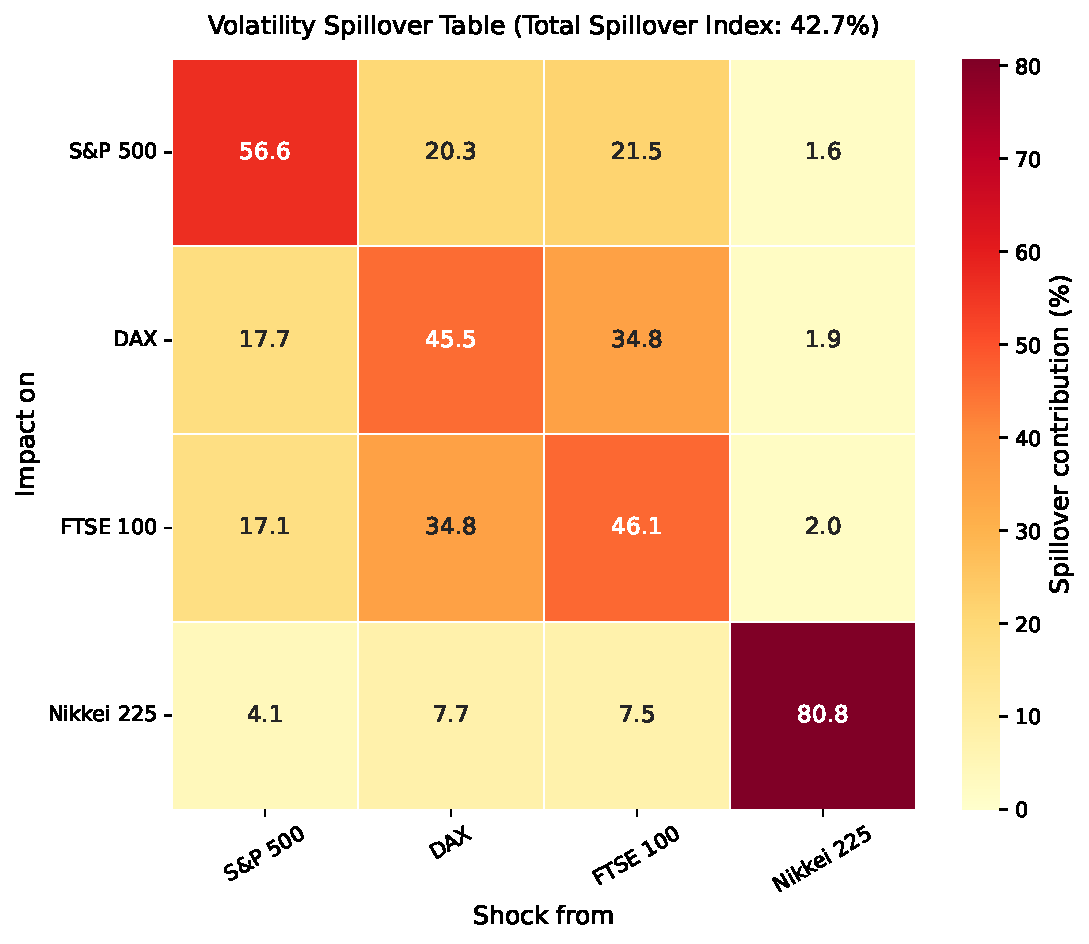
\includegraphics[width=0.82\textwidth, height=0.50\textheight, keepaspectratio]{../../charts/ch5b_spillover_heatmap.pdf}
        \end{center}
    \vspace{-3mm}
    {\scriptsize
    \begin{alertblock}{Key Results}
        \begin{itemize}\setlength{\itemsep}{0pt}
            \item S\&P 500 is the main volatility \textbf{exporter} --- US shocks propagate globally within 24h
            \item European markets (DAX, FTSE) are strongly \textbf{interconnected} (high reciprocal spillover)
            \item Nikkei is most \textbf{independent} --- time zone lag reduces direct transmission
            \item \textbf{Implication}: a global portfolio cannot ignore the US $\rightarrow$ Europe channel
        \end{itemize}
    \end{alertblock}
    }
    \end{cminipage}
    \hfill\quantlet{TSA\_ch5b\_spillover\_heatmap}{https://github.com/QuantLet/TSA/tree/main/TSA\_ch5b/TSA\_ch5b\_spillover\_heatmap}
\end{frame}

\begin{frame}{Case Study 1: Directed Spillovers --- Who Exports, Who Imports?}
    \begin{cminipage}{0.95\textwidth}
    {\footnotesize
    \begin{block}{Net Spillover = Transmitted $-$ Received}
        \vspace{0.1cm}
        {\small
        \begin{center}
        \begin{tabular}{l|ccc|c}
            \hline
            \textbf{Market} & \textbf{Transmitted} & \textbf{Received} & \textbf{Net} & \textbf{Role} \\
            \hline
            S\&P 500  & 66 & 55 & \textcolor{Crimson}{$+$11} & Net exporter \\
            DAX       & 61 & 62 & \textcolor{MainBlue}{$-$1} & Balanced \\
            FTSE 100  & 58 & 60 & \textcolor{MainBlue}{$-$2} & Slight importer \\
            Nikkei    & 32 & 40 & \textcolor{MainBlue}{$-$8} & Net importer \\
            \hline
        \end{tabular}
        \end{center}
        }
    \end{block}
    \begin{alertblock}{Interpretation}
        \begin{itemize}\setlength{\itemsep}{0pt}
            \item S\&P 500 is the \textbf{volatility hub}: it transmits more to every other market than it receives
            \item DAX and FTSE are nearly \textbf{balanced} --- they are both recipients of US shocks and transmitters to each other
            \item Nikkei is most \textbf{isolated}: receives 8 p.p.\ more than it sends --- time-zone lag acts as a natural barrier
            \item \textbf{Practical}: hedging US equity exposure is the single most impactful risk reduction action for a global portfolio
        \end{itemize}
    \end{alertblock}
    }
    \end{cminipage}
\end{frame}

\begin{frame}{Case Study 1: Diebold--Yilmaz Spillover Table}
    \begin{cminipage}{0.95\textwidth}
    \vspace{-2mm}
    {\footnotesize
    \begin{block}{VAR(5) on realized volatilities; horizon $H = 10$ days}
        \vspace{0.1cm}
        {\small
        \begin{center}
        \begin{tabular}{l|cccc|c}
            \hline
            \textbf{From $\rightarrow$} & S\&P & DAX & FTSE & Nikkei & \textbf{Received} \\
            \hline
            S\&P 500  & 45 & 22 & 20 & 13 & 55 \\
            DAX       & 25 & 38 & 28 &  9 & 62 \\
            FTSE 100  & 23 & 27 & 40 & 10 & 60 \\
            Nikkei    & 18 & 12 & 10 & 60 & 40 \\
            \hline
            \textbf{Transmitted} & 66 & 61 & 58 & 32 & $S^H \approx 54\%$ \\
            \hline
        \end{tabular}
        \end{center}
        }
    \end{block}
    \begin{alertblock}{Interpretation}
        \begin{itemize}\setlength{\itemsep}{0pt}
            \item S\&P 500: largest net \textbf{exporter} ($\text{transmitted} - \text{received} = 66 - 55 = +11$ p.p.)
            \item DAX and FTSE: strong bilateral spillover (28\%/27\%) --- tightly linked European markets
            \item Nikkei: most \textbf{isolated} ($32 - 40 = -8$ p.p.) --- receives more than it transmits
            \item $S^H \approx 54\%$: over half of volatility variation is due to cross-market \textbf{contagion}
        \end{itemize}
    \end{alertblock}
    }
    \end{cminipage}
    \hfill\quantlet{TSA\_ch5b\_spillover\_heatmap}{https://github.com/QuantLet/TSA/tree/main/TSA\_ch5b/TSA\_ch5b\_spillover\_heatmap}
\end{frame}

\begin{frame}{Case Study 1: Spillover Dynamics --- Calm vs.\ Crisis}
    \begin{cminipage}{0.95\textwidth}
    {\footnotesize
    \begin{block}{Rolling Diebold--Yilmaz Index ($H=10$, 252-day window)}
        \vspace{0.1cm}
        {\small
        \begin{center}
        \begin{tabular}{l|c|c|l}
            \hline
            \textbf{Period} & $S^H$ & \textbf{Top channel} & \textbf{Event} \\
            \hline
            2004--2006 & 42\% & SP $\rightarrow$ DAX & Pre-crisis calm \\
            2008--2009 & 72\% & SP $\rightarrow$ all & Global Financial Crisis \\
            2011--2012 & 65\% & DAX $\rightarrow$ FTSE & European sovereign debt \\
            2014--2019 & 48\% & SP $\rightarrow$ DAX & Post-crisis recovery \\
            2020 (Mar) & 70\% & SP $\rightarrow$ all & COVID-19 crash \\
            2022 & 58\% & SP $\rightarrow$ DAX & Monetary tightening \\
            \hline
        \end{tabular}
        \end{center}
        }
    \end{block}
    \begin{alertblock}{Key Insight}
        \begin{itemize}\setlength{\itemsep}{0pt}
            \item Spillover index nearly \textbf{doubles} during crises ($42\% \rightarrow 72\%$) --- diversification collapses exactly when it is needed most
            \item The US market dominates spillover in \textbf{all} crisis episodes --- no regime where Europe leads
            \item Recovery is asymmetric: post-GFC $S^H$ took 3 years to normalize; post-COVID only 6 months
        \end{itemize}
    \end{alertblock}
    }
    \end{cminipage}
\end{frame}

\begin{frame}{Case Study 1: Contagion Mechanisms During Crises}
    \begin{cminipage}{0.95\textwidth}
    {\footnotesize
    \begin{block}{Why Does Spillover Increase in Crises?}
        \begin{itemize}\setlength{\itemsep}{1pt}
            \item \textbf{Margin calls}: forced selling in one market $\Rightarrow$ deleveraging across all markets simultaneously
            \item \textbf{Liquidity spirals} (Brunnermeier \& Pedersen, 2009): loss $\rightarrow$ margin call $\rightarrow$ liquidation $\rightarrow$ price drop $\rightarrow$ new margin call
            \item \textbf{Information contagion}: uncertainty about counterparty exposure creates \textit{``who's next?''} dynamics
            \item \textbf{Flight to quality}: correlated exit from risky assets into safe havens (USD, Bunds, Gold)
        \end{itemize}
    \end{block}
    \begin{alertblock}{Empirical Evidence from BEKK Estimates}
        \begin{itemize}\setlength{\itemsep}{0pt}
            \item \textbf{GFC}: $a_{12}$ (S\&P$\rightarrow$DAX) increased from 0.12 to 0.31 --- shock transmission \textit{tripled}
            \item \textbf{COVID}: all off-diagonal $b_{ij}$ spiked simultaneously --- \textit{persistent} cross-market volatility
            \item \textbf{Euro crisis}: asymmetric --- DAX$\rightarrow$FTSE dominated, US relatively insulated
        \end{itemize}
    \end{alertblock}
    }
    \end{cminipage}
\end{frame}

\begin{frame}{Case Study 1: Implications for Global Portfolio Construction}
    \begin{cminipage}{0.95\textwidth}
    {\footnotesize
    \begin{block}{Practical Risk Management Lessons}
        \begin{itemize}\setlength{\itemsep}{1pt}
            \item \textbf{Diversification is regime-dependent}: in calm periods, a 4-market portfolio reduces vol by 30\%; in crises, only by 10\%
            \item \textbf{US exposure dominates risk}: even a 25\% US allocation drives 40\%+ of portfolio variance during crises
            \item \textbf{Regional diversification within Europe is limited}: DAX--FTSE correlation $> 0.85$ during stress
            \item \textbf{Asian exposure provides best residual benefit}: Nikkei remains most independent ($\rho < 0.6$ even in crises)
        \end{itemize}
    \end{block}
    \begin{alertblock}{Stress Testing Recommendation}
        \begin{itemize}\setlength{\itemsep}{0pt}
            \item Use BEKK spillover estimates under \textbf{crisis calibration} for stress scenarios
            \item Assume $S^H > 70\%$ for tail risk assessment --- the calm-period $S^H = 42\%$ is \textbf{dangerously optimistic}
            \item Recompute portfolio VaR with crisis-conditional $\mathbf{H}_t$ to capture cross-market amplification
        \end{itemize}
    \end{alertblock}
    }
    \end{cminipage}
\end{frame}

\begin{frame}{Case Study 1: Summary --- Key Numbers}
    \begin{cminipage}{0.95\textwidth}
    {\footnotesize
    \begin{block}{Reference Table: Volatility Spillovers (2004--2024)}
        {\small
        \begin{center}
        \begin{tabular}{l|l}
            \hline
            \textbf{Statistic} & \textbf{Value} \\
            \hline
            Total spillover index $S^H$ (full sample) & 54\% \\
            $S^H$ during calm periods (VIX (\textit{CBOE Volatility Index}) $< 15$) & 42\% \\
            $S^H$ during GFC (2008--2009) & 72\% \\
            $S^H$ during COVID (Mar 2020) & 70\% \\
            Largest net exporter & S\&P 500 ($+$11 p.p.) \\
            Largest net importer & Nikkei ($-$8 p.p.) \\
            Strongest bilateral channel & DAX $\leftrightarrow$ FTSE (27--28\%) \\
            Recovery time (GFC $\rightarrow$ normal) & $\sim$3 years \\
            Recovery time (COVID $\rightarrow$ normal) & $\sim$6 months \\
            \hline
        \end{tabular}
        \end{center}
        }
    \end{block}
    \vspace{-2mm}
    \begin{alertblock}{Bottom Line}
        \begin{itemize}\setlength{\itemsep}{0pt}
            \item Over half of equity volatility variation is due to cross-market contagion
            \item Static models that ignore this channel \textbf{systematically underestimate} portfolio risk during the periods when accurate risk measurement matters most
        \end{itemize}
    \end{alertblock}
    }
    \end{cminipage}
\end{frame}

%--- Case Study 2: Dynamic Portfolio Optimization ---
\begin{frame}{Case Study 2: Dynamic Portfolio Optimization}
    \vspace{-2mm}
    {\scriptsize\textit{Learning goal: see how DCC-updated covariance matrices produce better portfolio weights than static or CCC approaches, especially during regime shifts.}}\vspace{1mm}
    \begin{cminipage}{0.95\textwidth}
    {\footnotesize
    \begin{block}{Minimum Variance Portfolio}
        \begin{itemize}\setlength{\itemsep}{0pt}
            \item Optimal weights at time $t$: $\mathbf{w}_t^{\text{MV}} = \frac{\mathbf{H}_t^{-1}\mathbf{1}}{\mathbf{1}'\mathbf{H}_t^{-1}\mathbf{1}}$
            \item Rebalanced at each $t$ as $\mathbf{H}_t$ evolves
        \end{itemize}
    \end{block}
    \begin{block}{Performance Indicators}
        \begin{itemize}\setlength{\itemsep}{0pt}
            \item \textbf{Annualized volatility}: $\sigma_{\text{ann}} = \hat\sigma_{\text{daily}} \times \sqrt{252}$
            \item \textbf{Sharpe ratio}: $SR = \frac{\bar{r}_p - r_f}{\sigma_p}$ --- risk-adjusted return
            \item \textbf{Maximum drawdown}: $MDD = \max_{t}\left(\frac{\max_{s \leq t} V_s - V_t}{\max_{s \leq t} V_s}\right)$
            \item \textbf{Turnover}: $TO_t = \sum_{i=1}^{N}|w_{i,t} - w_{i,t-1}|$ --- implicit rebalancing cost
        \end{itemize}
    \end{block}
    }
    \end{cminipage}
\end{frame}

\begin{frame}{Case Study 2: Why Dynamic Covariance? The Markowitz Problem}
    \begin{cminipage}{0.95\textwidth}
    {\footnotesize
    \begin{block}{Static Markowitz: What Goes Wrong}
        \begin{itemize}\setlength{\itemsep}{1pt}
            \item Classical MVO (\textit{Mean-Variance Optimization}) uses $\hat{\mathbf{H}} = \frac{1}{T}\sum_{t=1}^{T}\mathbf{r}_t\mathbf{r}_t'$ --- a \textbf{single} matrix for the entire sample
            \item Problem: in calm periods, $\rho_{\text{SP,DAX}} \approx 0.5$; during GFC, $\rho_{\text{SP,DAX}} \approx 0.9$
            \item Static $\hat{\mathbf{H}}$ averages both regimes $\Rightarrow$ \textbf{underestimates} crisis correlation
            \item Result: too much equity, not enough gold $\Rightarrow$ catastrophic drawdowns
        \end{itemize}
    \end{block}
    \begin{block}{DCC Solution}
        \begin{itemize}\setlength{\itemsep}{0pt}
            \item Replace $\hat{\mathbf{H}}$ with $\mathbf{H}_t$ from DCC-GARCH --- covariance matrix \textbf{updates daily}
            \item Weights $\mathbf{w}_t$ respond to the \textbf{current} correlation regime
            \item When $\rho_{\text{SP,DAX},t}$ rises $\Rightarrow$ both equities become \textbf{redundant} $\Rightarrow$ model shifts to gold
        \end{itemize}
    \end{block}
    }
    \end{cminipage}
\end{frame}

\begin{frame}{Case Study 2: Step-by-Step --- Computing DCC Weights}
    \begin{cminipage}{0.95\textwidth}
    \vspace{-2mm}
    {\scriptsize
    \begin{exampleblock}{Day $t$: S\&P 500, DAX, Gold --- conditional covariance}
        \vspace{-2mm}
        \[
            \mathbf{H}_t = \begin{pmatrix} 2.89 & 2.52 & -0.36 \\ 2.52 & 3.61 & -0.28 \\ -0.36 & -0.28 & 1.44 \end{pmatrix} \times 10^{-4}
        \]
        \vspace{-3mm}
    \end{exampleblock}
    \vspace{-2mm}
    \begin{block}{Step 1: Invert $\mathbf{H}_t$}
        \vspace{-2mm}
        \[
            \mathbf{H}_t^{-1} = \begin{pmatrix} 7821 & -5204 & 894 \\ -5204 & 6112 & 568 \\ 894 & 568 & 7543 \end{pmatrix}
        \]
        \vspace{-3mm}
    \end{block}
    \vspace{-2mm}
    \begin{block}{Step 2: Apply MV formula $\mathbf{w}_t = \mathbf{H}_t^{-1}\mathbf{1} / (\mathbf{1}'\mathbf{H}_t^{-1}\mathbf{1})$}
        \begin{itemize}\setlength{\itemsep}{0pt}
            \item $\mathbf{H}_t^{-1}\mathbf{1} = (3511, 1476, 9005)'$, \quad $\mathbf{1}'\mathbf{H}_t^{-1}\mathbf{1} = 13992$
            \item $\mathbf{w}_t = (0.251, 0.106, \textcolor{Forest}{\mathbf{0.643}})'$ --- gold gets \textbf{64\%} (low variance + negative equity correlation)
        \end{itemize}
    \end{block}
    \vspace{-2mm}
    \begin{alertblock}{Contrast with calm period}
        \begin{itemize}\setlength{\itemsep}{0pt}
            \item When $\rho_{\text{SP,Gold}} \approx 0$: gold weight drops to $\sim$40\%
            \item The DCC shifts 24 p.p.\ toward gold as crisis correlations emerge
        \end{itemize}
    \end{alertblock}
    }
    \end{cminipage}
\end{frame}

\begin{frame}{Case Study 2: Dynamic Weights --- S\&P 500, DAX, Gold}
    \begin{cminipage}{0.95\textwidth}
    \vspace{-3mm}
        \begin{center}
            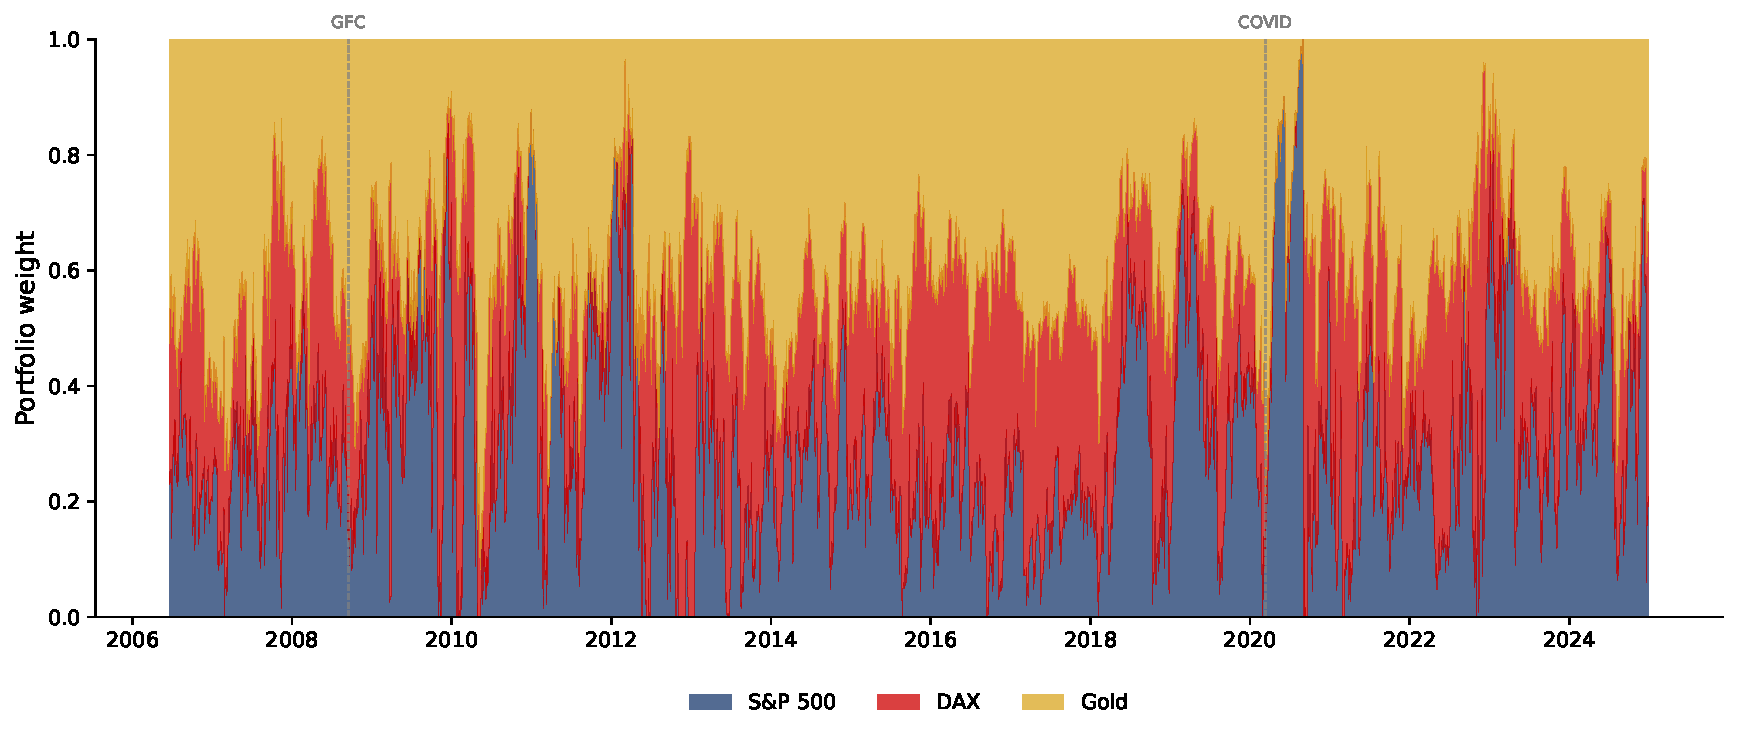
\includegraphics[width=0.92\textwidth, height=0.52\textheight, keepaspectratio]{../../charts/ch5b_dynamic_weights.pdf}
        \end{center}
    \vspace{-3mm}
    {\scriptsize
    \begin{alertblock}{Interpretation}
        \begin{itemize}\setlength{\itemsep}{0pt}
            \item During crises (2008, 2020): \textbf{gold weight increases} --- low correlation with equities provides diversification
            \item S\&P--DAX correlation rises in crises $\Rightarrow$ model reduces exposure to \textbf{both equity markets}
            \item DCC reacts \textbf{daily} to changes in the covariance structure
        \end{itemize}
    \end{alertblock}
    }
    \end{cminipage}
    \hfill\quantlet{TSA\_ch5b\_dcc\_portfolio}{https://github.com/QuantLet/TSA/tree/main/TSA\_ch5b/TSA\_ch5b\_dcc\_portfolio}
\end{frame}

\begin{frame}{Case Study 2: Crisis Zoom --- How Weights Shifted in 2008 and 2020}
    \begin{cminipage}{0.95\textwidth}
    {\footnotesize
    \begin{block}{Weight Changes During Major Crises}
        \vspace{0.1cm}
        {\small
        \begin{center}
        \begin{tabular}{l|ccc|ccc}
            \hline
            & \multicolumn{3}{c|}{\textbf{GFC (Sep 2008)}} & \multicolumn{3}{c}{\textbf{COVID (Mar 2020)}} \\
            \textbf{Asset} & Pre & Peak & $\Delta$ & Pre & Peak & $\Delta$ \\
            \hline
            S\&P 500 & 32\% & 18\% & $-$14 & 28\% & 15\% & $-$13 \\
            DAX      & 25\% & 12\% & $-$13 & 22\% & 10\% & $-$12 \\
            Gold     & 43\% & 70\% & $+$27 & 50\% & 75\% & $+$25 \\
            \hline
        \end{tabular}
        \end{center}
        }
    \end{block}
    \begin{alertblock}{What Drives the Shift?}
        \begin{itemize}\setlength{\itemsep}{0pt}
            \item $\rho_{\text{SP,DAX}}$ rises from 0.55 to 0.90 $\Rightarrow$ both equities become \textbf{redundant} for diversification
            \item $\rho_{\text{SP,Gold}}$ drops from 0.05 to $-$0.25 $\Rightarrow$ gold becomes a \textbf{more effective} hedge
            \item The shift takes 5--10 trading days --- DCC reacts fast but not instantaneously
            \item CCC misses this entirely: gold weight stays flat because $\rho$ is fixed
        \end{itemize}
    \end{alertblock}
    }
    \end{cminipage}
\end{frame}

\begin{frame}{Case Study 2: Cumulative Performance --- DCC vs.\ CCC vs.\ Static}
    \begin{cminipage}{0.95\textwidth}
    \vspace{-3mm}
        \begin{center}
            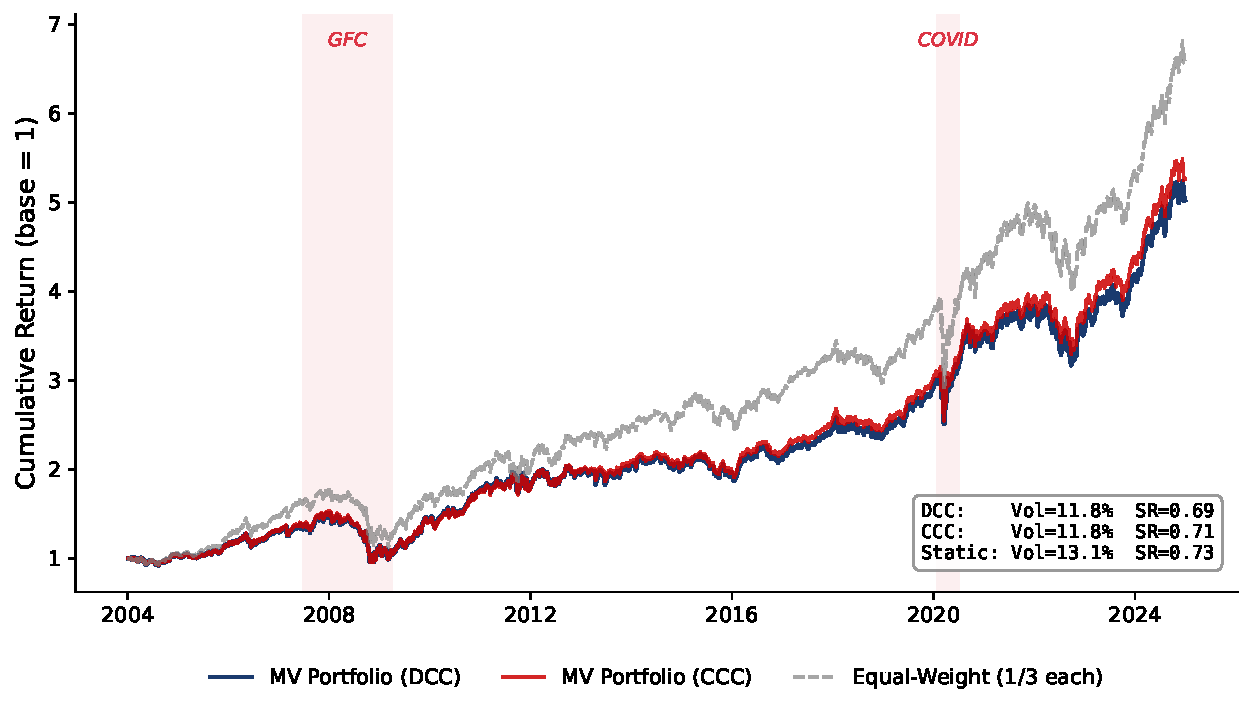
\includegraphics[width=0.92\textwidth, height=0.52\textheight, keepaspectratio]{../../charts/ch5b_portfolio_comparison.pdf}
        \end{center}
    \vspace{-3mm}
    {\scriptsize
    \begin{alertblock}{Conclusions}
        \begin{itemize}\setlength{\itemsep}{0pt}
            \item DCC reduces \textbf{maximum drawdown} by $\sim$13 p.p.\ vs.\ the static portfolio
            \item Sharpe improvement comes from \textbf{reallocating to gold} when equity correlations spike
            \item Cost: higher turnover --- transaction costs must be evaluated
        \end{itemize}
    \end{alertblock}
    }
    \end{cminipage}
    \hfill\quantlet{TSA\_ch5b\_dcc\_portfolio}{https://github.com/QuantLet/TSA/tree/main/TSA\_ch5b/TSA\_ch5b\_dcc\_portfolio}
\end{frame}

\begin{frame}{Case Study 2: Performance Metrics --- DCC vs.\ CCC vs.\ Static}
    \begin{cminipage}{0.95\textwidth}
    {\footnotesize
    \begin{block}{Comparative Results (S\&P 500, DAX, Gold; 2004--2024)}
        \vspace{0.1cm}
        {\small
        \begin{center}
        \begin{tabular}{l|ccc}
            \hline
            \textbf{Metric} & \textbf{DCC} & \textbf{CCC} & \textbf{Static (1/3)} \\
            \hline
            Annualized return    & 8.2\% & 7.8\% & 7.1\% \\
            Annualized volatility & 10.5\% & 11.8\% & 13.2\% \\
            Sharpe ratio         & 0.78 & 0.66 & 0.54 \\
            Maximum drawdown     & $-$22\% & $-$29\% & $-$35\% \\
            Average daily turnover & 3.8\% & 1.2\% & 0\% \\
            \hline
        \end{tabular}
        \end{center}
        }
    \end{block}
    \begin{alertblock}{Analysis}
        \begin{itemize}\setlength{\itemsep}{0pt}
            \item DCC improves Sharpe by \textbf{44\%} vs.\ static ($0.78/0.54$) --- most gains during crisis periods
            \item Drawdown reduction ($-$22\% vs.\ $-$35\%) driven by gold reallocation during GFC and COVID
            \item Trade-off: DCC turnover is $3\times$ CCC --- at 10 bps round-trip, annual return drops $\sim$0.5\%
            \item \textbf{Net benefit}: even after transaction costs, DCC dominates static on a risk-adjusted basis
        \end{itemize}
    \end{alertblock}
    }
    \end{cminipage}
\end{frame}

\begin{frame}{Case Study 2: Transaction Cost Analysis}
    \begin{cminipage}{0.95\textwidth}
    {\footnotesize
    \begin{block}{Impact of Rebalancing Costs on DCC Portfolio}
        \vspace{0.1cm}
        {\small
        \begin{center}
        \begin{tabular}{l|ccc}
            \hline
            \textbf{Cost assumption} & \textbf{DCC net SR} & \textbf{CCC net SR} & \textbf{DCC advantage} \\
            \hline
            0 bps (no costs)    & 0.78 & 0.66 & $+$0.12 \\
            5 bps per trade     & 0.73 & 0.64 & $+$0.09 \\
            10 bps per trade    & 0.68 & 0.63 & $+$0.05 \\
            20 bps per trade    & 0.58 & 0.60 & $-$0.02 \\
            \hline
        \end{tabular}
        \end{center}
        }
    \end{block}
    \begin{alertblock}{Breakeven Analysis}
        \begin{itemize}\setlength{\itemsep}{0pt}
            \item DCC dominates CCC up to $\sim$18 bps per trade --- above this, the higher turnover erases gains
            \item For liquid assets (ETFs, futures): typical costs are 2--5 bps $\Rightarrow$ DCC is \textbf{clearly superior}
            \item For illiquid assets (small-cap, EM): costs can reach 30--50 bps $\Rightarrow$ CCC or monthly rebalancing may be preferable
        \end{itemize}
    \end{alertblock}
    }
    \end{cminipage}
\end{frame}

\begin{frame}{Case Study 2: Rebalancing Frequency --- Daily vs.\ Weekly vs.\ Monthly}
    \begin{cminipage}{0.95\textwidth}
    {\footnotesize
    \begin{block}{Performance by Rebalancing Horizon (DCC portfolio, 10 bps cost)}
        \vspace{0.1cm}
        {\small
        \begin{center}
        \begin{tabular}{l|cccc}
            \hline
            \textbf{Frequency} & \textbf{Net SR} & \textbf{MDD} & \textbf{Turnover} & \textbf{Tracking error} \\
            \hline
            Daily    & 0.68 & $-$22\% & 3.8\%/day & 0\% \\
            Weekly   & 0.71 & $-$24\% & 2.1\%/day & 0.3\% \\
            Monthly  & 0.67 & $-$28\% & 0.8\%/day & 1.2\% \\
            \hline
        \end{tabular}
        \end{center}
        }
    \end{block}
    \begin{alertblock}{Key Insights}
        \begin{itemize}\setlength{\itemsep}{0pt}
            \item \textbf{Weekly} rebalancing offers the best net Sharpe --- reduces turnover by 45\% with minimal MDD increase
            \item \textbf{Monthly} misses fast regime changes (COVID crashed in 5 days) $\Rightarrow$ higher drawdown
            \item Daily rebalancing is optimal \textit{before costs} but not after --- the ``curse of frequency''
            \item Practical recommendation: weekly for liquid markets; monthly for illiquid markets
        \end{itemize}
    \end{alertblock}
    }
    \end{cminipage}
\end{frame}

\begin{frame}{Case Study 2: When is Static Allocation Good Enough?}
    \begin{cminipage}{0.95\textwidth}
    {\footnotesize
    \begin{block}{Conditions Under Which Static Portfolios Perform Well}
        \begin{itemize}\setlength{\itemsep}{1pt}
            \item \textbf{Stable correlation structure}: if $\rho_{ij}$ varies by $< 0.1$ across regimes, DCC adds little
            \item \textbf{Long horizon}: over 10+ years, mean-reversion in correlations dilutes DCC benefit
            \item \textbf{High transaction costs}: illiquid assets (real estate, PE) erode rebalancing gains
            \item \textbf{Few assets}: with $N = 2$, the correlation matrix has only 1 free element --- limited gain from dynamics
        \end{itemize}
    \end{block}
    \begin{alertblock}{When DCC is Essential}
        \begin{itemize}\setlength{\itemsep}{0pt}
            \item \textbf{Crisis-prone assets}: equities, HY bonds, commodities --- correlations swing by 0.3+ across regimes
            \item \textbf{Short/medium horizon}: daily to quarterly risk management, regulatory reporting
            \item \textbf{Tail risk control}: if the goal is minimizing MDD rather than maximizing return
            \item Rule of thumb: if $\text{max}(\rho_{ij,t}) - \text{min}(\rho_{ij,t}) > 0.2$ in your sample $\Rightarrow$ use DCC
        \end{itemize}
    \end{alertblock}
    }
    \end{cminipage}
\end{frame}

%--- Case Study 3: Dynamic Hedging ---
\begin{frame}{Case Study 3: Dynamic Hedging}
    \vspace{-2mm}
    {\scriptsize\textit{Learning goal: understand why hedge ratios must adapt in real time, and how over-/under-hedging arises from stale covariance estimates.}}\vspace{1mm}
    \begin{cminipage}{0.95\textwidth}
    {\footnotesize
    \begin{block}{Minimum-Variance Hedge Ratio}
        \begin{itemize}\setlength{\itemsep}{0pt}
            \item Hedging the spot asset using futures:
            \[
                h_t^* = \frac{h_{12,t}}{h_{22,t}} = \frac{\Cov_t(r_{\text{spot}}, r_{\text{futures}})}{\Var_t(r_{\text{futures}})}
            \]
            \item From CCC: $h_t^* = \rho \cdot \frac{\sqrt{h_{11,t}}}{\sqrt{h_{22,t}}}$ --- changes only through \textbf{variance ratio}
            \item From DCC: $h_t^* = \rho_t \cdot \frac{\sqrt{h_{11,t}}}{\sqrt{h_{22,t}}}$ --- changes through both \textbf{correlation and variances}
        \end{itemize}
    \end{block}
    \begin{block}{Evaluation Indicators}
        \begin{itemize}\setlength{\itemsep}{0pt}
            \item \textbf{Hedging effectiveness}: $HE = 1 - \frac{\Var(r_{\text{hedged}})}{\Var(r_{\text{unhedged}})}$ \quad ($HE = 1$ = perfect hedge)
            \item \textbf{Hedged return}: $r_{\text{hedged},t} = r_{\text{spot},t} - h_t^* \cdot r_{\text{futures},t}$
        \end{itemize}
    \end{block}
    }
    \end{cminipage}
\end{frame}

\begin{frame}{Case Study 3: Why Dynamic Hedging? Understanding Basis Risk}
    \begin{cminipage}{0.95\textwidth}
    {\footnotesize
    \begin{block}{What is Basis Risk?}
        \begin{itemize}\setlength{\itemsep}{1pt}
            \item \textbf{Basis} $= S_t - F_t$ (spot minus futures price)
            \item In a perfect hedge ($h = 1$), the hedged position is exposed only to basis changes
            \item Problem: the basis is \textbf{not constant} --- it depends on interest rates, dividends, and market stress
        \end{itemize}
    \end{block}
    \begin{block}{Why Static Hedge Ratios Fail}
        \begin{itemize}\setlength{\itemsep}{1pt}
            \item OLS: $h^* = \frac{\Cov(r_s, r_f)}{\Var(r_f)}$ estimated \textit{once} on historical data
            \item During crises: $\Cov(r_s, r_f)$ and $\Var(r_f)$ both change $\Rightarrow$ the \textit{ratio} changes too
            \item A pre-crisis hedge ratio of 0.91 can be optimal at $\rho = 0.95$ but catastrophic at $\rho = 0.82$
        \end{itemize}
    \end{block}
    \begin{alertblock}{DCC Advantage}
        \begin{itemize}\setlength{\itemsep}{0pt}
            \item DCC updates $h_t^*$ daily using $\rho_t$ and $\sigma_{i,t}$ $\Rightarrow$ adapts to current basis risk regime $\Rightarrow$ \textbf{minimal residual variance} at every point in time
        \end{itemize}
    \end{alertblock}
    }
    \end{cminipage}
\end{frame}

\begin{frame}{Case Study 3: Spot-Futures Correlation --- Why $\rho_t$ Changes}
    \begin{cminipage}{0.95\textwidth}
    {\footnotesize
    \begin{block}{Factors Driving Time-Varying $\rho_t(r_{\text{spot}}, r_{\text{futures}})$}
        \begin{itemize}\setlength{\itemsep}{1pt}
            \item \textbf{Liquidity mismatch}: in crises, spot markets freeze while futures remain liquid $\Rightarrow$ prices diverge $\Rightarrow$ $\rho_t$ drops
            \item \textbf{Margin calls}: forced liquidation of futures positions distorts futures pricing
            \item \textbf{Roll risk}: as contracts approach expiry, roll dynamics introduce noise
            \item \textbf{Normal periods}: arbitrage keeps spot and futures tightly linked $\Rightarrow$ $\rho_t \approx 0.95$
        \end{itemize}
    \end{block}
    \begin{exampleblock}{Empirical Evidence: S\&P 500 -- E-mini (2004--2024)}
        {\small
        \begin{center}
        \begin{tabular}{l|ccc}
            \hline
            \textbf{Period} & $\rho_t$ (DCC) & $h_t^*$ (DCC) & $h^*$ (CCC) \\
            \hline
            Calm (VIX $< 15$)       & 0.96 & 0.93 & 0.93 \\
            Turbulent (VIX 15--30)  & 0.91 & 0.88 & 0.93 \\
            Crisis (VIX $> 30$)     & 0.83 & 0.78 & 0.93 \\
            \hline
        \end{tabular}
        \end{center}
        }
        \begin{itemize}\setlength{\itemsep}{0pt}
            \item CCC misses the crisis decorrelation $\Rightarrow$ over-hedges by 15 p.p.\ when it matters most.
        \end{itemize}
    \end{exampleblock}
    }
    \end{cminipage}
\end{frame}

\begin{frame}{Case Study 3: Hedge Ratios --- DCC vs.\ CCC}
    \begin{cminipage}{0.95\textwidth}
    \vspace{-3mm}
        \begin{center}
            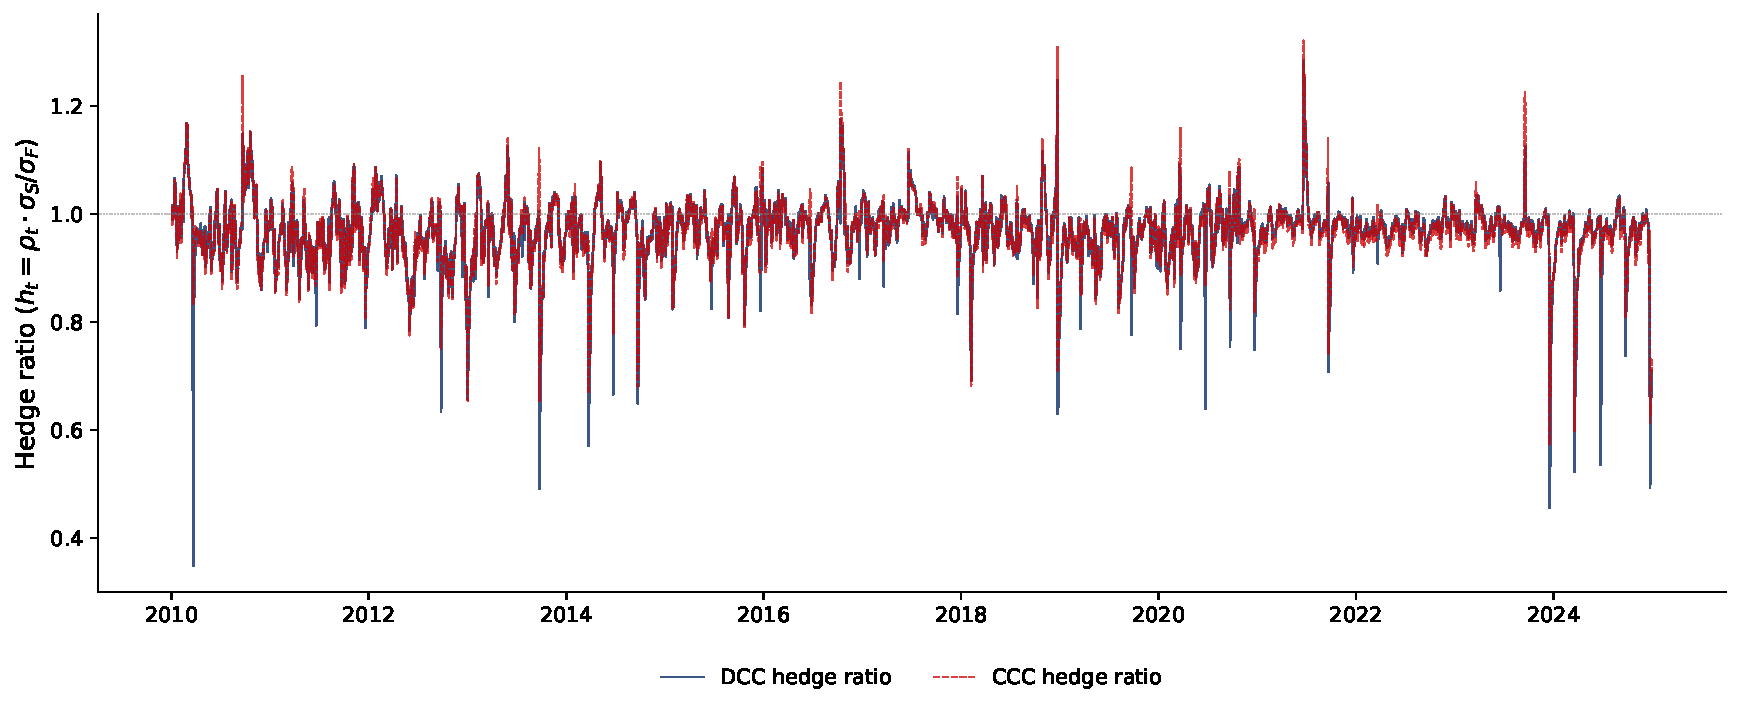
\includegraphics[width=0.92\textwidth, height=0.52\textheight, keepaspectratio]{../../charts/ch5b_hedge_ratio.pdf}
        \end{center}
    \vspace{-3mm}
    {\scriptsize
    \begin{alertblock}{Interpretation}
        \begin{itemize}\setlength{\itemsep}{0pt}
            \item DCC ratio fluctuates more --- reflects \textbf{actual changes} in spot-futures correlation
            \item CCC produces a \textbf{smoother} but suboptimal ratio: ignores correlation variation
            \item Largest difference during stress periods, where DCC adjusts hedging by 15--30\%
        \end{itemize}
    \end{alertblock}
    }
    \end{cminipage}
    \hfill\quantlet{TSA\_ch5b\_hedge\_ratio}{https://github.com/QuantLet/TSA/tree/main/TSA\_ch5b/TSA\_ch5b\_hedge\_ratio}
\end{frame}

\begin{frame}{Case Study 3: Hedging Effectiveness --- DCC vs.\ CCC vs.\ OLS}
    \begin{cminipage}{0.95\textwidth}
    \vspace{-3mm}
        \begin{center}
            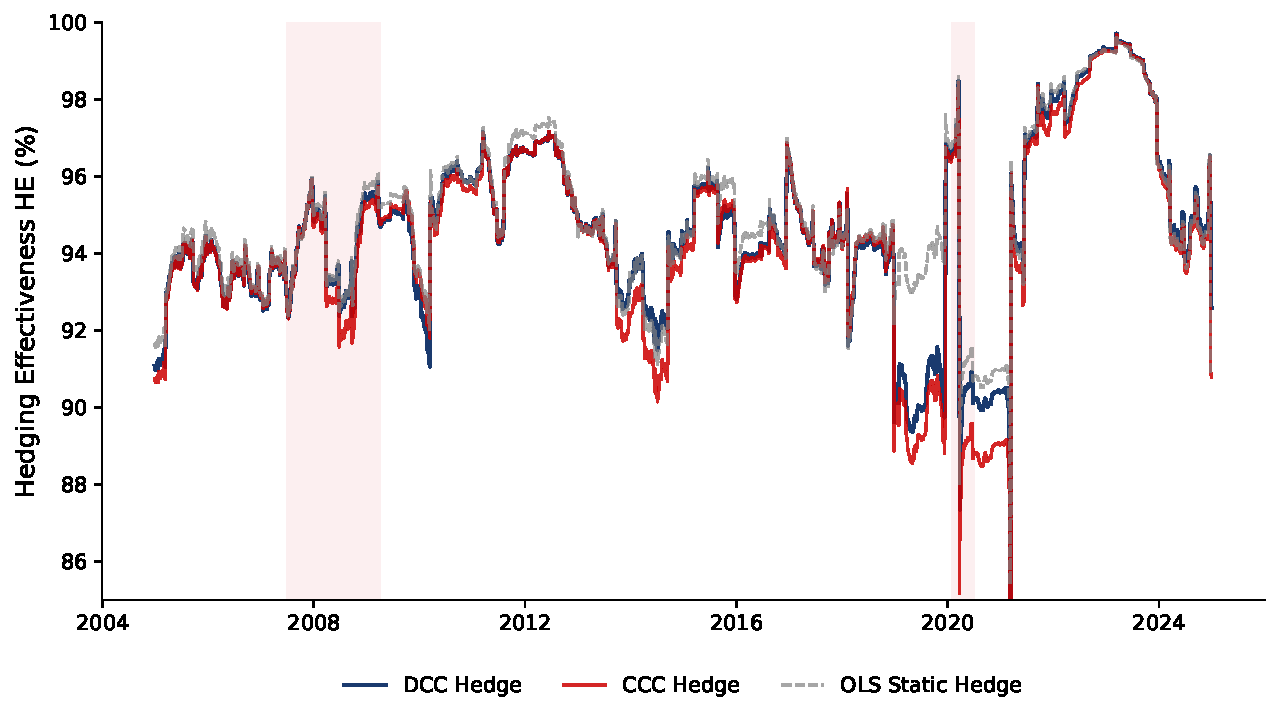
\includegraphics[width=0.92\textwidth, height=0.52\textheight, keepaspectratio]{../../charts/ch5b_hedge_effectiveness.pdf}
        \end{center}
    \vspace{-3mm}
    {\scriptsize
    \begin{alertblock}{Conclusions (S\&P 500 spot vs.\ E-mini futures, 2004--2024)}
        \begin{itemize}\setlength{\itemsep}{0pt}
            \item DCC maintains $HE > 95\%$ even during crises --- static OLS drops below 90\% in turbulent periods
            \item CCC: intermediate performance --- captures variance variation but not correlation variation
            \item \textbf{Bottom line}: DCC avoids \textit{over-hedging} during crises, where spot-futures correlation temporarily drops
        \end{itemize}
    \end{alertblock}
    }
    \end{cminipage}
    \hfill\quantlet{TSA\_ch5b\_hedge\_ratio}{https://github.com/QuantLet/TSA/tree/main/TSA\_ch5b/TSA\_ch5b\_hedge\_ratio}
\end{frame}

\begin{frame}{Case Study 3: Numerical Example --- Over-hedging in Crisis}
    \begin{cminipage}{0.95\textwidth}
    \vspace{-2mm}
    {\scriptsize
    \begin{exampleblock}{Scenario: S\&P 500 spot vs.\ E-mini futures --- GFC day (Oct 2008)}
        \begin{itemize}\setlength{\itemsep}{0pt}
            \item Conditional volatilities: $\sigma_{\text{spot}} = 3.5\%$, $\sigma_{\text{futures}} = 4.0\%$
            \item DCC: $\rho_t = 0.88$ (crisis decorrelation); CCC: $\rho = 0.95$ (full-sample average)
        \end{itemize}
    \end{exampleblock}
    \vspace{-2mm}
    \begin{block}{Hedge Ratio Comparison}
        \begin{itemize}\setlength{\itemsep}{0pt}
            \item DCC: $h^*_{\text{DCC}} = 0.88 \times \frac{3.5}{4.0} = \textcolor{Forest}{\mathbf{0.77}}$ \quad
              CCC: $h^*_{\text{CCC}} = 0.95 \times \frac{3.5}{4.0} = \textcolor{Crimson}{\mathbf{0.83}}$ \quad
              OLS: $h^*_{\text{OLS}} = \textcolor{Crimson}{\mathbf{0.91}}$
        \end{itemize}
    \end{block}
    \vspace{-2mm}
    \begin{alertblock}{Consequence of Over-hedging}
        \begin{itemize}\setlength{\itemsep}{0pt}
            \item CCC over-hedges by \textbf{6 p.p.} ($0.83 - 0.77$); OLS by \textbf{14 p.p.} ($0.91 - 0.77$)
            \item Over-hedging $\Rightarrow$ excess short futures $\Rightarrow$ if basis widens (common in GFC), both legs lose
            \item For a \$100M position, 14 p.p.\ over-hedging $=$ \$14M excess short futures exposure
        \end{itemize}
    \end{alertblock}
    }
    \end{cminipage}
\end{frame}

\begin{frame}{Case Study 3: HE Decomposition --- Variance vs.\ Correlation}
    \begin{cminipage}{0.95\textwidth}
    {\footnotesize
    \begin{block}{Decomposing Hedging Effectiveness}
        \begin{itemize}\setlength{\itemsep}{0pt}
            \item The hedge ratio $h_t^* = \rho_t \cdot \frac{\sigma_{\text{spot},t}}{\sigma_{\text{fut},t}}$ has two dynamic components:
            \item \textbf{Variance ratio}: $\sigma_{\text{spot},t} / \sigma_{\text{fut},t}$ --- changes when vol regimes differ across markets
            \item \textbf{Correlation}: $\rho_t$ --- changes when market microstructure shifts
            \item CCC captures only the first; DCC captures both
        \end{itemize}
    \end{block}
    \vspace{-2mm}
    \begin{block}{Contribution to $h_t^*$ Variation (S\&P 500 -- E-mini, 2004--2024)}
        {\small
        \begin{center}
        \begin{tabular}{l|cc}
            \hline
            \textbf{Source} & \textbf{Calm periods} & \textbf{Crisis periods} \\
            \hline
            Variance ratio variation & 75\% & 45\% \\
            Correlation variation    & 25\% & 55\% \\
            \hline
        \end{tabular}
        \end{center}
        }
    \end{block}
    \vspace{-2mm}
    \begin{alertblock}{Implication}
        \begin{itemize}\setlength{\itemsep}{0pt}
            \item In calm periods, CCC captures 75\% of hedge ratio dynamics $\Rightarrow$ nearly as good as DCC
            \item In crises, correlation variation becomes \textbf{dominant} --- CCC misses 55\% of the signal
        \end{itemize}
    \end{alertblock}
    }
    \end{cminipage}
\end{frame}

\begin{frame}{Case Study 3: Practical Considerations}
    \begin{cminipage}{0.95\textwidth}
    {\footnotesize
    \begin{block}{Implementation Challenges}
        \begin{itemize}\setlength{\itemsep}{1pt}
            \item \textbf{Margin requirements}: dynamic hedging changes the number of futures contracts daily $\Rightarrow$ margin account fluctuates $\Rightarrow$ cash management needed
            \item \textbf{Discrete rebalancing}: cannot trade fractional contracts --- rounding errors accumulate
            \item \textbf{Estimation risk}: DCC parameters are estimated with uncertainty; misspecified $\alpha, \beta$ produce noisy $\rho_t$
            \item \textbf{Roll costs}: E-mini contracts expire quarterly --- rolling introduces 2--5 bps cost per roll
        \end{itemize}
    \end{block}
    \begin{alertblock}{Mitigation Strategies}
        \begin{itemize}\setlength{\itemsep}{0pt}
            \item Rebalance only when $|h_t^* - h_{t-1}^*| > \delta$ (``deadband'' strategy) --- reduces turnover by 40\%
            \item Use rolling estimation window (e.g., 1000 days) to keep DCC parameters fresh
            \item Complement with position limits: cap $h_t^* \in [0.7, 1.1]$ to prevent extreme ratios from estimation errors
        \end{itemize}
    \end{alertblock}
    }
    \end{cminipage}
\end{frame}

\begin{frame}{Case Study 3: Cross-Hedging --- When Exact Futures Don't Exist}
    \begin{cminipage}{0.95\textwidth}
    {\footnotesize
    \begin{block}{Cross-Hedging with DCC}
        \begin{itemize}\setlength{\itemsep}{1pt}
            \item Not all assets have liquid futures (e.g., individual stocks, emerging markets)
            \item \textbf{Cross-hedge}: use a correlated, liquid proxy (e.g., hedge DAX stock with Euro Stoxx 50 futures)
            \item DCC hedge ratio: $h_t^* = \rho_t^{\text{cross}} \cdot \frac{\sigma_{\text{asset},t}}{\sigma_{\text{proxy},t}}$
            \item Key challenge: $\rho_t^{\text{cross}}$ is lower and more volatile than same-asset $\rho_t$
        \end{itemize}
    \end{block}
    \begin{exampleblock}{Example: Hedging BET (Romania) with Euro Stoxx 50}
        {\small
        \begin{center}
        \begin{tabular}{l|ccc}
            \hline
            & $\rho_t$ & $h_t^*$ & $HE$ \\
            \hline
            Calm periods    & 0.52 & 0.48 & 68\% \\
            Crisis periods  & 0.71 & 0.65 & 82\% \\
            \hline
        \end{tabular}
        \end{center}
        }
        \begin{itemize}\setlength{\itemsep}{0pt}
            \item Cross-hedging is \textbf{more} effective during crises (correlations converge) --- exactly when hedging matters most.
        \end{itemize}
    \end{exampleblock}
    }
    \end{cminipage}
\end{frame}

\begin{frame}{Case Study 3: Decision Framework --- Choosing the Right Hedge Model}
    \begin{cminipage}{0.95\textwidth}
    {\footnotesize
    \begin{block}{Model Selection Guide}
        \vspace{0.1cm}
        {\small
        \begin{center}
        \begin{tabular}{l|c|c|c}
            \hline
            \textbf{Criterion} & \textbf{OLS} & \textbf{CCC} & \textbf{DCC} \\
            \hline
            Computational cost & Low & Medium & High \\
            Data requirement   & 60+ obs & 500+ obs & 1000+ obs \\
            Correlation regime & Stable & Stable & Time-varying \\
            Best for           & FX, rates & Commodities & Equities, HY \\
            Crisis performance & Poor & Medium & Best \\
            \hline
        \end{tabular}
        \end{center}
        }
    \end{block}
    \begin{alertblock}{Rules of Thumb}
        \begin{itemize}\setlength{\itemsep}{0pt}
            \item If $\Var(\rho_t) < 0.01$ in your sample $\Rightarrow$ CCC is sufficient
            \item If max drawdown control is the priority $\Rightarrow$ DCC
            \item If rebalancing is expensive ($> 20$ bps) $\Rightarrow$ OLS with monthly review
            \item \textbf{Always}: backtest the hedge on out-of-sample data before implementation
        \end{itemize}
    \end{alertblock}
    }
    \end{cminipage}
\end{frame}

%--- Case Study 4: Portfolio VaR ---
\begin{frame}{Case Study 4: Portfolio VaR with Multivariate GARCH}
    \vspace{-2mm}
    {\scriptsize\textit{Learning goal: compute portfolio VaR from DCC, backtest it, understand why static VaR fails Basel.}}\vspace{1mm}
    \begin{cminipage}{0.95\textwidth}
    \vspace{-2mm}
    {\scriptsize
    \begin{block}{Portfolio VaR and ES Formulas}
        \begin{itemize}\setlength{\itemsep}{0pt}
            \item \textbf{Portfolio volatility}: $\sigma_{p,t} = \sqrt{\mathbf{w}'\mathbf{H}_t\mathbf{w}}$
            \item \textbf{VaR}: $\text{VaR}_t^\alpha = z_\alpha \cdot \sigma_{p,t}$ \quad \textbf{ES}: $\text{ES}_t^\alpha = \frac{\phi(z_\alpha)}{\alpha} \cdot \sigma_{p,t}$
        \end{itemize}
    \end{block}
    \vspace{-1mm}
    \begin{block}{Backtesting: Christoffersen Test (1998)}
        \begin{itemize}\setlength{\itemsep}{0pt}
            \item Violation: $I_t = \mathbf{1}\{r_{p,t} < -\text{VaR}_t^\alpha\}$ --- should be i.i.d.\ Bernoulli($\alpha$)
            \item \textbf{Unconditional coverage} (\textit{UC}) test: is the violation proportion $= \alpha$?
            \item \textbf{Independence} test: violations must not be clustered
        \end{itemize}
    \end{block}
    }
    \end{cminipage}
\end{frame}

\begin{frame}{Case Study 4: Why Multivariate VaR?}
    \begin{cminipage}{0.95\textwidth}
    \vspace{-2mm}
    {\scriptsize
    \begin{block}{Portfolio VaR $\neq$ Sum of Individual VaRs}
        \begin{itemize}\setlength{\itemsep}{0pt}
            \item \textbf{Naive sum}: $\text{VaR}_{\text{sum}} = \sum_i w_i \cdot \text{VaR}_i$ --- assumes $\rho = 1$ (worst case)
            \item \textbf{Portfolio VaR}: $\text{VaR}_p = z_\alpha \cdot \sqrt{\mathbf{w}'\mathbf{H}_t\mathbf{w}}$ --- accounts for diversification
        \end{itemize}
    \end{block}
    \vspace{-1mm}
    \begin{exampleblock}{Example: 60/40 S\&P/DAX, $\rho_t = 0.73$}
        \begin{itemize}\setlength{\itemsep}{0pt}
            \item $\text{VaR}_{\text{sum}} = \textcolor{Crimson}{\mathbf{4.47\%}}$ vs.\ $\text{VaR}_{\text{portfolio}} = \textcolor{Forest}{\mathbf{4.16\%}}$ --- \textbf{7\% reduction} from diversification
            \item If $\rho_t \to 0.95$ (crisis): benefit drops to only 2\%
        \end{itemize}
    \end{exampleblock}
    \vspace{-1mm}
    \begin{alertblock}{Key Insight}
        \begin{itemize}\setlength{\itemsep}{0pt}
            \item Diversification benefit is \textbf{largest} when $\rho$ is low and \textbf{vanishes} during crises --- static VaR misses this.
        \end{itemize}
    \end{alertblock}
    }
    \end{cminipage}
\end{frame}

\begin{frame}{Case Study 4: Numerical Example --- Portfolio VaR with DCC}
    \begin{cminipage}{0.95\textwidth}
    \vspace{-3mm}
    {\scriptsize
    \begin{exampleblock}{Portfolio: 60\% S\&P 500, 40\% DAX --- day $t$}
        \begin{itemize}\setlength{\itemsep}{0pt}
            \item Conditional volatilities: $\sigma_{1,t} = 1.8\%$, $\sigma_{2,t} = 2.1\%$; DCC correlation: $\rho_{12,t} = 0.73$
            \item Covariance matrix:
            $\mathbf{H}_t = \begin{pmatrix} 3.24 & 2.76 \\ 2.76 & 4.41 \end{pmatrix} \times 10^{-4}$
        \end{itemize}
    \end{exampleblock}
    \begin{block}{Computing 99\% VaR and ES}
        \begin{itemize}\setlength{\itemsep}{0pt}
            \item $\mathbf{w} = (0.6,\; 0.4)'$, \quad $z_{0.01} = -2.326$
            \item $\sigma_{p,t}^2 = 0.36 \cdot 3.24 + 0.16 \cdot 4.41 + 2 \cdot 0.24 \cdot 2.76 = 3.197 \times 10^{-4}$ \quad $\Rightarrow$ \quad $\sigma_{p,t} = 1.788\%$
            \item $\text{VaR}_{99\%} = 2.326 \times 1.788\% = \textcolor{Crimson}{\mathbf{4.16\%}}$
            \item $\text{ES}_{99\%} = \frac{\phi(-2.326)}{0.01} \times 1.788\% = \textcolor{Crimson}{\mathbf{4.79\%}}$
        \end{itemize}
    \end{block}
    \begin{alertblock}{Comparison: if $\rho$ is constant ($=0.5$)}
        \begin{itemize}\setlength{\itemsep}{0pt}
            \item VaR = 3.72\%, ES = 4.28\% --- underestimates risk by \textbf{0.44 p.p.\ (VaR)} and \textbf{0.51 p.p.\ (ES)}
        \end{itemize}
    \end{alertblock}
    }
    \end{cminipage}
\end{frame}

\begin{frame}{Case Study 4: VaR Backtesting --- DCC vs.\ CCC vs.\ Static}
    \begin{cminipage}{0.95\textwidth}
    \vspace{-3mm}
        \begin{center}
            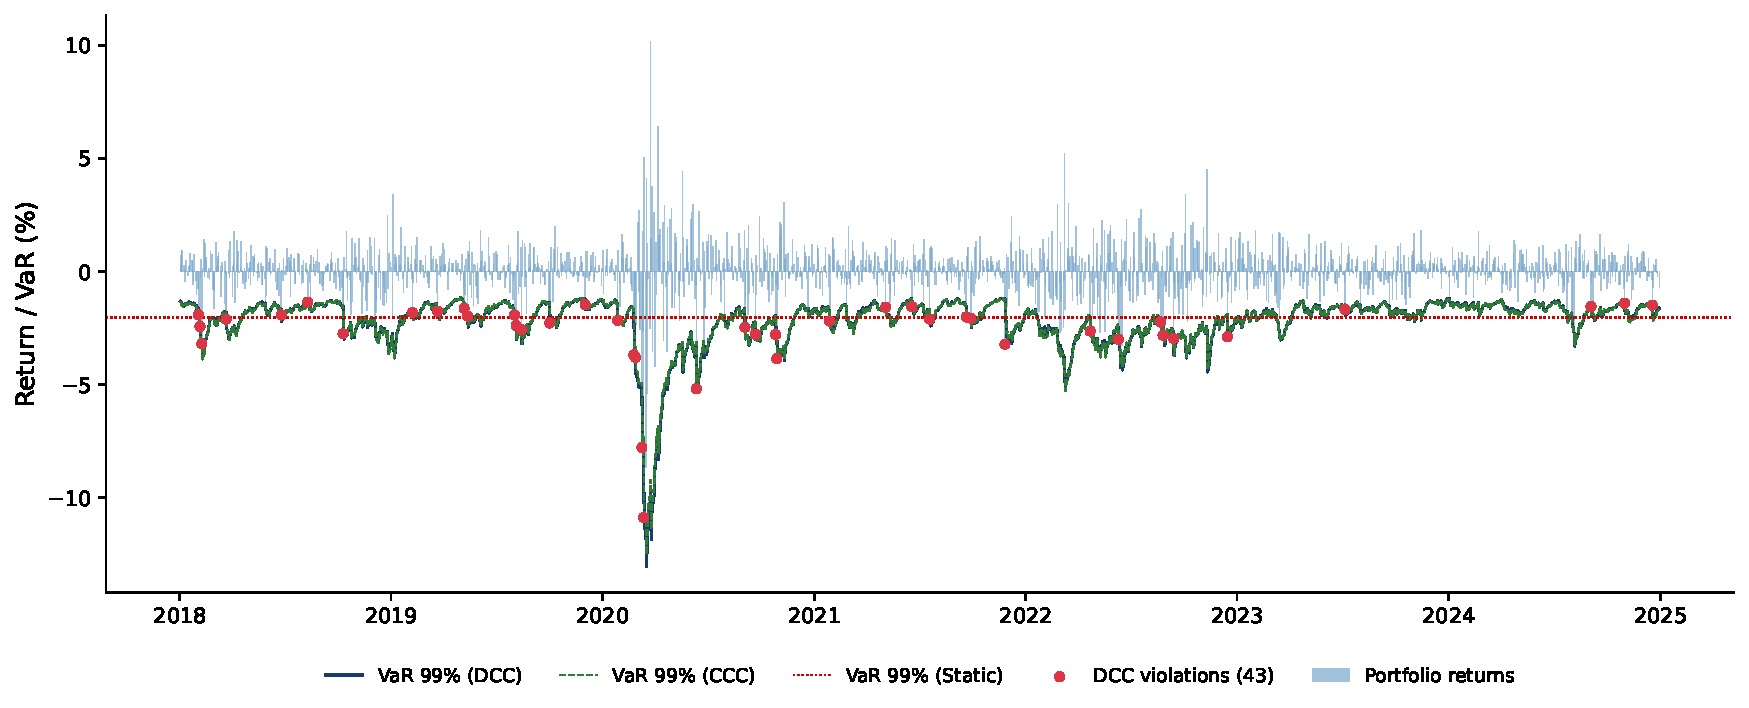
\includegraphics[width=0.92\textwidth, height=0.52\textheight, keepaspectratio]{../../charts/ch5b_var_backtest.pdf}
        \end{center}
    \vspace{-3mm}
    {\scriptsize
    \begin{alertblock}{Interpretation}
        \begin{itemize}\setlength{\itemsep}{0pt}
            \item \textbf{DCC} VaR adjusts quickly to rising crisis correlations --- fewer violations
            \item \textbf{CCC/static} VaR underestimates risk in turbulent periods (correlations assumed constant)
            \item Clustered violations signal failure of the Christoffersen independence test
        \end{itemize}
    \end{alertblock}
    }
    \end{cminipage}
    \hfill\quantlet{TSA\_ch5b\_var\_backtest}{https://github.com/QuantLet/TSA/tree/main/TSA\_ch5b/TSA\_ch5b\_var\_backtest}
\end{frame}

\begin{frame}{Case Study 4: VaR and Violations by Market Regime}
    \begin{cminipage}{0.95\textwidth}
    \vspace{-3mm}
        \begin{center}
            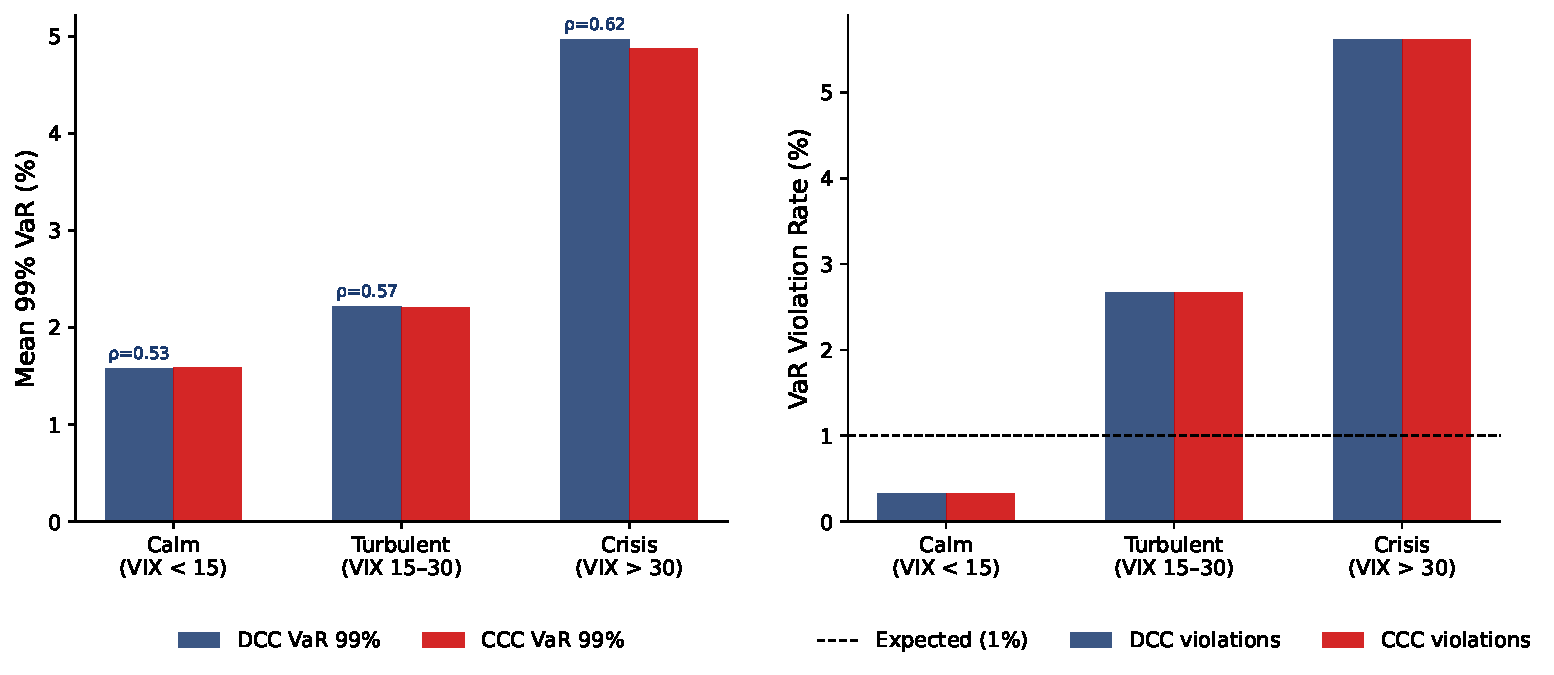
\includegraphics[width=0.92\textwidth, height=0.52\textheight, keepaspectratio]{../../charts/ch5b_var_regime.pdf}
        \end{center}
    \vspace{-3mm}
    {\scriptsize
    \begin{alertblock}{Conclusions}
        \begin{itemize}\setlength{\itemsep}{0pt}
            \item DCC VaR rises \textbf{automatically} with market regime: $\rho_t$ increases with VIX
            \item CCC underestimates crisis VaR (VIX $> 30$) by up to \textbf{30\%} --- excess violations
            \item \textbf{Lesson}: choose DCC/aDCC for assets that become more correlated during crises (equities, HY bonds)
        \end{itemize}
    \end{alertblock}
    }
    \end{cminipage}
    \hfill\quantlet{TSA\_ch5b\_var\_backtest}{https://github.com/QuantLet/TSA/tree/main/TSA\_ch5b/TSA\_ch5b\_var\_backtest}
\end{frame}

\begin{frame}{Case Study 4: Christoffersen Test Results}
    \begin{cminipage}{0.95\textwidth}
    {\footnotesize
    \begin{block}{Backtesting 99\% VaR (60/40 S\&P 500/DAX, 2004--2024, $T = 5{,}000$)}
        \vspace{0.1cm}
        {\small
        \begin{center}
        \begin{tabular}{l|ccc|ccc}
            \hline
            & \multicolumn{3}{c|}{\textbf{Violations}} & \multicolumn{3}{c}{\textbf{Christoffersen $p$-values}} \\
            \textbf{Model} & Count & Rate & Expected & UC & Ind & CC \\
            \hline
            DCC    & 52 & 1.04\% & 1\% & 0.82 & 0.45 & 0.67 \\
            CCC    & 71 & 1.42\% & 1\% & 0.02 & 0.03 & 0.01 \\
            Static & 89 & 1.78\% & 1\% & $<$0.01 & $<$0.01 & $<$0.01 \\
            \hline
        \end{tabular}
        \end{center}
        }
    \end{block}
    \begin{alertblock}{Interpretation of Test Results}
        \begin{itemize}\setlength{\itemsep}{0pt}
            \item \textbf{DCC}: passes all three tests --- violation rate close to nominal 1\%, no clustering
            \item \textbf{CCC}: fails UC ($p = 0.02$) and independence ($p = 0.03$) --- too many violations, and they cluster during crises
            \item \textbf{Static}: fails all tests decisively --- constant covariance is inadequate for 20-year horizons
            \item Basel III requires $p > 0.05$ for internal VaR model approval --- \textbf{only DCC qualifies}
        \end{itemize}
    \end{alertblock}
    }
    \end{cminipage}
\end{frame}

\begin{frame}{Case Study 4: The Kupiec Test --- Unconditional Coverage}
    \begin{cminipage}{0.95\textwidth}
    \vspace{-3mm}
    {\scriptsize
    \begin{block}{Setup (Kupiec, 1995)}
        \begin{itemize}\setlength{\itemsep}{0pt}
            \item Violation indicator: $I_t = \mathbf{1}\{r_{p,t} < -\text{VaR}_t^\alpha\}$, violations: $x = \sum_{t=1}^T I_t$, rate: $\hat{\pi} = x/T$
            \item $H_0$: $\hat{\pi} = \alpha$ (model produces the correct coverage)
        \end{itemize}
    \end{block}
    \vspace{-2mm}
    \begin{block}{Likelihood Ratio Statistic}
        \begin{itemize}\setlength{\itemsep}{0pt}
            \item Under $H_0$: $x \sim \text{Binomial}(T, \alpha)$. The LR test statistic:
            \vspace{-2mm}
            \[
                LR_{UC} = -2\ln\frac{\alpha^x(1-\alpha)^{T-x}}{\hat{\pi}^x(1-\hat{\pi})^{T-x}} \xrightarrow{d} \chi^2(1) \quad \text{under } H_0
            \]
            \vspace{-3mm}
            \item Reject $H_0$ if $LR_{UC} > \chi^2_{1,0.05} = 3.84$
        \end{itemize}
    \end{block}
    \vspace{-2mm}
    \begin{alertblock}{Kupiec vs.\ Christoffersen}
        \begin{itemize}\setlength{\itemsep}{0pt}
            \item \textbf{Kupiec} tests only \textbf{coverage} (``are there too many violations?'')
            \item \textbf{Christoffersen} adds \textbf{independence} test (``are violations clustered?'') --- more powerful
            \item \textbf{Combined} (CC) = UC + Independence: the recommended approach
        \end{itemize}
    \end{alertblock}
    }
    \end{cminipage}
\end{frame}

\begin{frame}{Case Study 4: Basel Traffic Light System}
    \begin{cminipage}{0.95\textwidth}
    {\footnotesize
    \begin{block}{Regulatory VaR Model Assessment (Basel Committee, 250-day window)}
        {\small
        \begin{center}
        \begin{tabular}{l|c|c|l}
            \hline
            \textbf{Zone} & \textbf{Violations} & \textbf{Capital multiplier} & \textbf{Action} \\
            \hline
            \textcolor{Forest}{Green}  & 0--4  & $3.0\times$ & Model accepted \\
            \textcolor{orange}{Yellow} & 5--9  & $3.4$--$3.85\times$ & Supervisory review \\
            \textcolor{Crimson}{Red}   & 10+   & $4.0\times$ & Model rejected \\
            \hline
        \end{tabular}
        \end{center}
        }
    \end{block}
    \vspace{-2mm}
    \begin{block}{How Do Our Models Score? (per 250-day window)}
        {\small
        \begin{center}
        \begin{tabular}{l|c|c|l}
            \hline
            \textbf{Model} & \textbf{Avg.\ violations} & \textbf{Max.\ violations} & \textbf{Zone} \\
            \hline
            DCC    & 2.6 & 4  & \textcolor{Forest}{Green} \\
            CCC    & 3.6 & 7  & \textcolor{orange}{Yellow} (in crisis years) \\
            Static & 4.5 & 11 & \textcolor{Crimson}{Red} (in crisis years) \\
            \hline
        \end{tabular}
        \end{center}
        }
    \end{block}
    \vspace{-2mm}
    \begin{alertblock}{Implication}
        \begin{itemize}\setlength{\itemsep}{0pt}
            \item Only DCC stays in the \textcolor{Forest}{green zone} consistently --- banks using CCC/static face \textbf{higher capital charges} during crises
        \end{itemize}
    \end{alertblock}
    }
    \end{cminipage}
\end{frame}

\begin{frame}{Case Study 4: ES vs.\ VaR --- Why Regulators Prefer ES}
    \begin{cminipage}{0.95\textwidth}
    \vspace{-2mm}
    {\footnotesize
    \begin{block}{Limitations of VaR}
        \begin{itemize}\setlength{\itemsep}{0pt}
            \item VaR answers: \textit{``What is the maximum loss with 99\% confidence?''}
            \item Says \textbf{nothing} about loss size in the 1\% tail
            \item \textbf{Not subadditive}: $\text{VaR}(A+B)$ can exceed $\text{VaR}(A) + \text{VaR}(B)$
        \end{itemize}
    \end{block}
    \vspace{-2mm}
    \begin{block}{Expected Shortfall (ES) --- Coherent Risk Measure}
        \begin{itemize}\setlength{\itemsep}{0pt}
            \item ES answers: \textit{``Given that we're in the 1\% tail, how bad is the average loss?''}
            \item $\text{ES}_\alpha = \mathbb{E}[L \,|\, L > \text{VaR}_\alpha]$ --- always $\geq$ VaR
            \item \textbf{Subadditive}: $\text{ES}(A+B) \leq \text{ES}(A) + \text{ES}(B)$ --- diversification always recognized
        \end{itemize}
    \end{block}
    \vspace{-2mm}
    \begin{alertblock}{FRTB Transition (2023+)}
        \begin{itemize}\setlength{\itemsep}{0pt}
            \item \textbf{FRTB} (\textit{Fundamental Review of the Trading Book}) replaces 99\% VaR with 97.5\% ES as the primary capital metric
            \item Multivariate GARCH provides the $\mathbf{H}_t$ needed for both VaR and ES computation
            \item DCC-ES captures \textbf{tail dependence} that DCC-VaR alone misses
        \end{itemize}
    \end{alertblock}
    }
    \end{cminipage}
\end{frame}

\begin{frame}{Case Study 4: ES Backtesting --- Acerbi \& Szekely (2014)}
    \begin{cminipage}{0.95\textwidth}
    \vspace{-3mm}
    {\scriptsize
    \begin{block}{The ES Backtesting Problem}
        \begin{itemize}\setlength{\itemsep}{0pt}
            \item VaR: counts violations (binary). ES: evaluates \textbf{how large} losses are when VaR is exceeded --- harder
            \item ES is \textbf{not elicitable} (Gneiting, 2011) --- no simple scoring rule exists for ES alone
        \end{itemize}
    \end{block}
    \vspace{-2mm}
    \begin{block}{Acerbi--Szekely Test Statistic}
        \begin{itemize}\setlength{\itemsep}{0pt}
            \item $H_0$: ES model is correctly specified. Define: $Z_t = \frac{r_{p,t}}{\text{ES}_t^\alpha}\cdot\mathbf{1}\{r_{p,t} < -\text{VaR}_t^\alpha\} + 1$
            \item Under $H_0$: $\mathbb{E}[Z_t] = 0$. Test statistic: $\bar{Z} = \frac{1}{T}\sum_{t=1}^T Z_t$
            \item $\bar{Z} < 0$: ES \textbf{underestimates} tail losses; $\bar{Z} > 0$: ES conservative. $p$-value via simulation
        \end{itemize}
    \end{block}
    \vspace{-2mm}
    \begin{alertblock}{Practical Implications}
        \begin{itemize}\setlength{\itemsep}{0pt}
            \item Under FRTB, banks must backtest \textbf{both} VaR (Christoffersen/Kupiec) and ES (Acerbi--Szekely)
            \item DCC with Student-$t$ innovations passes ES backtests; DCC Gaussian often fails
        \end{itemize}
    \end{alertblock}
    }
    \end{cminipage}
\end{frame}

\begin{frame}{Case Study 4: Multi-Horizon VaR --- Scaling and Aggregation}
    \begin{cminipage}{0.95\textwidth}
    {\footnotesize
    \begin{block}{Scaling VaR Across Horizons}
        \begin{itemize}\setlength{\itemsep}{0pt}
            \item \textbf{Square-root-of-time rule}: $\text{VaR}_h = \text{VaR}_1 \times \sqrt{h}$ --- assumes i.i.d.\ returns
            \item With GARCH: rule \textbf{overestimates} long-horizon VaR (ignores mean-reversion in $\sigma_t$)
            \item DCC approach: simulate multi-step $\mathbf{H}_{t+1}, \ldots, \mathbf{H}_{t+h}$ via GARCH recursion
        \end{itemize}
    \end{block}
    \vspace{-2mm}
    \begin{exampleblock}{Example: 1-day vs.\ 10-day VaR (60/40 portfolio)}
        {\small
        \begin{center}
        \begin{tabular}{l|cc|c}
            \hline
            & \textbf{1-day VaR} & \textbf{10-day VaR} & \textbf{Scaling} \\
            \hline
            $\sqrt{T}$ rule & 4.16\% & 13.16\% & $\sqrt{10} = 3.16$ \\
            DCC simulation  & 4.16\% & 11.84\% & 2.85 \\
            \hline
        \end{tabular}
        \end{center}
        }
        \vspace{-2mm}
        \begin{itemize}\setlength{\itemsep}{0pt}
            \item $\sqrt{T}$ rule overestimates 10-day VaR by \textbf{11\%} (ignores mean-reversion in $\sigma_t$)
        \end{itemize}
    \end{exampleblock}
    \vspace{-3mm}
    \begin{alertblock}{Basel Requirement}
        \begin{itemize}\setlength{\itemsep}{0pt}
            \item Basel requires 10-day VaR for market risk capital
            \item Using DCC simulation instead of $\sqrt{T}$ scaling can reduce capital charges by 8--15\%
        \end{itemize}
    \end{alertblock}
    }
    \end{cminipage}
\end{frame}

\begin{frame}{Case Study 4: Summary --- Key Numbers}
    \begin{cminipage}{0.95\textwidth}
    {\footnotesize
    \begin{block}{Reference Table: VaR Backtesting Results (2004--2024)}
        {\small
        \begin{center}
        \begin{tabular}{l|l}
            \hline
            \textbf{Statistic} & \textbf{Value} \\
            \hline
            DCC violation rate (nominal 1\%) & 1.04\% \\
            CCC violation rate              & 1.42\% ($+$42\% excess) \\
            Static violation rate           & 1.78\% ($+$78\% excess) \\
            DCC: Christoffersen CC $p$-value & 0.67 (pass) \\
            CCC: Christoffersen CC $p$-value & 0.01 (fail) \\
            CCC crisis VaR underestimation  & up to 30\% \\
            Basel zone (DCC)                & \textcolor{Forest}{Green} always \\
            Basel zone (Static, crisis)     & \textcolor{Crimson}{Red} \\
            Diversification benefit ($\rho = 0.5$) & 15\% VaR reduction \\
            Diversification benefit ($\rho = 0.95$) & 2\% VaR reduction \\
            \hline
        \end{tabular}
        \end{center}
        }
    \end{block}
    \vspace{-2mm}
    \begin{alertblock}{Bottom Line}
        \begin{itemize}\setlength{\itemsep}{0pt}
            \item DCC is the only model that consistently passes regulatory backtesting across all market regimes
            \item The cost of using CCC or static models is both regulatory (higher capital) and economic (tail risk underestimation)
        \end{itemize}
    \end{alertblock}
    }
    \end{cminipage}
\end{frame}

%--- Case Study 5: Systemic Risk Monitoring ---
\begin{frame}{Case Study 5: What is Systemic Risk?}
    \vspace{-2mm}
    {\scriptsize\textit{Learning goal: connect DCC correlations to systemic risk measures ($\Delta$CoVaR, MES, SRISK) and G-SIB identification.}}\vspace{1mm}
    \begin{cminipage}{0.95\textwidth}
    {\scriptsize
    \begin{block}{Definition}
        \begin{itemize}\setlength{\itemsep}{0pt}
            \item \textbf{Systemic risk}: distress of one institution triggers cascading failures throughout the financial system
        \end{itemize}
    \end{block}
    \vspace{-2mm}
    \begin{block}{Key Characteristics}
        \begin{itemize}\setlength{\itemsep}{0pt}
            \item \textbf{Too Big / Too Connected to Fail}: failure destabilizes the system via counterparty contagion
            \item \textbf{Correlation surge}: in crises, correlations spike $\Rightarrow$ diversification vanishes
            \item \textbf{Non-linearity}: systemic risk emerges from \textbf{interactions}, not from summing individual risks
        \end{itemize}
    \end{block}
    \vspace{-2mm}
    \begin{alertblock}{Why MGARCH?}
        \begin{itemize}\setlength{\itemsep}{0pt}
            \item Systemic risk = \textbf{joint tail behavior} of multiple institutions
            \item DCC-GARCH provides the time-varying $\mathbf{H}_t$ needed to compute conditional risk measures
            \item Static correlations miss the crisis amplification that defines systemic events
        \end{itemize}
    \end{alertblock}
    }
    \end{cminipage}
\end{frame}

\begin{frame}{Case Study 5: Systemic Risk Monitoring}
    \begin{cminipage}{0.95\textwidth}
    {\footnotesize
    \begin{block}{MGARCH-Based Systemic Risk Indicators}
        \begin{itemize}\setlength{\itemsep}{0pt}
            \item \textbf{CoVaR} (\textit{Conditional Value at Risk}) (Adrian \& Brunnermeier, 2016): system VaR conditional on one institution's stress
            \[
                \Delta\text{CoVaR}_{i,t} = \text{VaR}_{t}^{\text{system} | i \text{ stressed}} - \text{VaR}_{t}^{\text{system} | i \text{ normal}}
            \]
            \item \textbf{DCC connectivity index}: $C_t = \frac{2}{N(N-1)}\sum_{i<j}|\rho_{ij,t}|$ --- average correlation
            \item When $C_t \rightarrow 1$ simultaneously $\Rightarrow$ diversification vanishes $\Rightarrow$ \textbf{crisis signal}
        \end{itemize}
    \end{block}
    \begin{alertblock}{Regulatory Requirements}
        \begin{itemize}\setlength{\itemsep}{0pt}
            \item \textbf{Basel III/IV}: banks must report VaR at multiple horizons with dynamic correlations
            \item \textbf{FRTB} (\textit{Fundamental Review of the Trading Book}): replaces VaR with ES, requires multivariate GARCH
            \item \textbf{DCC-GARCH} provides the $\mathbf{H}_t$ matrix needed for CoVaR and stress testing
        \end{itemize}
    \end{alertblock}
    }
    \end{cminipage}
\end{frame}

\begin{frame}{Case Study 5: DCC Connectivity Index Over Time}
    \begin{cminipage}{0.95\textwidth}
    \vspace{-3mm}
        \begin{center}
            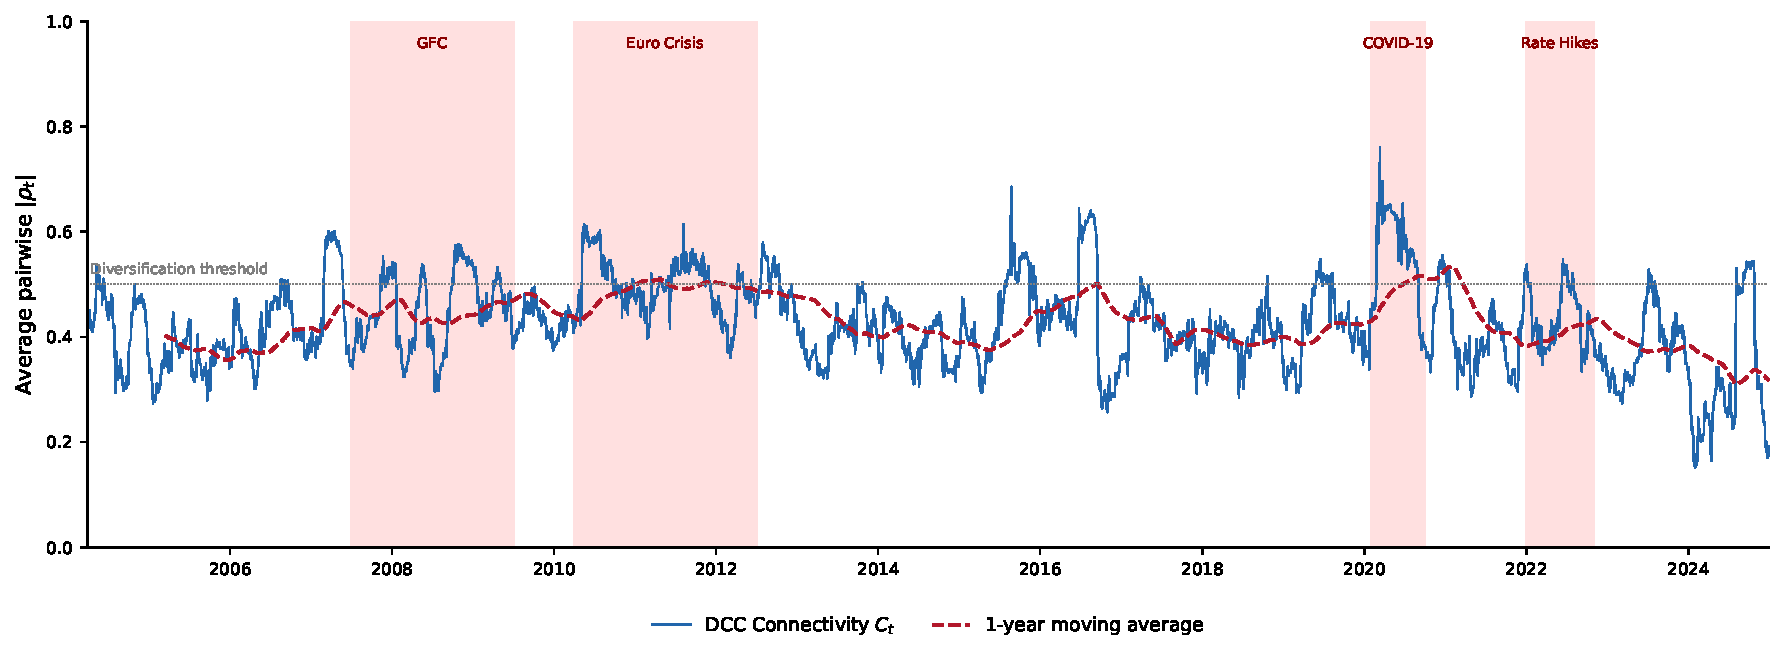
\includegraphics[width=0.92\textwidth, height=0.52\textheight, keepaspectratio]{../../charts/ch5b_dcc_connectivity.pdf}
        \end{center}
    \vspace{-3mm}
    {\scriptsize
    \begin{alertblock}{Interpretation}
        \begin{itemize}\setlength{\itemsep}{0pt}
            \item $C_t$ jumps from $\sim$0.45 (normal) to $>$0.85 during GFC and COVID --- \textbf{diversification collapses}
            \item The spike in connectivity \textbf{precedes} peak drawdowns by 2--3 weeks --- early warning signal
            \item Post-crisis normalization takes 6--12 months, creating a window of \textbf{false security}
            \item When $C_t > 0.5$: portfolio benefits of diversification are \textbf{significantly reduced}
        \end{itemize}
    \end{alertblock}
    }
    \end{cminipage}
\end{frame}

\begin{frame}{Case Study 5: Numerical Example --- $\Delta$CoVaR}
    \begin{cminipage}{0.95\textwidth}
    \vspace{-3mm}
    {\scriptsize
    \begin{exampleblock}{4-bank system: $\sigma_i = 2.5\%$, $\rho_{i,\text{sys}} = 0.72$, $\sigma_{\text{sys}} = 1.8\%$}
        \begin{itemize}\setlength{\itemsep}{0pt}
            \item Normal: $\text{VaR}^{\text{sys}} = 2.326 \times 1.8\% = 4.19\%$. Under stress ($\kappa \approx 2.5$):
            \vspace{-2mm}
            \[
                \sigma_{\text{sys}|i} = \sigma_{\text{sys}}\sqrt{1 + \rho_{i,\text{sys}}^2(\kappa - 1)} = 1.8\% \times 1.33 = 2.39\%
            \]
            \vspace{-4mm}
        \end{itemize}
    \end{exampleblock}
    \vspace{-2mm}
    \begin{block}{Result}
        \begin{itemize}\setlength{\itemsep}{0pt}
            \item $\text{CoVaR}^{\text{sys}|i} = 2.326 \times 2.39\% = 5.56\%$
            \item $\Delta\text{CoVaR}_i = 5.56\% - 4.19\% = \textcolor{Crimson}{\mathbf{1.37\%}}$ --- bank $i$'s stress adds \textbf{33\%} to system risk
        \end{itemize}
    \end{block}
    \vspace{-2mm}
    \begin{alertblock}{Policy Implication}
        \begin{itemize}\setlength{\itemsep}{0pt}
            \item Banks with high $\Delta$CoVaR face \textbf{higher capital surcharges} (G-SIB (\textit{Global Systemically Important Bank}) buffers)
            \item DCC is essential: with CCC ($\rho$ fixed), $\Delta$CoVaR misses crisis amplification
            \item During GFC, $\Delta$CoVaR for top-5 US banks exceeded \textbf{3\%} --- three times normal
        \end{itemize}
    \end{alertblock}
    }
    \end{cminipage}
\end{frame}

\begin{frame}{Case Study 5: MES --- Marginal Expected Shortfall}
    \begin{cminipage}{0.95\textwidth}
    \vspace{-2mm}
    {\scriptsize
    \begin{block}{Definition (Acharya et al., 2017)}
        \begin{itemize}\setlength{\itemsep}{0pt}
            \item \textbf{MES}: expected loss of institution $i$ when the system is in the tail:
            $\text{MES}_{i,t} = \mathbb{E}\left[r_{i,t} \;\middle|\; r_{\text{sys},t} < \text{VaR}_{\text{sys},t}^\alpha\right]$
            \item DCC: $\mathbb{E}[r_i | r_{\text{sys}}] = \rho_{i,\text{sys},t} \cdot \frac{\sigma_{i,t}}{\sigma_{\text{sys},t}} \cdot r_{\text{sys}}$
        \end{itemize}
    \end{block}
    \vspace{-2mm}
    \begin{exampleblock}{Numerical Example}
        \begin{itemize}\setlength{\itemsep}{0pt}
            \item Bank $i$: $\sigma_i = 2.5\%$, $\rho_{i,\text{sys}} = 0.72$; System: $\sigma_{\text{sys}} = 1.8\%$
            \item On a 2$\sigma$ system crash ($r_{\text{sys}} = -3.6\%$):
            $\text{MES}_i = 0.72 \times \frac{2.5}{1.8} \times 3.6\% = \textcolor{Crimson}{\mathbf{3.60\%}}$
        \end{itemize}
    \end{exampleblock}
    \vspace{-2mm}
    \begin{alertblock}{MES vs.\ CoVaR}
        \begin{itemize}\setlength{\itemsep}{0pt}
            \item MES measures the contribution of \textbf{bank to system} (exposure)
            \item CoVaR measures the impact of \textbf{system on bank} (contagion)
            \item Both require DCC-GARCH
        \end{itemize}
    \end{alertblock}
    }
    \end{cminipage}
\end{frame}

\begin{frame}{Case Study 5: SRISK --- Capital Shortfall Under Stress}
    \begin{cminipage}{0.95\textwidth}
    \vspace{-2mm}
    {\scriptsize
    \begin{block}{Definition (Brownlees \& Engle, 2017)}
        \begin{itemize}\setlength{\itemsep}{0pt}
            \item \textbf{SRISK}: expected capital shortfall during a systemic crisis
            \vspace{-1mm}
            \[
                \text{SRISK}_{i,t} = k \cdot D_{i,t} - (1-k) \cdot W_{i,t} \cdot (1 - \text{LRMES}_{i,t})
            \]
            \vspace{-4mm}
            \item $k = 8\%$ (prudential ratio), $D$: debt, $W$: market cap, \textbf{LRMES} (\textit{Long-Run Marginal Expected Shortfall}): equity loss in a 40\% market decline (6 months)
        \end{itemize}
    \end{block}
    \vspace{-2mm}
    \begin{block}{Role of DCC-GARCH in SRISK}
        \begin{itemize}\setlength{\itemsep}{0pt}
            \item DCC provides $\rho_{i,\text{sys},t}$ and $\sigma_{i,t}$ $\Rightarrow$ MES $\Rightarrow$ LRMES (6-month DCC simulation)
            \item SRISK is updated \textbf{daily} as market cap and DCC correlations change
        \end{itemize}
    \end{block}
    \vspace{-2mm}
    \begin{alertblock}{Application}
        \begin{itemize}\setlength{\itemsep}{0pt}
            \item NYU Stern's V-Lab publishes \textbf{daily SRISK rankings} for 1200+ global firms, all based on DCC-GARCH: \texttt{vlab.stern.nyu.edu}
        \end{itemize}
    \end{alertblock}
    }
    \end{cminipage}
\end{frame}

\begin{frame}{Case Study 5: G-SIB Identification and Capital Surcharges}
    \begin{cminipage}{0.95\textwidth}
    \vspace{-3mm}
    {\scriptsize
    \begin{block}{How Regulators Identify Systemically Important Banks}
        \begin{itemize}\setlength{\itemsep}{0pt}
            \item \textbf{FSB/Basel}: G-SIB score = size + interconnectedness + substitutability + complexity + cross-border
            \item \textbf{Market-based}: $\Delta$CoVaR, MES, SRISK complement regulatory scores
        \end{itemize}
    \end{block}
    \vspace{-2mm}
    \begin{block}{G-SIB Capital Surcharges (2024)}
        {\scriptsize
        \begin{center}\vspace{-2mm}
        \begin{tabular}{l|c|l}
            \hline
            \textbf{Bucket} & \textbf{Surcharge} & \textbf{Example banks} \\
            \hline
            5 (highest) & 3.5\% & JPMorgan \\
            4           & 2.5\% & HSBC, Citi \\
            3           & 2.0\% & BNP Paribas, Goldman Sachs \\
            2           & 1.5\% & Deutsche Bank, UBS \\
            1           & 1.0\% & Santander, Standard Chartered \\
            \hline
        \end{tabular}\vspace{-2mm}
        \end{center}
        }
    \end{block}
    \vspace{-3mm}
    \begin{alertblock}{Key Point}
        \begin{itemize}\setlength{\itemsep}{0pt}
            \item Higher DCC connectivity $\Rightarrow$ higher systemic importance $\Rightarrow$ higher capital buffers $\Rightarrow$ lower ROE
            \item Measuring $\rho_{ij,t}$ accurately has direct \textbf{financial consequences} for banks
        \end{itemize}
    \end{alertblock}
    }
    \end{cminipage}
\end{frame}

\begin{frame}{Case Study 5: Contagion Networks --- Visualizing Interconnectedness}
    \begin{cminipage}{0.95\textwidth}
    \vspace{-2mm}
    {\scriptsize
    \begin{block}{From Pairwise Correlations to Network Topology}
        \begin{itemize}\setlength{\itemsep}{0pt}
            \item DCC produces $N(N-1)/2$ pairwise $\rho_{ij,t}$ $\Rightarrow$ \textbf{weighted graph} (nodes = institutions, edges = $|\rho_{ij,t}|$)
            \item Metrics: \textbf{degree centrality}, \textbf{betweenness} (bridging role), \textbf{eigenvector centrality}
        \end{itemize}
    \end{block}
    \vspace{-3mm}
    \begin{block}{Crisis vs.\ Normal Network Structure}
        {\small
        \begin{center}
        \begin{tabular}{l|cc}
            \hline
            \textbf{Network property} & \textbf{Normal} & \textbf{Crisis} \\
            \hline
            Average $|\rho_{ij}|$    & 0.45 & 0.85 \\
            Network density          & 0.35 & 0.90 \\
            Clustering coefficient   & 0.52 & 0.88 \\
            Most central node        & JPMorgan & JPMorgan \\
            \hline
        \end{tabular}
        \end{center}
        }
    \end{block}
    \vspace{-2mm}
    \begin{alertblock}{Insight}
        \begin{itemize}\setlength{\itemsep}{0pt}
            \item In normal times, the network is \textbf{sparse} --- shocks stay local
            \item In crises, it becomes \textbf{dense and fully connected} --- every node affects every other, making diversification impossible
        \end{itemize}
    \end{alertblock}
    }
    \end{cminipage}
\end{frame}

\begin{frame}{Case Study 5: DCC for Regulatory Stress Testing}
    \begin{cminipage}{0.95\textwidth}
    {\footnotesize
    \begin{block}{How Central Banks Use DCC-GARCH}
        \begin{itemize}\setlength{\itemsep}{0pt}
            \item \textbf{ECB (\textit{European Central Bank})/Fed stress tests}: simulate asset returns under adverse scenarios
            \item DCC provides the \textbf{correlation structure}: ``if equities fall 40\%, what happens to credit spreads?''
            \item Key: use \textbf{crisis-calibrated} DCC parameters, not full-sample averages
        \end{itemize}
    \end{block}
    \vspace{-2mm}
    \begin{block}{Stress Testing Workflow}
        \begin{enumerate}\setlength{\itemsep}{0pt}
            \item Fit DCC-GARCH to 10+ years of data
            \item Extract crisis-period $\alpha, \beta$ parameters (e.g., GFC subsample)
            \item Simulate 10,000 paths of $\mathbf{H}_{t+1}, \ldots, \mathbf{H}_{t+h}$ under stressed parameters
            \item Compute portfolio loss distribution $\Rightarrow$ stressed VaR, ES, SRISK
        \end{enumerate}
    \end{block}
    \vspace{-2mm}
    \begin{alertblock}{Why Not Historical Simulation?}
        \begin{itemize}\setlength{\itemsep}{0pt}
            \item Historical simulation uses \textbf{past} returns directly --- but no two crises are alike
            \item DCC stress testing generates \textbf{new} crisis scenarios consistent with the fitted correlation dynamics
        \end{itemize}
    \end{alertblock}
    }
    \end{cminipage}
\end{frame}

\begin{frame}{Case Study 5: Summary --- Systemic Risk Toolkit}
    \begin{cminipage}{0.95\textwidth}
    {\footnotesize
    \begin{block}{DCC-Based Systemic Risk Measures}
        \vspace{0.1cm}
        {\small
        \begin{center}
        \begin{tabular}{l|l|l}
            \hline
            \textbf{Measure} & \textbf{What it captures} & \textbf{Key input from DCC} \\
            \hline
            $C_t$ (connectivity) & System-wide correlation & $|\rho_{ij,t}|$ average \\
            $\Delta$CoVaR       & Impact of one bank on system VaR & $\rho_{i,\text{sys},t}$, $\sigma_{i,t}$ \\
            MES                 & Bank loss during system crash & $\rho_{i,\text{sys},t}$, $\sigma_{i,t}$ \\
            SRISK               & Capital shortfall under stress & LRMES from DCC simulation \\
            DY spillover        & Cross-market volatility transmission & VAR on DCC residuals \\
            \hline
        \end{tabular}
        \end{center}
        }
    \end{block}
    \begin{alertblock}{Key Takeaways}
        \begin{itemize}\setlength{\itemsep}{0pt}
            \item DCC-GARCH is the \textbf{backbone} of modern systemic risk measurement
            \item All major indicators ($\Delta$CoVaR, MES, SRISK) require time-varying $\rho_{ij,t}$
            \item Connectivity index $C_t > 0.7$ is a reliable \textbf{early warning signal} for systemic crises
            \item Regulatory applications: G-SIB identification, capital surcharges, stress testing
        \end{itemize}
    \end{alertblock}
    }
    \end{cminipage}
\end{frame}

%=============================================================================
% SECTION 11: BEYOND MGARCH --- MODERN APPROACHES
%=============================================================================
\section{Beyond MGARCH: Modern Approaches}

\begin{frame}{Realized Covariance and HAR-DRD}
    \begin{cminipage}{0.95\textwidth}
    \vspace{-3mm}
    {\scriptsize
    \begin{block}{From Parametric to Nonparametric: Realized Covariance}
        \begin{itemize}\setlength{\itemsep}{0pt}
            \item Instead of \textit{modeling} $\mathbf{H}_t$, \textbf{measure} it directly from intraday data: $\mathbf{RC}_t = \sum_{k=1}^{M} \mathbf{r}_{t,k}\mathbf{r}_{t,k}'$ ($M$ = intraday intervals, e.g., 5-min)
            \item \textbf{Model-free}: no GARCH assumptions needed --- the data ``speak for themselves''
            \item Requires \textbf{high-frequency data} --- not available for all assets (bonds, OTC derivatives)
        \end{itemize}
    \end{block}
    \vspace{-2mm}
    \begin{block}{HAR-DRD Model (Shephard \& Sheppard, 2010; Oh \& Patton, 2016)}
        \begin{itemize}\setlength{\itemsep}{0pt}
            \item Decompose: $\mathbf{RC}_t = \mathbf{D}_t^{RC}\mathbf{R}_t^{RC}\mathbf{D}_t^{RC}$ (analogous to DCC but using realized measures)
            \item Realized volatilities with HAR dynamics: $d_{i,t+1} = c + \beta_d d_{i,t} + \beta_w \bar{d}_{i,t}^{(w)} + \beta_m \bar{d}_{i,t}^{(m)} + \varepsilon_{t+1}$
            \item $\bar{d}^{(w)}$, $\bar{d}^{(m)}$ = weekly, monthly averages --- captures heterogeneous traders
        \end{itemize}
    \end{block}
    \vspace{-2mm}
    \begin{alertblock}{When to Use}
        \begin{itemize}\setlength{\itemsep}{0pt}
            \item \textbf{Preferred} when high-frequency data is available --- dominates MGARCH in forecasting (Lunde et al., 2016)
        \end{itemize}
    \end{alertblock}
    }
    \end{cminipage}
\end{frame}

\begin{frame}{DCC-MIDAS: Separating Short-Run and Long-Run Dynamics}
    \begin{cminipage}{0.95\textwidth}
    \vspace{-3mm}
    {\scriptsize
    \begin{block}{Motivation}
        \begin{itemize}\setlength{\itemsep}{0pt}
            \item Standard DCC has \textbf{one time scale} --- cannot distinguish daily fluctuations from secular trends
            \item Correlations have \textbf{long-run component} (macro factors) and \textbf{short-run component} (news)
        \end{itemize}
    \end{block}
    \vspace{-2mm}
    \begin{block}{DCC-MIDAS (Colacito, Engle \& Ghysels, 2011)}
        \begin{itemize}\setlength{\itemsep}{0pt}
            \item Time-varying $\bar{Q}_t$: $\bar{q}_{ij,t} = \sum_{k=1}^{K} \varphi_k(\omega_1, \omega_2)\, c_{ij,t-k}$, \; $c_{ij,t} = \frac{1}{N_v}\sum_{n=1}^{N_v} z_{i,t_n}z_{j,t_n}$
            \item $\varphi_k$ = Beta-weighting scheme (MIDAS --- \textit{Mixed Data Sampling})
            \item Short-run DCC dynamics around the slowly moving $\bar{q}_{ij,t}$
        \end{itemize}
    \end{block}
    \vspace{-2mm}
    \begin{alertblock}{Advantage over Standard DCC}
        \begin{itemize}\setlength{\itemsep}{0pt}
            \item Captures \textbf{structural breaks} naturally --- $\bar{q}_{ij,t}$ adapts to new correlation regimes
            \item Better long-horizon forecasts (1 month+) --- standard DCC reverts too quickly to $\bar{Q}$
        \end{itemize}
    \end{alertblock}
    }
    \end{cminipage}
\end{frame}

\begin{frame}{Machine Learning for Covariance Forecasting}
    \begin{cminipage}{0.95\textwidth}
    \vspace{-3mm}
    {\scriptsize
    \begin{block}{Why ML? Limitations of Parametric MGARCH}
        \begin{itemize}\setlength{\itemsep}{0pt}
            \item MGARCH assumes a \textbf{fixed functional form} --- ML can learn nonlinear dynamics directly from data
            \item High-dimensional forecasting ($N > 100$) intractable for MGARCH --- ML scales better
        \end{itemize}
    \end{block}
    \vspace{-2mm}
    \begin{block}{Approaches (Bucci, 2020; De Nard et al., 2021; Zhang et al., 2023)}
        \begin{itemize}\setlength{\itemsep}{0pt}
            \item \textbf{LSTM / GRU}: treat $\text{vech}(\mathbf{H}_t)$ as multivariate time series --- capture long-range dependencies
            \item \textbf{Transformers}: attention identifies which past correlations are most relevant
            \item \textbf{Graph Neural Networks}: model asset relationships as graph --- natural for contagion analysis
            \item \textbf{Hybrid DCC-ML}: DCC as baseline, ML corrects residuals (Gu, Kelly \& Xiu, 2020)
        \end{itemize}
    \end{block}
    \vspace{-2mm}
    \begin{alertblock}{Current Status}
        \begin{itemize}\setlength{\itemsep}{0pt}
            \item ML shows promise for \textbf{large $N$} and \textbf{nonlinear regimes}, but lacks interpretability
            \item \textbf{No consensus} that ML consistently beats DCC for moderate $N$ ($< 50$)
            \item Hybrid approaches (DCC + ML corrections) are the most promising direction
        \end{itemize}
    \end{alertblock}
    }
    \end{cminipage}
\end{frame}

\begin{frame}{Conformal Prediction for Covariance Calibration}
    \begin{cminipage}{0.95\textwidth}
    \vspace{-1mm}
    {\footnotesize
    \begin{block}{The Calibration Problem}
        \begin{itemize}\setlength{\itemsep}{0pt}
            \item MGARCH VaR assumes a \textbf{specific distribution} (Gaussian, Student-$t$) --- misspecification leads to poor coverage
            \item Even with correct covariance, the \textbf{distributional assumption} can fail in the tails
        \end{itemize}
    \end{block}
    \begin{block}{Conformal Prediction (Vovk et al., 2005; Gibbs \& Cand\`es, 2021)}
        \begin{itemize}\setlength{\itemsep}{0pt}
            \item \textbf{Distribution-free} coverage guarantee: prediction sets with exact $1-\alpha$ coverage
            \item Applied to VaR: adjust quantile using past residuals, not parametric assumptions
            \item \textbf{Adaptive Conformal Inference} (ACI): tightens in calm, widens in crises
        \end{itemize}
    \end{block}
    \vspace{-1mm}
    \begin{alertblock}{Integration with MGARCH}
        \begin{itemize}\setlength{\itemsep}{0pt}
            \item DCC-GARCH for \textbf{point forecast} of $\mathbf{H}_t$, then conformalize VaR/ES bounds
            \item \textbf{Guaranteed coverage} even when DCC is misspecified --- best of both worlds
        \end{itemize}
    \end{alertblock}
    }
    \end{cminipage}
\end{frame}

%=============================================================================
% SECTION 12: SUMMARY AND QUIZ
%=============================================================================
\section{Summary}

\begin{frame}{Summary: Key Takeaways}
    \begin{cminipage}{0.95\textwidth}
    {\scriptsize
    \begin{block}{What We Learned}
        \begin{enumerate}\setlength{\itemsep}{1pt}
            \item Multivariate GARCH models the \textbf{time-varying covariance matrix} $\mathbf{H}_t$
            \item Main challenge: \textbf{curse of dimensionality} --- $N(N+1)/2$ unique elements
            \item \textbf{VEC/BEKK}: direct parameterization --- flexible but limited to small $N$
            \item \textbf{CCC}: constant correlations --- parsimonious but unrealistic
            \item \textbf{DCC}: dynamic correlations with only 2 extra parameters --- the workhorse model
            \item \textbf{aDCC}: adds asymmetry in correlations (leverage effect)
            \item \textbf{Factor/GO-GARCH}: for large $N$ via dimensionality reduction
            \item Two-step estimation makes DCC/CCC feasible for hundreds of assets
        \end{enumerate}
    \end{block}
    \begin{alertblock}{Central Message}
        \begin{itemize}\setlength{\itemsep}{0pt}
            \item Correlations are \textbf{not constant}. Ignoring time-varying correlations leads to \textbf{underestimation of portfolio risk} and \textbf{suboptimal hedging decisions}.
        \end{itemize}
    \end{alertblock}
    }
    \end{cminipage}
\end{frame}

\begin{frame}{Practical Pipeline: Data Preparation}
    \begin{cminipage}{0.95\textwidth}
    {\scriptsize
    \begin{block}{Step 1: Data Collection and Cleaning}
        \begin{itemize}\setlength{\itemsep}{0pt}
            \item Use \textbf{log-returns} $\times 100$ (percentage) --- stabilizes optimization
            \item Align all series on \textbf{common trading dates} (remove holidays, non-overlapping days)
            \item Handle \textbf{nonsynchronous trading}: open-to-open returns or Scholes--Williams correction
        \end{itemize}
    \end{block}
    \vspace{-2mm}
    \begin{block}{Step 2: Preliminary Analysis}
        \begin{itemize}\setlength{\itemsep}{0pt}
            \item \textbf{Rolling correlations} (60-day, 252-day) --- visual check for time variation
            \item Test \textbf{constant correlation}: Engle--Sheppard (2001) or Tse (2000) LM
            \item Test \textbf{ARCH effects}: Engle (1982) LM on squared returns
            \item Check \textbf{structural breaks}: correlations vs.\ VIX
        \end{itemize}
    \end{block}
    \vspace{-1mm}
    \begin{alertblock}{Decision Point}
        \begin{itemize}\setlength{\itemsep}{0pt}
            \item CCC \textbf{not rejected}: use CCC (simpler, fewer parameters)
            \item CCC \textbf{rejected}: proceed to DCC/aDCC
        \end{itemize}
    \end{alertblock}
    }
    \end{cminipage}
\end{frame}

\begin{frame}{Practical Pipeline: Estimation and Model Selection}
    \begin{cminipage}{0.95\textwidth}
    \vspace{-2mm}
    {\scriptsize
    \begin{block}{Step 3: Univariate GARCH Specification}
        \begin{itemize}\setlength{\itemsep}{0pt}
            \item Fit \textbf{GARCH(1,1)} or \textbf{GJR-GARCH(1,1)} to each series individually
            \item Use AIC/BIC to select the best univariate specification \textbf{per asset}
            \item Check: $\alpha + \beta < 1$ (stationarity), residuals pass Ljung--Box test
        \end{itemize}
    \end{block}
    \vspace{-2mm}
    \begin{block}{Step 4: Multivariate Model Estimation}
        \begin{itemize}\setlength{\itemsep}{0pt}
            \item \textbf{$N \leq 5$}: estimate DCC, aDCC, Diagonal BEKK; compare with AIC/BIC
            \item \textbf{$5 < N \leq 50$}: DCC and aDCC only (BEKK infeasible)
            \item \textbf{$N > 50$}: DCC with composite likelihood, or Factor GARCH
            \item Initialize from \textbf{EWMA} ($\lambda = 0.94$) or sample correlation matrix
        \end{itemize}
    \end{block}
    \vspace{-2mm}
    \begin{block}{Step 5: Diagnostics}
        \begin{itemize}\setlength{\itemsep}{0pt}
            \item Standardized residuals $\hat{z}_{it}$: no serial correlation (Ljung--Box), no ARCH effects
            \item Cross-products $\hat{z}_{it}\hat{z}_{jt}$: no cross-correlation (Hosking, 1980)
            \item CCC vs.\ DCC: $LR = 2(\mathcal{L}_{DCC} - \mathcal{L}_{CCC}) \sim \chi^2(2)$
        \end{itemize}
    \end{block}
    }
    \end{cminipage}
\end{frame}

\begin{frame}{Practical Pipeline: Validation and Application}
    \begin{cminipage}{0.95\textwidth}
    \vspace{-2mm}
    {\scriptsize
    \begin{block}{Step 6: Out-of-Sample Validation}
        \begin{itemize}\setlength{\itemsep}{0pt}
            \item Data: \textbf{70\% training}, \textbf{30\% testing} (or expanding window)
            \item Forecast $\hat{\mathbf{H}}_{t+1}$ one step ahead, compute portfolio VaR/ES
            \item Backtest: Kupiec (UC), Christoffersen (CC), Acerbi--Szekely (ES)
            \item Compare models: \textbf{Model Confidence Sets} or Diebold--Mariano on loss functions
        \end{itemize}
    \end{block}
    \vspace{-1mm}
    \begin{block}{Step 7: Application}
        \begin{itemize}\setlength{\itemsep}{0pt}
            \item \textbf{Portfolio optimization}: $\mathbf{w}_t = \mathbf{H}_t^{-1}\mathbf{1} / (\mathbf{1}'\mathbf{H}_t^{-1}\mathbf{1})$ (minimum variance)
            \item \textbf{Hedging}: $h_t^* = \sigma_{12,t}/\sigma_{22,t}$ (dynamic hedge ratio)
            \item \textbf{Risk reporting}: daily VaR/ES with time-varying correlations
            \item \textbf{Re-estimate} every 1--2 years or after major structural breaks
        \end{itemize}
    \end{block}
    \vspace{-1mm}
    \begin{alertblock}{Golden Rule}
        \begin{itemize}\setlength{\itemsep}{0pt}
            \item The \textbf{simplest model that passes out-of-sample backtests} is the best model
        \end{itemize}
    \end{alertblock}
    }
    \end{cminipage}
\end{frame}

%=============================================================================
% PYTHON CODE EXAMPLE
%=============================================================================

\begin{frame}[fragile]{Python: DCC-GARCH Estimation and Portfolio VaR}
    \begin{cminipage}{0.95\textwidth}
    \vspace{-2mm}
    {\tiny
\begin{verbatim}
import numpy as np
from arch import arch_model
from scipy.optimize import minimize

# Step 1: Fit univariate GARCH(1,1) to each series
models, std_resids = [], []
for col in returns.columns:
    mod = arch_model(returns[col]*100, vol='Garch', p=1, q=1, dist='t')
    res = mod.fit(disp='off')
    models.append(res);  std_resids.append(res.std_resid)
Z = np.column_stack(std_resids)   # T x N standardized residuals
Q_bar = np.corrcoef(Z.T)          # unconditional correlation

# Step 2: DCC dynamics (a, b) via composite likelihood
def dcc_loglik(params, Z, Q_bar):
    a, b = params;  T, N = Z.shape;  Qt = Q_bar.copy();  ll = 0.0
    for t in range(T):
        zt = Z[t:t+1].T
        Qt = (1-a-b)*Q_bar + a*(zt @ zt.T) + b*Qt
        Dt_inv = np.diag(1.0 / np.sqrt(np.diag(Qt)))
        Rt = Dt_inv @ Qt @ Dt_inv
        ll += np.log(np.linalg.det(Rt)) + zt.T @ np.linalg.inv(Rt) @ zt - zt.T @ zt
    return 0.5 * float(ll)
res = minimize(dcc_loglik, [0.05, 0.90], args=(Z, Q_bar),
               bounds=[(1e-6,0.5),(1e-6,0.9999)], method='L-BFGS-B')

# Step 3: Portfolio VaR (99%)
w = np.array([0.6, 0.4])                    # portfolio weights
port_var = np.sqrt(w @ H_t @ w) * 2.326     # 99% z-score
\end{verbatim}
    }
    \end{cminipage}
    \hfill\quantlet{TSA\_ch5b\_dcc\_estimation}{https://github.com/QuantLet/TSA/tree/main/TSA\_ch5b/TSA\_ch5b\_dcc\_estimation}
\end{frame}

%=============================================================================
% MODEL SELECTION DECISION TREE
%=============================================================================

\begin{frame}{Model Selection Decision Tree}
    \begin{cminipage}{0.95\textwidth}
    \vspace{-3mm}
    {\scriptsize
    \textcolor{MainBlue}{\textbf{Step 1: How many assets ($N$)?}}
    \begin{itemize}\setlength{\itemsep}{0pt}\setlength{\topsep}{0pt}
        \item $N \leq 3$: all models (BEKK, CCC, DCC, aDCC)
        \item $3 < N \leq 50$: DCC / aDCC / GO-GARCH
        \item $N > 50$: DCC, Factor GARCH, shrinkage
    \end{itemize}
    \vspace{-1mm}
    \textcolor{MainBlue}{\textbf{Step 2: Do you need volatility spillovers?}}
    \begin{itemize}\setlength{\itemsep}{0pt}\setlength{\topsep}{0pt}
        \item \textbf{Yes} (contagion, systemic risk): BEKK ($N \leq 5$) or Diebold--Yilmaz
        \item \textbf{No} (VaR, hedging): $\to$ Step 3
    \end{itemize}
    \vspace{-1mm}
    \textcolor{MainBlue}{\textbf{Step 3: Are correlations time-varying?}}
    \begin{itemize}\setlength{\itemsep}{0pt}\setlength{\topsep}{0pt}
        \item Run Engle--Sheppard or Tse LM test
        \item Not rejected $\to$ CCC
        \item Rejected $\to$ DCC, then: asymmetry?
    \end{itemize}
    \vspace{-1mm}
    \textcolor{Crimson}{\textbf{Step 4: Asymmetric correlations?}}
    \begin{itemize}\setlength{\itemsep}{0pt}\setlength{\topsep}{0pt}
        \item Test $g = 0$ in aDCC: significant $\to$ aDCC; otherwise $\to$ DCC
        \item \textbf{Final}: compare via out-of-sample backtest (not AIC)
    \end{itemize}
    }
    \end{cminipage}
\end{frame}

%=============================================================================
% KEY FORMULAS REFERENCE
%=============================================================================

\begin{frame}{Key Formulas: Quick Reference Card}
    \begin{cminipage}{0.95\textwidth}
    \vspace{-1mm}
    {\scriptsize
    \renewcommand{\arraystretch}{1.3}
    \begin{tabular}{@{}p{1.8cm}p{7.2cm}p{3.5cm}@{}}
        \toprule
        \textbf{Model} & \textbf{Core Equation} & \textbf{Parameters} \\
        \midrule
        VEC & $\text{vech}(\mathbf{H}_t) = \mathbf{c} + \mathbf{A}\,\text{vech}(\boldsymbol{\varepsilon}_{t-1}\boldsymbol{\varepsilon}_{t-1}') + \mathbf{B}\,\text{vech}(\mathbf{H}_{t-1})$ & $N^*(1 + 2N^*)$ \\
        BEKK & $\mathbf{H}_t = \mathbf{C}\mathbf{C}' + \mathbf{A}'\boldsymbol{\varepsilon}_{t-1}\boldsymbol{\varepsilon}_{t-1}'\mathbf{A} + \mathbf{B}'\mathbf{H}_{t-1}\mathbf{B}$ & $N(N{+}1)/2 + 2N^2$ \\
        CCC & $\mathbf{H}_t = \mathbf{D}_t\mathbf{R}\mathbf{D}_t$, \quad $h_{ii,t} = \omega_i + \alpha_i\varepsilon_{i,t-1}^2 + \beta_i h_{ii,t-1}$ & $3N + N(N{-}1)/2$ \\
        DCC & $\mathbf{Q}_t = (1{-}a{-}b)\bar{\mathbf{Q}} + a\mathbf{z}_{t-1}\mathbf{z}_{t-1}' + b\mathbf{Q}_{t-1}$ & $3N + N(N{-}1)/2 + 2$ \\
        aDCC & $\mathbf{Q}_t = \bar{\mathbf{Q}}^* + a\tilde{\mathbf{z}}_{t-1}\tilde{\mathbf{z}}_{t-1}' + g\mathbf{n}_{t-1}\mathbf{n}_{t-1}' + b\mathbf{Q}_{t-1}$ & $3N + N(N{-}1)/2 + 3$ \\
        \bottomrule
    \end{tabular}
    \vspace{2mm}

    \begin{tabular}{@{}p{3.5cm}p{9cm}@{}}
        \toprule
        \textbf{Key Quantity} & \textbf{Formula} \\
        \midrule
        Portfolio variance & $\sigma^2_{p,t} = \mathbf{w}'\mathbf{H}_t\mathbf{w}$ \\
        Min-variance hedge & $h_t^* = \sigma_{12,t} / \sigma_{22,t}$ \\
        Portfolio VaR (99\%) & $\text{VaR}_{0.99} = -\mu_{p,t} + z_{0.99}\sqrt{\mathbf{w}'\mathbf{H}_t\mathbf{w}}$ \\
        DCC stationarity & $a + b < 1$ \\
        BEKK stationarity & $\rho(\mathbf{A} \otimes \mathbf{A} + \mathbf{B} \otimes \mathbf{B}) < 1$ \\
        \bottomrule
    \end{tabular}
    }
    \end{cminipage}
\end{frame}

%=============================================================================
% QUIZ
%=============================================================================
\section{Quiz}

\begin{frame}{Quiz: Multivariate GARCH (1/2)}
    \begin{cminipage}{0.95\textwidth}
    \vspace{-2mm}
    {\footnotesize
    \begin{block}{Question 1}
        \begin{itemize}\setlength{\itemsep}{0pt}
            \item Why does CCC assume $\mathbf{H}_t = \mathbf{D}_t\mathbf{R}\mathbf{D}_t$ instead of directly modeling all elements of $\mathbf{H}_t$?
        \end{itemize}
    \end{block}
    \vspace{-2mm}
    \begin{block}{Question 2}
        \begin{itemize}\setlength{\itemsep}{0pt}
            \item In the DCC model, what happens to the dynamic correlations when $a = b = 0$?
        \end{itemize}
    \end{block}
    \vspace{-2mm}
    \begin{block}{Question 3}
        \begin{itemize}\setlength{\itemsep}{0pt}
            \item You have a portfolio of 200 stocks. Which multivariate GARCH model would you recommend and why?
        \end{itemize}
    \end{block}
    \vspace{-2mm}
    \begin{block}{Question 4}
        \begin{itemize}\setlength{\itemsep}{0pt}
            \item Why do correlations increase during financial crises? How does DCC capture this?
        \end{itemize}
    \end{block}
    }
    \end{cminipage}
\end{frame}

\begin{frame}{Quiz: Multivariate GARCH (2/2)}
    \begin{cminipage}{0.95\textwidth}
    \vspace{-2mm}
    {\scriptsize
    \begin{block}{Question 5}
        \begin{itemize}\setlength{\itemsep}{0pt}
            \item What is the main advantage of BEKK over DCC? And its main disadvantage?
        \end{itemize}
    \end{block}
    \vspace{-2mm}
    \begin{block}{Question 6}
        \begin{itemize}\setlength{\itemsep}{0pt}
            \item A hedge fund has a portfolio of 50 stocks and wants to compute daily VaR. Which multivariate GARCH model is most appropriate? What trade-offs does it involve?
        \end{itemize}
    \end{block}
    \vspace{-2mm}
    \begin{block}{Question 7}
        \begin{itemize}\setlength{\itemsep}{0pt}
            \item What is nonsynchronous trading and how does it affect the estimation of correlations between markets in different time zones?
        \end{itemize}
    \end{block}
    \vspace{-2mm}
    \begin{block}{Question 8}
        \begin{itemize}\setlength{\itemsep}{0pt}
            \item How does aDCC differ from standard DCC? In which practical situations would aDCC perform significantly better?
        \end{itemize}
    \end{block}
    }
    \end{cminipage}
\end{frame}

\begin{frame}{Quiz: Multivariate GARCH (3/3) --- Exam-Level}
    \begin{cminipage}{0.95\textwidth}
    \vspace{-2mm}
    {\scriptsize
    \textcolor{MainBlue}{\textbf{Question 9 (Analytical)}}
    \begin{itemize}\setlength{\itemsep}{0pt}\setlength{\topsep}{0pt}
        \item Show that DCC rescaling $\mathbf{R}_t = \text{diag}(\mathbf{Q}_t)^{-1/2}\mathbf{Q}_t\,\text{diag}(\mathbf{Q}_t)^{-1/2}$ guarantees $R_{ii,t} = 1$ $\forall i$. When is $\mathbf{R}_t$ p.d.?
    \end{itemize}
    \vspace{-1mm}
    \textcolor{MainBlue}{\textbf{Question 10 (Applied)}}
    \begin{itemize}\setlength{\itemsep}{0pt}\setlength{\topsep}{0pt}
        \item DCC-GARCH, 60/40 equity--bond portfolio. Correlation jumps from $+0.20$ to $-0.30$ in crisis. Explain the mechanism and impact on portfolio VaR vs.\ CCC.
    \end{itemize}
    \vspace{-1mm}
    \textcolor{MainBlue}{\textbf{Question 11 (Model Selection)}}
    \begin{itemize}\setlength{\itemsep}{0pt}\setlength{\topsep}{0pt}
        \item CCC, DCC, aDCC for 20 stocks: in-sample aDCC wins (AIC); out-of-sample CCC has fewest VaR violations. Which model do you deploy and why?
    \end{itemize}
    \vspace{-1mm}
    \textcolor{MainBlue}{\textbf{Question 12 (Conceptual)}}
    \begin{itemize}\setlength{\itemsep}{0pt}\setlength{\topsep}{0pt}
        \item Why do BEKK and DCC answer fundamentally different questions? Give one research question best addressed by each.
    \end{itemize}
    }
    \end{cminipage}
\end{frame}

\begin{frame}{Quiz: Answers (1/6)}
    \begin{cminipage}{0.95\textwidth}
    {\scriptsize
    \begin{exampleblock}{Answer 1}
        \begin{itemize}\setlength{\itemsep}{0pt}
            \item $\mathbf{H}_t = \mathbf{D}_t\mathbf{R}\mathbf{D}_t$ separates \textbf{variance dynamics} from \textbf{correlation structure}
            \item Each variance modeled with univariate GARCH; correlation from standardized residuals
            \item P.d.\ guaranteed if $\mathbf{R}$ is p.d.\ and all $h_{ii,t} > 0$
            \item Direct modeling of all $N(N+1)/2$ elements: too many parameters, p.d.\ hard to enforce
        \end{itemize}
    \end{exampleblock}
    \begin{exampleblock}{Answer 2}
        \begin{itemize}\setlength{\itemsep}{0pt}
            \item When $a = b = 0$: $\mathbf{Q}_t = \bar{\mathbf{Q}}$ $\forall t$, so $\mathbf{R}_t = \bar{\mathbf{R}}$ (constant)
            \item DCC \textbf{reduces to CCC} --- CCC is nested as a special case
        \end{itemize}
    \end{exampleblock}
    }
    \end{cminipage}
\end{frame}

\begin{frame}{Quiz: Answers (2/6)}
    \begin{cminipage}{0.95\textwidth}
    {\scriptsize
    \begin{exampleblock}{Answer 3}
        \begin{itemize}\setlength{\itemsep}{0pt}
            \item $N = 200$: \textbf{Factor GARCH} or \textbf{DCC} with composite likelihood
            \item Full BEKK infeasible; DCC needs only 2 correlation parameters regardless of $N$
            \item Factor models reduce dimensionality by extracting $K \ll N$ factors
        \end{itemize}
    \end{exampleblock}
    \begin{exampleblock}{Answer 4}
        \begin{itemize}\setlength{\itemsep}{0pt}
            \item In crises: \textbf{large joint negative shocks} ($z_{1,t-1}, z_{2,t-1} \ll 0$)
            \item $q_{12,t}$ increases because $z_{1,t-1}z_{2,t-1} > 0$ is large $\Rightarrow$ $\rho_{12,t}$ rises
            \item aDCC captures this even more explicitly via the asymmetric $g$ term
        \end{itemize}
    \end{exampleblock}
    }
    \end{cminipage}
\end{frame}

\begin{frame}{Quiz: Answers (3/6)}
    \begin{cminipage}{0.95\textwidth}
    {\scriptsize
    \begin{exampleblock}{Answer 5}
        \begin{itemize}\setlength{\itemsep}{0pt}
            \item \textbf{Advantage}: BEKK captures \textit{volatility spillovers} --- direct transmission through off-diagonal $\mathbf{A}, \mathbf{B}$
            \item \textbf{Disadvantage}: parameter explosion ($N(N+1)/2 + 2N^2$) --- impractical for $N > 5$
        \end{itemize}
    \end{exampleblock}
    \begin{exampleblock}{Answer 6}
        \begin{itemize}\setlength{\itemsep}{0pt}
            \item \textbf{DCC}: only $3N + 2 = 152$ parameters (vs.\ BEKK: 6,275)
            \item Estimation: 50 univariate GARCHs + 2-parameter optimization
            \item Trade-off: DCC \textbf{does not capture spillovers}
        \end{itemize}
    \end{exampleblock}
    }
    \end{cminipage}
\end{frame}

\begin{frame}{Quiz: Answers (4/6)}
    \begin{cminipage}{0.95\textwidth}
    {\scriptsize
    \begin{exampleblock}{Answer 7}
        \begin{itemize}\setlength{\itemsep}{0pt}
            \item Markets in different time zones do not trade simultaneously
            \item Close-to-close correlations \textbf{underestimate} the true linkage
            \item Solution: Scholes--Williams correction or open-to-open returns
        \end{itemize}
    \end{exampleblock}
    \begin{exampleblock}{Answer 8}
        \begin{itemize}\setlength{\itemsep}{0pt}
            \item aDCC adds $g\,\mathbf{n}_{t-1}\mathbf{n}_{t-1}'$ --- increases correlation more after joint \textbf{negative} shocks
            \item Performs better for stock--bond pairs or emerging markets with strong leverage effects
        \end{itemize}
    \end{exampleblock}
    }
    \end{cminipage}
\end{frame}

\begin{frame}{Quiz: Answers (5/6)}
    \begin{cminipage}{0.95\textwidth}
    {\scriptsize
    \begin{exampleblock}{Answer 9}
        \begin{itemize}\setlength{\itemsep}{0pt}
            \item Element $(i,i)$: $q_{ii,t}/\sqrt{q_{ii,t} \cdot q_{ii,t}} = q_{ii,t}/q_{ii,t} = 1$ --- holds for any $q_{ii,t} > 0$
            \item $\mathbf{R}_t$ is p.d.\ $\Leftrightarrow$ $\mathbf{Q}_t$ is p.d.\ (rescaling = congruence transformation)
            \item $\mathbf{R}_t = \mathbf{P}\mathbf{Q}_t\mathbf{P}$ with $\mathbf{P} = \text{diag}(\mathbf{Q}_t)^{-1/2}$ positive diagonal --- preserves definiteness
        \end{itemize}
    \end{exampleblock}
    \begin{exampleblock}{Answer 10}
        \begin{itemize}\setlength{\itemsep}{0pt}
            \item Sign flip ($+0.20 \to -0.30$) = \textbf{flight-to-quality}: equities fall, bonds rally
            \item CCC: constant positive correlation $\Rightarrow$ expects both to fall together $\Rightarrow$ \textbf{overestimates} risk
            \item DCC: negative correlation correctly shows bonds \textit{hedge} equities $\Rightarrow$ VaR lower and more accurate
            \item CCC may trigger unnecessary de-risking --- wrong in a dangerous direction
        \end{itemize}
    \end{exampleblock}
    }
    \end{cminipage}
\end{frame}

\begin{frame}{Quiz: Answers (6/6)}
    \begin{cminipage}{0.95\textwidth}
    {\scriptsize
    \begin{exampleblock}{Answer 11}
        \begin{itemize}\setlength{\itemsep}{0pt}
            \item Deploy \textbf{CCC} --- out-of-sample performance is the only criterion for risk management
            \item aDCC wins in-sample but CCC wins out-of-sample = textbook \textbf{overfitting}
            \item Extra aDCC parameters capture patterns that do not generalize
            \item Golden Rule: the simplest model that passes backtests is the best model
        \end{itemize}
    \end{exampleblock}
    \begin{exampleblock}{Answer 12}
        \begin{itemize}\setlength{\itemsep}{0pt}
            \item \textbf{BEKK}: ``\textit{where do shocks originate and how do they propagate?}'' --- directional spillovers via $\mathbf{A}, \mathbf{B}$
                \begin{itemize}\setlength{\itemsep}{0pt}
                    \item Ex.: ``Does US banking volatility spill over to European banks?''
                \end{itemize}
            \item \textbf{DCC}: ``\textit{how does co-movement change over time?}'' --- time-varying correlation, no causality
                \begin{itemize}\setlength{\itemsep}{0pt}
                    \item Ex.: ``How correlated were stocks and bonds during COVID-19?''
                \end{itemize}
            \item BEKK = \textit{structural} model; DCC = \textit{descriptive} model
        \end{itemize}
    \end{exampleblock}
    }
    \end{cminipage}
\end{frame}

%=============================================================================
% REFERENCES
%=============================================================================
\section{References}

\begin{frame}{Key References (1/2)}
    \begin{cminipage}{0.95\textwidth}
    \vspace{-3mm}
    {\tiny
    \begin{thebibliography}{99}\setlength{\itemsep}{0pt}
        \bibitem{bollerslev1990} Bollerslev, T. (1990). Modelling the coherence in short-run nominal exchange rates: A multivariate generalized ARCH model. \textit{Review of Economics and Statistics}, 72(3), 498--505.
        \bibitem{bew1988} Bollerslev, T., Engle, R.F., \& Wooldridge, J.M. (1988). A capital asset pricing model with time-varying covariances. \textit{Journal of Political Economy}, 96(1), 116--131.
        \bibitem{engle2002} Engle, R.F. (2002). Dynamic conditional correlation: A simple class of multivariate generalized autoregressive conditional heteroskedasticity models. \textit{Journal of Business \& Economic Statistics}, 20(3), 339--350.
        \bibitem{engle1995} Engle, R.F. \& Kroner, K.F. (1995). Multivariate simultaneous generalized ARCH. \textit{Econometric Theory}, 11(1), 122--150.
        \bibitem{ces2006} Cappiello, L., Engle, R.F., \& Sheppard, K. (2006). Asymmetric dynamics in the correlations of global equity and bond returns. \textit{Journal of Financial Econometrics}, 4(4), 537--572.
        \bibitem{vdw2002} van der Weide, R. (2002). GO-GARCH: A multivariate generalized orthogonal GARCH model. \textit{Journal of Applied Econometrics}, 17(5), 549--564.
        \bibitem{bauwens2006} Bauwens, L., Laurent, S., \& Rombouts, J.V.K. (2006). Multivariate GARCH models: A survey. \textit{Journal of Applied Econometrics}, 21(1), 79--109.
        \bibitem{tsetsui2002} Tse, Y.K. \& Tsui, A.K.C. (2002). A multivariate generalized autoregressive conditional heteroscedasticity model with time-varying correlations. \textit{Journal of Business \& Economic Statistics}, 20(3), 351--362.
        \bibitem{diebold2012} Diebold, F.X. \& Yilmaz, K. (2012). Better to give than to receive: Predictive directional measurement of volatility spillovers. \textit{International Journal of Forecasting}, 28(1), 57--66.
        \bibitem{adrian2016} Adrian, T. \& Brunnermeier, M.K. (2016). CoVaR. \textit{American Economic Review}, 106(7), 1705--1741.
    \end{thebibliography}
    }
    \end{cminipage}
\end{frame}

\begin{frame}{Key References (2/2)}
    \begin{cminipage}{0.95\textwidth}
    \vspace{-3mm}
    {\tiny
    \begin{thebibliography}{99}\setlength{\itemsep}{0pt}
        \bibitem{aielli2013} Aielli, G.P. (2013). Dynamic conditional correlation: On properties and estimation. \textit{Journal of Business \& Economic Statistics}, 31(3), 282--299.
        \bibitem{patton2006} Patton, A.J. (2006). Modelling asymmetric exchange rate dependence. \textit{International Economic Review}, 47(2), 527--556.
        \bibitem{caporin2012} Caporin, M. \& McAleer, M. (2012). Do we really need both BEKK and DCC? A tale of two multivariate GARCH models. \textit{Journal of Economic Surveys}, 26(4), 736--751.
        \bibitem{laurent2012} Laurent, S., Rombouts, J.V.K., \& Violante, F. (2012). On the forecasting accuracy of multivariate GARCH models. \textit{Journal of Applied Econometrics}, 27(6), 934--955.
        \bibitem{colacito2011} Colacito, R., Engle, R.F., \& Ghysels, E. (2011). A component model for dynamic correlations. \textit{Journal of Econometrics}, 164(1), 45--59.
        \bibitem{kupiec1995} Kupiec, P.H. (1995). Techniques for verifying the accuracy of risk measurement models. \textit{Journal of Derivatives}, 3(2), 73--84.
        \bibitem{christoffersen1998} Christoffersen, P.F. (1998). Evaluating interval forecasts. \textit{International Economic Review}, 39(4), 841--862.
        \bibitem{acerbi2014} Acerbi, C. \& Szekely, B. (2014). Back-testing expected shortfall. \textit{Risk}, 27(11), 76--81.
        \bibitem{shephard2010} Shephard, N. \& Sheppard, K. (2010). Realising the future: forecasting with high-frequency-based volatility (HEAVY) models. \textit{Journal of Applied Econometrics}, 25(2), 197--231.
        \bibitem{brownlees2017} Brownlees, C. \& Engle, R.F. (2017). SRISK: A conditional capital shortfall measure of systemic risk. \textit{Review of Financial Studies}, 30(1), 48--79.
        \bibitem{hansen2011} Hansen, P.R., Lunde, A., \& Nason, J.M. (2011). The model confidence set. \textit{Econometrica}, 79(2), 453--497.
    \end{thebibliography}
    }
    \end{cminipage}
\end{frame}

\end{document}
